%\documentclass[12pt,dvipdfm,final,CPage]{ufthesis}   % <-- what UF really wants
\documentclass[12pt,pdftex,final,CPage]{ufthesis}
\renewcommand{\rmdefault}{ma1}


%% Define packages to be used and options
% here you define all the packages you wish to use in your paper, the
% ones shown are not all necessary, but all have purpose and can be
% very useful, so leave these as default and add packages as necassary 

%\usepackage[dvipdfm]{graphicx}
\usepackage[pdftex]{graphicx}
\usepackage{amsmath}
\usepackage{amsthm}
\usepackage{amssymb}            % added by Kate
\usepackage{stmaryrd}           % added by Kate
\usepackage{bm}                 % added by Kate -- bold math
\usepackage{mathptmx}           % This is Times
\usepackage{url}
\usepackage[letterpaper,hmargin=1in,vmargin=1in]{geometry}
\usepackage{lscape}
\usepackage{hanging}
\usepackage{longtable}
\usepackage{amsfonts}
\usepackage{amssymb}
%\usepackage[cmbright]{sfmath}
\usepackage{subfigure}
\usepackage{rotating}
\usepackage{calc}
\usepackage{setspace}
\usepackage{ufenumerate}
\usepackage{latexsym}
\usepackage{epsf}
\usepackage{epsfig}
\usepackage{epstopdf}           % added by Kate
\usepackage{euscript}
\usepackage{textcomp}           % added by Kate, for non-italic mu
\usepackage[format=hang,justification=raggedright,singlelinecheck=0,labelsep=period]{caption}
\usepackage[numbers,sort&compress]{natbib}
%\usepackage[authoryear]{natbib}
\usepackage{hypernat}
\usepackage{xcolor}
\usepackage[pdftex,colorlinks=true,linkcolor=blue,urlcolor=blue,hyperfootnotes=false]{hyperref}
%\usepackage[dvipdfm,hyperfootnotes=false]{hyperref}
%\usepackage[dvips,hyperfootnotes=false]{hyperref}
%\hypersetup{colorlinks=true,linkcolor=blue,anchorcolor=blue,citecolor=blue,filecolor=blue,urlcolor=blue,bookmarksnumbered=true,pdfview=FitB} %

% This area contrains misc. commands and parameters

% Page Alignment for tweaking margins and whatnot %
\addtolength{\hoffset}{0pt}%
\addtolength{\voffset}{0pt}%

\makeindex[keylist] %
\makeindex[mathlist]%

% helps with widow/orphan control
\widowpenalty=99999%
\clubpenalty=99999


\usepackage{graphicx}
\usepackage{booktabs}
\usepackage{multirow}
\usepackage{amsmath}

% This is for section numbers in equations. Remove it if it's already in the (inactive?) style file
\numberwithin{equation}{section}

% Prevent figures, tables or algorithms from using a separate page or column alone
\renewcommand{\topfraction}{0.85}
\renewcommand{\textfraction}{0.1}
\renewcommand{\floatpagefraction}{0.75}


% Set your personal and paper information
\SetFullName{Katherine Laird Dooley}%
\SetThesisType{Dissertation} %{thesis}
\SetDegreeType{Doctor of Philosophy}
\SetGradMonth{December}
\SetGradYear{2011}
\SetDepartment{Physics}
\SetChair{David Reitze}
%\SetCochair{John W. Carver III}%uncomment this line and enter the name of your cochair inside the braces if you have one.
%If you have a cochair there two places in the ufthesis.cls file that will need to be uncommented as well
%In the "getting personal information" section about line 630
%And the "Abstract" Section around line 556
% Type your title here in all CAPS %
\SetTitle{DESIGN AND PERFORMANCE OF HIGH LASER POWER INTERFEROMETERS
FOR GRAVITATIONAL-WAVE DETECTION}


% user defined commands %
% Here is where you define optional commands such as macros, new commands,
% and new environments to be used in your paper


% some useful shorthands
\newcommand{\hmn}{h_{\mu\nu}}
\newcommand{\hb}{\bar{h}}
\newcommand{\D}{\partial}
\newcommand{\Fp}{F_+}
\newcommand{\bfx}{\mathbf{x}}
\newcommand{\e}[1]{$\times10^{#1}$}

\newcommand{\micron}{\textmu{}m}

% optional command to prevent a word from breaking across a line %
\hyphenchar\font=-1

% UF template specific commands %
% Commands to produce proper bullet list (creates the \uflistb and \bitem commands) %
\newenvironment{uflistb}[1]{\begin{hangparas}{.34in}{1}}{\end{hangparas}} %
\newcommand{\bitem}{\noindent\singlespacing\labelitemi\hspace{.25in}} %

% Commands for enumerated lists (creates the \uflistn and \nitem commands) %
\newcounter{ufcount}%
\newenvironment{uflistn}[1]{\begin{hangparas}{.36in}{1}\setcounter{ufcount}{1}}{\end{hangparas}} %
\renewcommand{\labelitemii}{\arabic{ufcount}.} %
\newcommand{\nitem}{\noindent\singlespacing\labelitemii\hspace{.23in}\addtocounter{ufcount}{1}} %
\newcommand{\labelbitemi}{\labelitemi}
\newcommand{\labelbitemii}{\labelitemii}
\newcommand{\labelbitemiii}{\labelitemiii}
\newcommand{\labelbitemiv}{\labelitemiv}
% Shorcut commands for misc stuff %

% Commands to produce proper bullet list
\newlength{\widthOfItem}
\let\Itemize=\itemize
\let\endItemize=\enditemize
\renewenvironment{itemize}{%
	\begin{Itemize}
		\setlength{\itemsep}{0.5\baselineskip}
		\setlength{\labelwidth}{2em}
		\setlength{\listparindent}{.32in}%
		\setlength{\leftmargin}{.32in}
		\setlength{\rightmargin}{0in}
		\settowidth{\widthOfItem}{\labelitemi}
		\setlength{\labelsep}{\leftmargin-\widthOfItem}
		\renewcommand{\labelitemii}{--}
		\singlespacing}{%
	\end{Itemize}}

% shortcut for setting up inserting \prime command in mathmode to avoid errors %
\newcommand{\p}{^{\prime}}

% shortcuts for prime color text
\newcommand{\red}{\textcolor[rgb]{1.00,0.00,0.00}}
\newcommand{\green}{\textcolor[rgb]{0.00,1.00,0.00}}
\newcommand{\blue}{\textcolor[rgb]{0.00,0.00,1.00}}

% Shorcut commands for mathmatical formulas %

\newcommand{\latex}{\LaTeX 2\ensuremath{\epsilon}}

% THEOREM Environments ---------------------------------------------------
%These environments are provided as a convenience - feel free to modify if needed

\newtheorem{theorem}{Theorem}[chapter]%To link the theorem to each chapter uncomment the chapter option
\newtheorem{lemma}{Lemma}%[theorem]% To link each lemma to a theorem uncomment the theorem option
\newtheorem{corollary}{Corollary}%[theorem]% To link each corollary to a theorem uncomment the theorem option
% to link a corollary to a chapter change the theorem option to chapter
\newtheorem{definition}{Definition}%[chapter] %the same is true for both definitions and assumptions
\newtheorem{assumption}{Assumption}%[chapter] %
\newtheorem{proposition}{Proposition}[chapter]


%These were some user commands I've run across that I thought some might want to incorporate into their work
%\newcommand{\bdm}{
 %   \begin{displaymath}}

%\newcommand{\edm}{
%    \end{displaymath}}

%\newcommand{\be}{
%    \begin{equation}}

%\newcommand{\ee}{
%    \end{equation}}

%\newcommand{\bea}{
 %   \begin{eqnarray}}

%\newcommand{\eea}{
%    \end{eqnarray}}


\begin{document}

\maketitle
\makecopyright
\dedication{\addvspace{4.25in}
\begin{center}
My dedication. \\
%For Grandmom \\
\end{center}
}

\acknowledge{

%Some personal acknowledgements--professors, fellow grad students, friends, family.

%Acknowledgments for the funding of LIGO.

This work was supported by the US National Science Foundation.
% grants PHY-xxxxxxx and PHY-xxxxxxx to the University of Florida, Gainesville, Florida.

% And David Feldbaum says I must include a thank you for him because I
% made him search the elog for a spiricon BCS picture one too many times
% for me.

% My neighbor Noah Goldfish for introducing me to Andri Gretarsson who
% in turn recommended me to the UF group. Guido and Dave for following
% through with recruiting me despite the fact I had already accepted
% grad school admission elsewhere! (well outside of the established grad
% school admissions timeline), and for supporting my desire to reside at
% the site.  

% Much thanks to Luca Matone for teaching me control theory and for
% helping me work through some practical complications I came across in
% making my matlab model. 

}


% This creates your table of contents, list of figures, and list of tables
% the pdfbookmark line adds the word to the bookmarks of the pdf without adding it to the TOC itself
\pdfbookmark[0]{TABLE OF CONTENTS}{tableofcontents}
\tableofcontents %
\listoftables %
%\setcounter{lofdepth}{2}
\listoffigures %

% Produced list of abbreviations or symbols %
%\printindex[keylist]{KEY TO ABBREVIATIONS}{KEY TO ABBREVIATIONS}{}
%\printindex[mathlist]{KEY TO SYMBOLS}{KEY TO SYMBOLS}{%
%The list shown below gives a brief description of the major mathematical symbols defined in this work. For each
%symbol, the page number corresponds to the place where the symbol is first used.} %

%%-----------List of Symbols, Nomenclature or Abbreviation--------

%% Please note: a list of Symbols, terms, acronyms, etc. is not usually the best practice.
%% More often you should simply define an abbreviation the first time it is used.
%% If you DO need to include a list like this please notice that it must be paginated manually
%% by breaking it up into page size tables. Longtable will not wrap the definition properly if
%% it extends to a second line and a similar issue is encountered when the tabbing environment
%% is used. If you have a better way of meeting the Editorial Office requirements I'd love to hear about it.

\chapter*{LIST OF ABBREVIATIONS} 
\addcontentsline{toc}{chapter}{LIST OF ABBREVIATIONS}

\begin{tabbing}
\hspace{1in} \= \kill
ADC \> Analog-to-digital converter \\
AS \> Anti-symmetric \\
ASC \> Angular Sensing and Control \\
BS \> Beam splitter \\
DAC \> Digital-to-analog converter\\
DARM \> Differential arm \\
DKDP \> Deuterated potassium dihydrogen phosphate \\
EOM \> Electro-optic modulator \\
ETM \> End test mass \\
FI \> Faraday isolator \\
GW \> Gravitational wave \\
IO \> Input Optics \\
ITM \> Input test mass \\
LIGO \> Laser Interferometer Gravitational-wave Observatory \\
LHO \> LIGO Hanford Observatory \\
LLO \> LIGO Livingston Observatory \\
LSC \> Length Sensing and Control \\
LVEA \> Large vacuum equipment area \\
MC \> Mode cleaner \\
MMT \> Mode-matching telescope \\
POB \> Beam splitter pick-off \\
PSL \> Pre-stabilized laser \\
PRC \> Power recycling cavity \\
PRM \> Power-recycled Michelson \\
QPD \> Quadrant photodiode \\
QR \> Quartz rotator \\
REFL \> Reflected beam \\
RF \> Radio frequency \\
RM \> Recycling mirror \\
ROC \> Radius of curvature \\
SNR \> Signal to noise ratio \\
SPOB \> Beam splitter sideband pick-off \\
TFP \> Thin film polarizer \\
TGG \> Terbium gallium garnate \\
TM \> Test mass \\
VIRGO \> Variability of Solar Irradiance and Gravity Oscillations \\
WFS \> Wave-front sensor 
\end{tabbing}


\addtocontents{toc}{\protect\addvspace{10pt}\noindent{CHAPTER}\protect\hfill\par}{}% This extra line adds the word CHAPTER to the table of contents %
\phantomsection

\begin{abstract}
  A prediction of Einstein's general theory of relativity,
  gravitational waves are perturbations of the flat space-time
  Minkowski metric that travel at the speed of light. Indirectly
  measured by Hulse and Taylor in the 1970s through the energy they
  carried away from a binary pulsar system, gravitational waves have
  yet to be directly detected. The Laser Interferometer
  Gravitational-wave Observatory (LIGO) is part of a global network of
  gravitational-wave detectors that seeks to directly detect
  gravitational waves and to study their sources. 

  LIGO operates on the principle of measuring the gravitational wave's
  physical signature of a strain, or relative displacement of inertial
  masses. An extremely small effect whose biggest of expected
  transient signals on Earth is on the order of $10^{-23}$
  \textcolor{blue}{(verify this!)}, gravitational-wave strain can only
  be measured by detectors so sensitive to displacement as to (collide
  with) brush into the realm of quantum physics. To improve their
  sensitivities and to demonstrate advanced technologies, the LIGO
  observatories in Hanford, WA and Livingston, LA underwent an upgrade
  between fall 2007 and summer 2009 called Enhanced LIGO. This
  dissertation focuses on the experimental challenges of one of the
  goals of the upgrade: operating at an increased laser power.

\textcolor{blue}{Write this final paragraph describing work.}

\end{abstract}


%\chapter{Purpose of this work}
The purpose of this work is to demonstrate the capability of an
interferometric gravitational wave detector to operate at several
times the highest of laser powers previously used. From a na\"ive
standpoint, more power is desirable since strain sensitivity improves
by $\sqrt{P}$ in the high frequency ($>$ 200~Hz) shot-noise-limited
region. However, as detectors become more sensitive at low frequencies
($<$ 70 Hz) in the years to come, radiation pressure noise will become
the dominant noise source, making high laser power operation a design
trade-off. Currently, seismic noise limits low frequency sensitivity,
so exploring the technical world of increasing the laser power is a
fruitful adventure.

%Although offering an improvement to the shot-noise-limited sensitivity, 
More power introduces a host of radiation pressure and thermally
induced side effects that must be addressed for effective
interferometer operation. Concerns about the practical difficulties of
handling high power effects abounded during Initial LIGO when
operating at the design power of 10~W proved more difficult and less
straight-forward than expected. To achieve the Advanced LIGO design
sensitivity, a whopping 160~W of input power is needed. Without an
understanding of the thermal and radiation pressure problems at 10~W,
Advanced LIGO becomes all the more daunting of a goal. 

The work presented in this dissertation was carried out during
Enhanced LIGO to verify and investigate the predicted and unforeseen
effects of as much as 25~W of laser power. I present the design and
the measurements I made of the performance of two of the
interferometer subsystems that are affected by an increase in laser
power: the Input Optics and the Angular Sensing and Control. I show
that the thermal and radiation pressure effects on these subsystems
are well understood and should not pose \textcolor{blue}{unsolvable,
  pick different word} problems for
Advanced LIGO.
% As an
% epilogue, I make projections of what can be expected for Advanced LIGO
% based on the results of my experimental studies. 


\section{The Input Optics high power story} 
The performance of the Initial LIGO Input Optics degraded as the
result of absorbing too much heat while the input power ramped up to
7~W. Particular issues that needed to be addressed for any further
increase in power included thermal steering of the beam rejected by
the interferometer, a decrease in the optical isolation, and thermal
lensing that drove the spatial mode of the beam directed at the
interferometer away from optimal. I describe the design of the
improved Input Optics which includes less absorptive optical
components in order to conquer thermal issues at the source and
changes to the design architecture that compensate for any residual
effects. I also present the set of measurements I made to characterize
their performance with up to 30~W input power. I show that we can
expect the Input Optics to perform well for Advanced LIGO.



\section{The Angular Sensing and Control high power story}
Radiation pressure creates optical torques, a concept first recognized
in 1991 by Solimeno et al. \cite{Solimeno1991FabryPerot}. However, the
theory of radiation pressure's effect on angular mechanical transfer
functions was not fully appreciated and published until 2006 by Sidles
and Sigg \cite{Sidles2006Optical}. The concern arised that radiation
pressure might be the factor limiting Initial LIGO's ability to
increase the input power. Eiichi Hirose showed that the optical torque
was present and measurable, but that it was \emph{not} limiting
Initial LIGO's power \cite{Hirose2010Angular}. The concern of the
optical torque's role in cavity dynamics shifted to Enhanced and
Advanced LIGO, which were designed to operate at four times and 20
times the laser power of Initial LIGO, respectively. Lisa Barsotti
developed a numerical model of the angular sensing and controls for
Enhanced LIGO, specifically including radiation pressure torque. She
showed that, in principle, the radiation pressure torque can be
controlled without detrimental consequences to the sensitivity of the
detector \cite{Barsotti2009Modeling}. I implemented Barsotti's
theoretical control scheme and measured its performance with up to
20~W of input power, demonstrating a thorough understanding of the
principles at work and providing confidence in the ability to control
radiation pressure torques in Advanced LIGO. I also improved upon
Hirose's measurement of the optical angular (anti-)spring. And through
post-analysis of angular data, I demonstrate the potential of a
technique that may be used in Advanced LIGO for reducing the angular
control signals.



\section{Outline of this dissertation}
The organization of this
dissertation is as follows. Chapter~2 provides the astrophysical
motivation...

\chapter{The Search for Gravitational Waves}

\section{Introduction}
The field of ground-based gravitational-wave (GW) physics is rapidly
approaching a state with a high likelihood of detecting GWs for the
first time. Such a detection will not only validate part of Einstein's
general theory of relativity, but initiate an era of astrophysical
observation of the universe through GWs. Gravitational waves are
generated by non-axisymmetric acceleration of mass and travel in the
medium of space-time at the speed of light. The frequency of the
gravitational wave depends on its source. A first detection is
expected to witness an event such as a supernova or binary black
hole/neutron star merger.

\section{The theory of gravitational radiation}
Gravitational radiation is a perturbation $|h_{\mu \nu}|
\ll 1$ to the flat space-time Minkowski metric $\eta_{\mu \nu} =
\mbox{diag}(-1, 1, 1, 1)$. The metric describing space-time in the
presence of gravitational radiation is therefore
\begin{equation}
g_{\mu\nu} = \eta_{\mu\nu} + h_{\mu\nu}.
\end{equation}
Just as in electrodynamics where one has freedom in choosing the
vector potential $\vec{A}$ for calculating the magnetic field $\vec{B}
= \vec{\nabla} \times \vec{A}$, one also has freedom in general
relativity in choosing the form of $h_{\mu \nu}$ for ease of calculation. A
convenient and popular choice is called the transverse-traceless (TT)
gauge in which
\begin{equation}
h_{\mu \nu} = 
\left\llbracket \begin{array}{c c c c} 
0 & 0 & 0 & 0\\ 
0 & h_+ & h_\times & 0 \\
0 & h_\times & -h_+ & 0 \\
0 & 0 & 0 & 0
\end{array} \right\rrbracket
\end{equation}
where the $+$ and $\times$ represent two linearly independent
polarizations. Without loss of generality, we consider the $h_+$
polarization in the example that follows.

For a gravitational wave traveling along the $z$ axis, the metric is
given by:
\begin{equation}
ds^2 = -c^2dt^2 + [1+h_+(t)] dx^2 + [1-h_+(t)] dy^2.
\end{equation}
This says the TT coordinate system is stretched along the $x$ axis and
and compressed along the $y$ axis by a factor of 
\begin{equation}
\sqrt{1 \pm h_+(t)} \approx 1 \pm \frac{1}{2} h_+(t).
\label{eq:deltaL}
\end{equation}
Therefore, the \emph{proper distance} between two free masses located
along either the $x$ or the $y$ axes changes by the factor in
Eq. \ref{eq:deltaL}; their coordinate separations remain constant. The
GW perturbation is a dimensionless strain
\begin{equation}
h = 2 \frac{\Delta L}{L}.
\end{equation}



\section{Sources}
Any object with an accelerating mass quadrupole moment generates
gravitational waves. The typical strain amplitudes, however, are
extremely tiny: a binary system of coalescing $1 \mbox{M}_\odot$
neutron stars in the Virgo Cluster (a distance of 15 Mpc) would
produce a maximum GW strain on Earth of only $10^{-21}$. The strain is
proportional to source mass and velocity, and inversely proportional
to distance from the observer:
\begin{equation}
h \approx \frac{GMv^2}{Rc^4}
\end{equation}
Consequently, the most promising sources of detectable gravitational
waves are nearby, fast-moving, massive astrophysical objects that
include
\begin{itemize}
\item supernovae \vspace{-10pt}
\item binary stars (orbiting or coalescing) \vspace{-10pt}
\item spinning neutron stars \vspace{-10pt}
\item cosmological/astrophysical background
\end{itemize}
and can be categorized as producing periodic, burst, or stochastic GWs.

Stably orbiting binary star systems comprised of black holes or
neutron stars as well as rapidly spinning non-axisymmetric pulsars are
considered periodic sources since they will produce GWs
of relatively constant frequency. These reliable sources of GWs
require a long integration time to pick out their signal above
noise. The Hulse-Taylor binary, for instance, falls into this
category. Supernovae are burst sources since the gravitational
collapse will produce a short-lived, unmodeled emission of
GWs. Binaries in their final tens of milliseconds of inspiral also
fall into this category. Finally, the anisotropies in the inflation of
the universe together with the hum of all distant astrophysical
sources will create a stochastic background of radiation. Coherent
cross-correlation between multiple detectors is necessary for
measuring the constant amplitude, broad-spectrum GW background.

Directly detecting gravitational radiation from any such source will
reveal information that electromagnetic radiation cannot convey. The
frequency of the GW tells about the dynamical timescale of the
source. Only through GW radiation, for example, can mass and spin
properties of a black hole be revealed.





\section{Methods of detection}
\begin{itemize}
\item Hulse/Taylor
\item Resonant bars
\item Pulsar timing
\item CMB polarization (B-modes)
\item Interferometry
\end{itemize}
For an approachable overview of the history of the field, including
detector design choices and estimated GW strain amplitudes of various
sources, refer to Ref. \cite{Linsay1983Study}.






\section{State of ground-based interferometry}
A network of first generation kilometer scale laser interferometer
gravitational-wave detectors completed its integrated 2-year data
collection run in 2007, called S5. The instruments were: the American
Laser Interferometer Gravitational-wave Observatories (LIGO)\cite{Abbott2009LIGO},
one in Livingston, LA with 4 km long arms and two in Hanford, WA with
4 km and 2 km long arms; the 3 km French-Italian detector
VIRGO\cite{Acernese2008Virgo} in Cascina, Italy; and the 1.2 km
German-British detector GEO\cite{Luck2006Status} in Ruthe, Germany. Multiple
separated detectors increase detection confidence through signal
coincidence and improve source localization through triangulation.

The first generation of LIGO, known as Initial LIGO, achieved its
design goal of sensitivity to GWs in the 40~Hz - 7000~Hz band which
included an impressive record strain sensitivity of
$2\times10^{-23}/\sqrt{\mathrm{Hz}}$ at 155~Hz. However, only the
loudest of sources produce enough GW strain to appear in LIGO's band,
and no gravitational wave has yet to be found in the S5 data. A second
generation of LIGO detectors, Advanced LIGO, has been designed to be
at least an order of magnitude more sensitive at several hundred Hz
and above and include an impressive increase in bandwidth down to
10~Hz, dramatically increasing the chances of detection. To test some
of Advanced LIGO's new technologies, an incremental upgrade to the
detectors was carried out after S5 \cite{Adhikari2006Enhanced}. This
project, Enhanced LIGO, culminated with the S6 science run from July
2009 to October 2010. Currently, construction of Advanced LIGO is
underway. VIRGO and GEO will both undergo their own upgrades as well
\cite{Acernese2008Virgo} \cite{Luck2010Upgrade}. See Figure
\ref{fig:h_all} for achieved and theoretical noise curves.

\begin{figure}
\begin{centering}
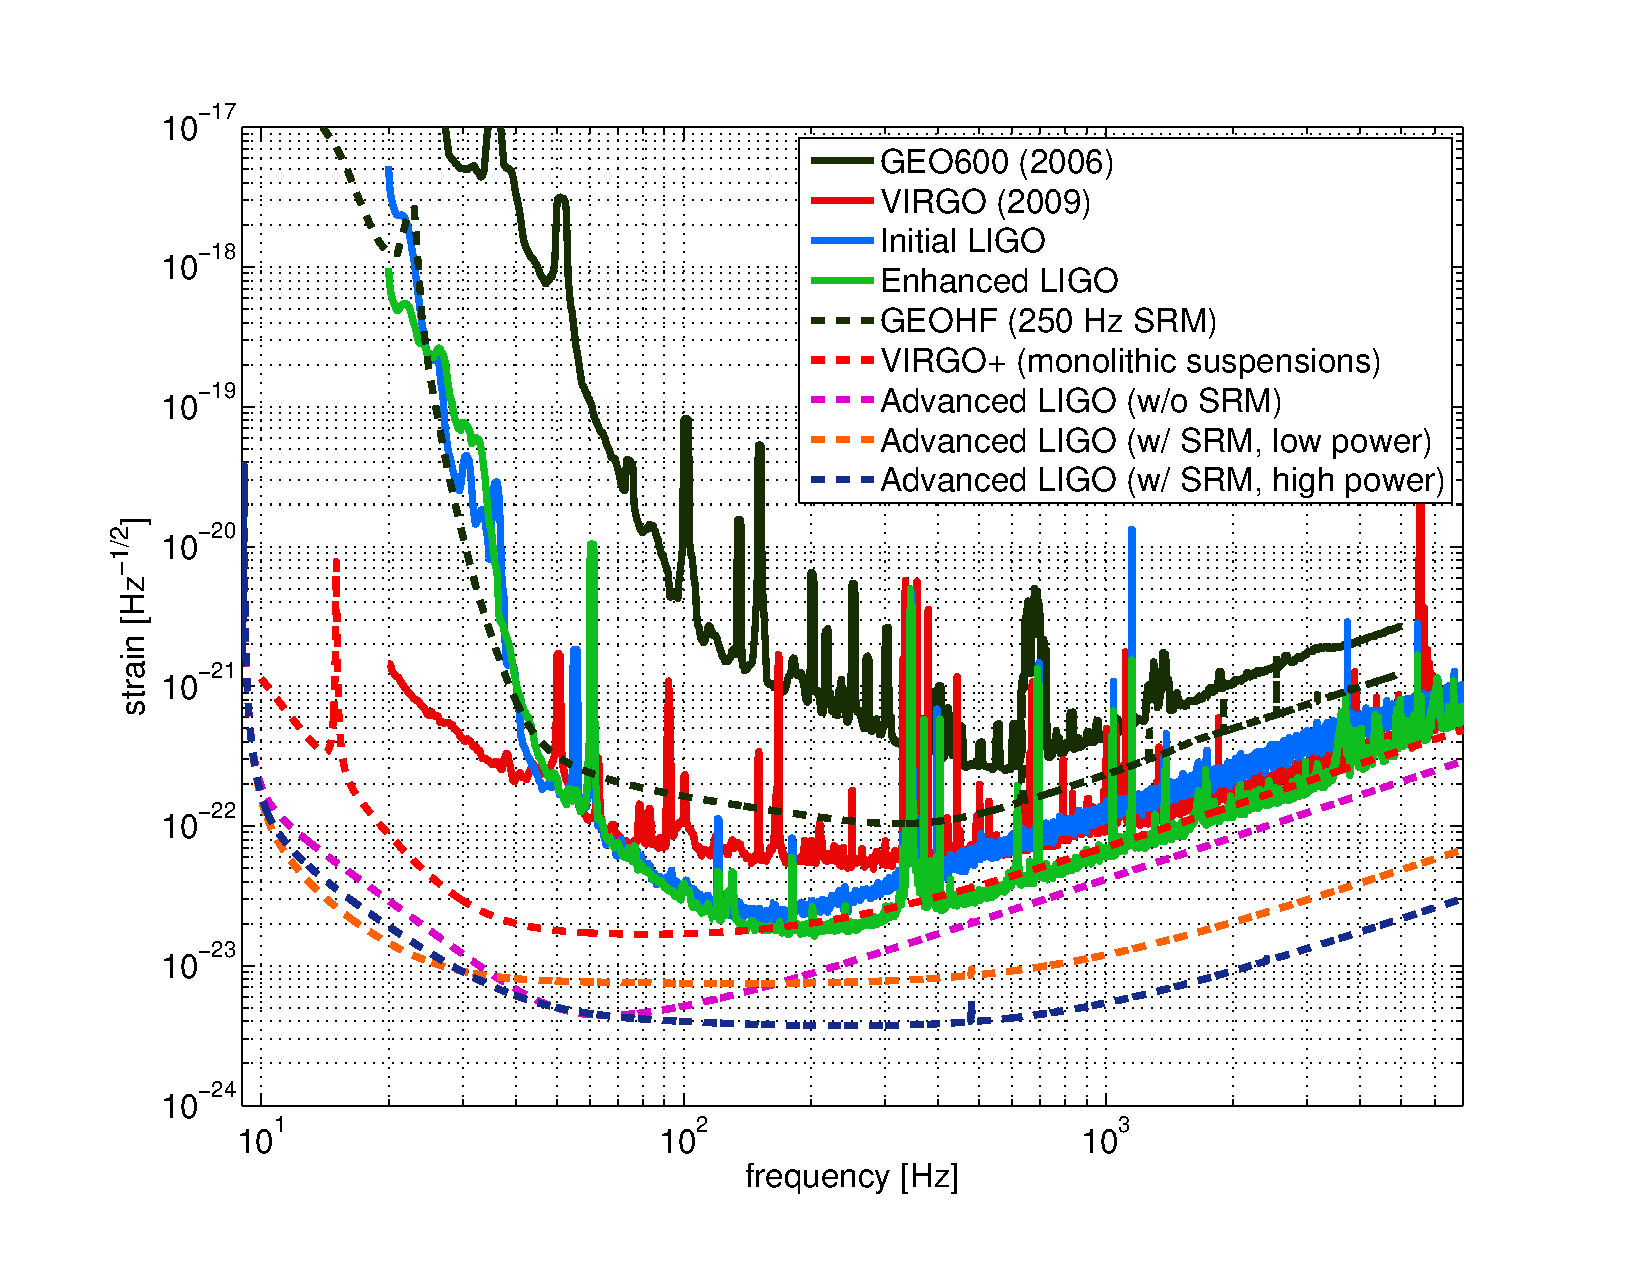
\includegraphics[width=0.7\textwidth]{figures/GWnetwork_sensitivities.pdf}
\caption{Strain sensitivities of LIGO-VIRGO collaboration interferometers.}
\label{fig:h_all}
\end{centering}
\end{figure}

The baseline Advanced LIGO design \cite{AdvLigoSysDesign} improves
upon Initial LIGO by featuring better seismic isolation, the addition
of a signal extraction mirror at the output port, homodyne readout,
and an increase in laser power from 10~W to 200~W. The substantial
increase in laser power improves the shot-noise-limited sensitivity,
but introduces a host of radiation pressure and thermally induced side
effects that must be addressed for proper operation.

The recently completed Enhanced LIGO tested portions of the Advanced
LIGO designs so unforeseen difficulties could be addressed and so that
a more sensitive data taking run could take place. An output mode
cleaner was designed, built and installed, and DC readout of the GW
signal was implemented \cite{Fricke2011DC}. An Advanced LIGO active
seismic isolation table was also built, installed, and tested
\cite{KisselThesis}. In addition, the 10~W Initial LIGO laser was
replaced with a 35~W laser \cite{Frede2007Fundamental}. Accompanying
the increase in laser power, both the Alignment Sensing and Control
and Input Optics were modified. The upgrades of these two subsystems
make up the content of this dissertation. 




\section{Purpose of this work}
The purpose of this work is to demonstrate the capability of an
interferometric gravitational wave detector to operate at several
times the highest of laser powers previously used. To first order,
more power is desirable since strain sensitivity improves by
$\sqrt{P}$ in the high frequency ($>$ several hundred Hz)
shot-noise-limited region. However, as detectors become more sensitive
at low frequencies ($<$ 100 Hz), radiation pressure noise will become
the dominant noise source, making high laser power operation a design
trade-off. Currently, since seismic noise limits low frequency
sensitivity, exploring the technical world of increasing the laser
power is a fruitful adventure.

Operation of Initial LIGO was limited to 7~W input power due to
uncontrolled radiation pressure torque instabilities in the arm
cavities. Explained theoretically by Sidles and Sigg
\cite{Sidles2006Optical}, measured experimentally by Hirose
\cite{Hirose2010Angular}, and modeled by Barsotti
\cite{Barsotti2009modeling}, the effect of radiation pressure torque
on angular alignment needed to be addressed in practice in order for
Enhanced LIGO to succeed in operating at its design power of 30~W. We
present the re-designed Angular Sensing and Control system as
implemented on the Enhanced LIGO detectors and show results of its
performance with up to 20~W input power, demonstrating good agreement
between experiment and model. 

Additional complications of high laser power operation arise from
thermal effects. Absorption of power by optical components induces
thermal lensing which changes the properties of the propagating
laser. The Input Optics, which condition the laser for optimal use in
the interferometer, suffered from thermal absorption of the 7~W of
Initial LIGO. Although not a source of GW strain noise, the thermal
performance of the Input Optics must be good enough so as to not
hinder 




\chapter{Laser Interferometers for Gravitational-wave Detection}

We show in this chapter how a laser interferometer can detect
gravitational wave strain, and we present the basic design principles
of the LIGO detectors. We motivate the desire for higher laser power,
and introduce some of the details of the interferometer that are
relevant for later chapters. To reduce clutter, I do not specify the
polarization of the gravitational wave strain and use simply $h$ for
its symbol.


\section{Measuring Gravitational-wave Strain with Light}
Considering a simple Michelson interferometer consisting of a laser, a
beam splitter, and two end mirrors each a distance $L$ from the beam
splitter, one can understand intuitively why an interferometer can
detect gravitational waves. If an appropriately polarized
gravitational wave is present, it will stretch one arm and compress
the other. For two wave packets leaving the beam splitter at the same
time, each heading down a different arm, the roundtrip travel time for
the light traveling down the stretched arm is longer than that for the
light traveling down the compressed arm. For the stretched arm the
roundtrip travel time is:
\begin{equation}
t_{\mathrm{stretched}} = \frac{2 L}{c} \left( 1 + \frac{h}{2} \right),
\label{eq:trt+} 
\end{equation}
and for the compressed arm the roundtrip travel time is:
\begin{equation}
t_{\mathrm{compressed}} = \frac{2 L}{c} \left( 1 - \frac{h}{2} \right).
\label{eq:trt-} 
\end{equation}
A stationary clock at the beam splitter could, in principle, measure
the non-zero difference in arrival times, $\Delta t = 2Lh/c$, of the
two different wave packets.\footnote{It should be noted that $h$ is
  treated as a constant in Eqs. \ref{eq:trt+} and \ref{eq:trt-}. We
  use the approximation that the gravitational wave wavelength
  $\lambda_{gw}$ is much larger than the Michelson arm length
  $L$. This means that the temporal variation of $h(t)$ is negligible
  during the time it takes the photon to make its roundtrip.}

In practice we send a
continuous electromagnetic wave into the interferometer. The
difference in travel times turns into a difference in phase of
the beams returning to the beamsplitter:
\begin{equation}
\Delta \phi_{\mathrm{MICH}} = \omega \Delta t = \frac{2 L}{c} \omega h,
\label{eq:deltaphi}
\end{equation}
where $\omega$ is the angular frequency of the laser light. We now
introduce the modified Michelson interferometer used in LIGO, and in
this context continue the discussion of strain measurement and
sensitivity.

% reference to treatment as a wave, gauge-independent quantity.



\section{Power-recycled Fabry-P\'{e}rot Michelson Interferometers} 
The LIGO detector configuration is a power-recycled Fabry-P\'{e}rot
Michelson laser interferometer as depicted in
Fig.~\ref{fig:IFOschematic}. A beam splitter (BS) directs 1064~nm
light from a diode-pumped, power amplified, and intensity and
frequency stabilized Nd:YAG laser to the Fabry-P\'{e}rot arms, which are
made of an input test mass mirror (ITM) and an end test mass mirror
(ETM). Both arms are of length $L \approx 4 \text{ km}$ and are set to maintain nearly
perfect destructive interference of the recombined light at the
anti-symmetric (AS) port, where a photodetector is placed to measure
any change in power. A power recycling mirror (RM) at the symmetric
port directs the constructively-interfered light back into the
interferometer.

\begin{figure}
\begin{centering}
\includegraphics{figures/IFOsimple_thesis.pdf}
\caption[Power-recycled Fabry-P\'{e}rot Michelson laser
interferometer]{Power-recycled Fabry-P\'{e}rot Michelson laser
  interferometer.}
\label{fig:IFOschematic}
\end{centering}
\end{figure}

The Fabry-P\'{e}rot arms are a modification to the Michelson that
increases the change in phase measured at the AS port compared to that
for a simple Michelson. Rather than make a single roundtrip down each
arm, the light is trapped by the Fabry-P\'{e}rot cavity, experiencing many
roundtrips before returning to the beam splitter and interfering with
the light from the other arm. The effect is that Eq.~\ref{eq:deltaphi}
for the Fabry-P\'{e}rot Michelson includes a frequency-dependent phase
gain factor, $g_{\phi}(f)$:
\begin{equation}
\Delta \phi = \frac{2 L}{c} \omega g_{\phi}(f) \Delta h.
\label{eq:deltaphi}
\end{equation}
For Enhanced LIGO, $g_{\phi} = 137$ at DC and falls off as $1/f$ after
85~Hz due to the storage time of the light in the arm cavities.


\subsection{DC readout}
\label{sec:DCreadout}
The gravitational wave readout in Enhanced LIGO was not operated
precisely at the dark fringe at the AS port. Instead, it used a small
offset from the quadratic minimum so that small changes in phase linearly
produce power changes as is depicted in Figure~\ref{fig:DCreadout}. The
offset used was $\phi_0 \approx 6 \times 10^{-5}$~rad; the
technique is a form of homodyne detection called DC readout~\cite{Fricke2011DC}.

With a DC offset, the electric field at the AS port is $E_{AS} =
E_{BS}\sin{(\phi_0 + \Delta\phi)}$. Squaring the electric field and
expanding about $\phi_0$, we determine the power incident on the
photodetector, $P_{AS}$:
\begin{align}
P_{AS} &= P_{BS} \sin^2{(\phi_0 + \Delta\phi)} \\
% &\approx P_{BS}\sin^2{(\phi_0)} + 2P_{BS}\sin{(\phi_0)}\cos{(\phi_0)}\Delta\phi
 &\approx P_{BS}\sin^2{(\phi_0)} + 2P_{BS}\phi_0\Delta\phi
\end{align}
The first term on the right hand side of the expanded $P_{AS}$ is the
DC power due to the static offset from the fringe. The second term on
the right hand side describes how a change in phase at the beam
splitter is converted to a change in power:
\begin{equation}
\frac{d P_{AS}}{d \phi_{BS}} =2 P_{BS} \phi_0 
%\mathrm{phase\ optical\ gain} = \frac{4 L}{c} P_{BS} \phi_0 \omega \phi_g(f) h.
\label{eq:dP_dphi}
\end{equation}
This relationship is linear and proportional to the power at the beam
splitter. Throughout this dissertation, when we refer to signals
falling in a \emph{linear regime}, we mean that they are small enough
to be well modeled by a tangent to the actual response, just as for
the case described here regarding small phase signals.

\begin{figure}
\begin{centering}
\includegraphics{figures/DCreadout.pdf}
\caption[The DC readout dark fringe]{The DC readout dark fringe. The
  AS port is not kept at the dark fringe, but is slightly offset by
  $\phi_0$. Changes in phase at the beam splitter are a linear
  function of power.}
\label{fig:DCreadout}
\end{centering}
\end{figure}



\subsection{DARM}
The differential arm length (commonly known as DARM) is of central interest. This
is the length degree of freedom affected by gravitational waves. It is
defined as
\begin{equation}
\mathrm{DARM} := L_- := L_x - L_y
\end{equation}
where $L_x$ and $L_y$ are the lengths of the $x$-arm and $y$-arm,
respectively. When there is no gravitational wave, $L_-=0$, but in the
presence of a gravitational wave, the DARM signal is:
\begin{equation}
L_- = Lh
\label{eq:DARMandh}
\end{equation}
We see that $L$ is the conversion factor between GW strain and DARM.



\subsection{DARM Optical Gain}
The DARM optical gain tells how displacement is converted to power at
the AS port and has units of Watts per meter. Combining
Eqs.~\ref{eq:deltaphi}, \ref{eq:dP_dphi}, and \ref{eq:DARMandh}, the
DARM optical gain of the LIGO interferometer with DC readout is:
\begin{equation}
\frac{d P_{AS}}{dL_-} = \frac{4}{c} P_{BS} \phi_0 \omega g_{\phi}.
\label{eq:opticalgain}
\end{equation}




\section{Signal Versus Noise} 
From Eq.~\ref{eq:opticalgain} we see three fundamental
ways to increase the DARM optical gain and therefore produce more
power at the AS port for a given GW strain:
\begin{enumerate}
\item Make the arms longer. \vspace{-10 pt}
\item Increase the power at the beamsplitter. \vspace{-10 pt}
\item Increase the phase gain of the Fabry-P\'{e}rot arms.
\end{enumerate}
Our ability to detect gravitational wave strain is
dependent not only on the optical gain, but also on the detector noises,
which will mask a weak GW signal. No matter how large a
signal one might have, it won't be found confidently, or at all, if
there is too much noise. 


\subsection{Noises}
The sources of noise which contaminate the detector's output can be 
generally grouped into two categories:
\begin{enumerate}
\item displacement noise \vspace{-10 pt}
\item sensing noise
\end{enumerate}
Displacement noises are those that create real motion of the mirrors
(including the DARM degree of freedom), while sensing noises are those
that arise in the process of measuring the electric field at the 
detector's output.

The primary displacement noise that plagues terrestrial laser
interferometers is motion of the ground, i.e. seismic noise.  Thermal
motion of the mirrors and their suspensions are another source of
displacement noise. 

%% \begin{equation}
%% F(f) = \sqrt{4k_BTb(f)},
%% \end{equation}
%% where $k_B$ is Boltzmann's constant, $T$ is temperature, and $b$ is
%% the mirror's dissipation.

%%  With improvements in seismic isolation, future
%% detectors will be limited at low frequency by photon radiation pressure
%% noise.

The primary sensing noises are electronics (`dark') noise (due to
thermal noise in resistors and electronic amplifiers), and shot
noise, which arises from the Poisson statistics of photon arrival
at the photodetector. Shot noise appears as a
fluctuating power with amplitude spectral density:
\begin{equation}
P_{SN} = \sqrt{2 P h_p \nu}
\label{eq:shotnoise}
\end{equation}
where $P$ is the mean power on the photodiode, $h_p$ is Planck's
constant, and $\nu$ is the frequency of the incident light. Shot noise
is spectrally white.  The detector electronics are typically designed
so that electronics noise is never limiting.

% (with units of W/$\sqrt{\mathrm{Hz}}$) 
\subsection{Noise Floor}
The detector's noise floor is limited by seismic noise below 40~Hz and
by shot noise above 200~Hz.   In general we endeavor to push the noise floor down as far as possible
so that any underlying GW signals will be revealed.  Whether
limited by displacement noise or by sensing noise, the noise floor,
calibrated in strain, can be lowered by increasing the length of the
arms, which acts as the conversion from strain to effective displacement
(Eq.~\ref{eq:DARMandh}).
Further improvements require considering the noise
sources individually.

\subsubsection{Displacement noise floor} 
At frequencies where the noise floor is limited by displacement noise,
simply increasing the DARM optical gain will not help. The mirror
displacements, whether due to gravitational waves or due to ground
motion, are converted into power at the AS port in the exact same
way.   Reduction of displacement noises mainly relies on the development
of more sophisticated seismic isolation systems and mirror suspension
arrangements.

% You should make the point that improvements in the displacement noise
% floor are only linear in the arm length, whereas each additional stage
% of seismic isolation can potentially reduce the displacement noise 
% by 1/f^2.  Make the point that we already have 1/f^n attenuation.  Also, 
% of course, increasing the LIGO arm lengths is not actually an option.

\subsubsection{Sensing noise floor}
The noise floor due to sensing noise is improved by increasing the
optical gain. 
In particular, the contribution due to shot noise  may be found by 
dividing the shot noise amplitude spectral density by the optical gain,
\begin{equation}
h_{shot} = \sqrt{\frac{h_p}{2 P_{BS} \nu}} \frac{c}{4 \pi L g_{\phi}}
\quad \text{W}/\sqrt{\text{Hz}}.
\label{eq:SNL}
\end{equation}

Here we see that the shot noise limit (calibrated in effective strain)
drops with increases in the optical gain. 
Increasing the power in the interferometer improves the shot noise limit
because the optical gain increases more quickly ( $\propto
P_{BS}$, see Eq.~\ref{eq:opticalgain}) than the shot noise amplitude
(which goes like $\sqrt{P_{BS}}$, assuming the DARM offset is held
constant).

Increasing the power at the beam splitter and therefore lowering the
noise floor above 200~Hz is a goal of this work. The power at the BS
is dependent on several quantities:
\begin{itemize}
\item input power \vspace{-10 pt}
\item input efficiency \vspace{-10 pt}
\item power reycling gain
\end{itemize}
Improving the Input Optics allows for greater input power and better
input efficiency. Improving the Angular Sensing and Control allows for
greater input power and better power recycling gain.



% \section{DC readout / more laser power}
% Increasing the laser power in the interferometer is a 

% Shot noise is a Poissonian process: the average number of photons
% striking a detector, $\left<x\right>$, is equal to the variance of the
% mean number of photons, $\left<x^2\right> - \left<x\right>^2$, from a
% given chunk of time $\tau$ to another. For large $\left<x\right>$, the
% distribution becomes Gaussian, but the mean and variance are still
% equivalent. Based on this property and Parseval's theorem, the power
% on a detector due to shot noise is:


%A summary of the noise budget is shown in Fig. \ref{fig:NB}.

% \begin{figure}
% \begin{centering}
% %\includegraphics[width=0.8\textwidth]{figures/.pdf}
% \caption[LIGO noise budget]{Noise budget place holder.}
% \label{fig:NB}
% \end{centering}
% \end{figure}




\section{Controlling the Interferometer}
The ability of the interferometer to operate as described above
requires that the many interferometer
cavities be held on resonance. The motion
of the mirrors in the absence of control is much too large 
--on the order of 1\micron, a full wavelength!--to maintain resonance.
The motion of the interferometer mirrors must therefore be controlled.
A feedback control system is implemented to hold the system sufficiently
near (for DARM, within $\sim 10^{-13}$ m) the intended operating point so that the response to residual
deviations remains linear.  (Calibration of the detector must take
into account the action of the control system.)

% Since the strain sensitivity is determined
% by mathematically undoing the (carefully measured) effect of the
% control system on DARM, control does not directly improve the strain
% sensitivity. The purpose length control does serves is to make the
% strain measurement possible. For other degrees of freedom, such as
% angular motion, only the controlled residual matters ..  Control,
% however, introduces noise so there is a fine balance that must be
% found between too much and too little control.

% Design considerations for the control loops include how much motion at
% what frequencies can be tolerated, and the signal to noise ratio of
% the motion sensor.


% \subsection{RF Sidebands}
% Phase modulation multiplies carrier light with field
% $E_0e^{i\omega t}$ by $e^{i \Gamma \sin{(\Omega t)}}$, where $\Gamma$
% is the modulation index and $\Omega$ is the frequency of the phase
% modulation. Using the Jacobi-Anger expression,
% \begin{equation}
% e^{i z \sin{\theta}} = \sum_{n=-\infty}^{\infty} J_n(z) e^{i n \theta},
% \end{equation}
% where $J_n$ are the Bessel functions, we can write the first few terms
% (n = 0, 1, -1) of the phase-modulated field:
% \begin{equation}
% E_{modulated} = E_0 J_0(\Gamma) e^{i\omega t} + E_0 J_1(\Gamma)
% e^{i(\omega + \Omega) t} + E_0 J_{-1}(\Gamma)
% e^{i(\omega - \Omega) t} + ...
% \end{equation}
% We see that both an upper and lower primary sideband are created, with
% frequencies $\omega + \Omega$ and $\omega - \Omega$. Phase modulation
% does produce an infinite number of sidebands, yet the amplitude of the
% Bessel function decays rapidly with higher $|n|$, so only this first
% set of sidebands are significant.




\subsection{Digital Control in LIGO}
Although the interferometer is an analog instrument, it is interfaced
through a digital control system. The analog sensor signals are sent
through analog-to-digital converters (ADCs), digitally filtered, and
then sent through digital-to-analog converters (DACs) before returning
to the interferometer's actuators as control signals. The 
digital control system allows complex filters to be implemented and
tuned from a comfortable control-room environment.

The various LIGO subsystems operate at different sample rates.  The
length sensing and control (LSC) subsystem, which measures and
controls DARM, in addition to other length degrees of freedom,
operates at 16384 samples/second, while the angular sensing and
control (ASC) sytem, which maintains mirror alignment, operates at
2048 samples/second.  In addition to the all-important DARM channel,
many other auxiliary data streams are permanently recorded.

% There are a select few control systems that remain completely analog, like
% the laser intensity stabilization servo (ISS). When the frequencies of
% interest extend beyond several tens of thousands of Hz, the use of
% computers becomes impractical.




\subsection{Mirror Suspension and Actuation}
\label{sec:suspension}
The primary interferometer optics are suspended in vacuum so that they
act like free masses at the frequencies in the GW detection band, and
so that they are isolated from ground motion. Each mirror is hung from
a single wire that loops around the bottom of the barrel of the mirror
as shown in Fig.~\ref{fig:suspension}. Stand-offs glued just above the
mirror's center of mass on both sides of the barrel mark the final
point of contact of the wire with the mirror, and both ends of the
wire are clamped to the top of a suspension cage.

\begin{figure}
\begin{centering}
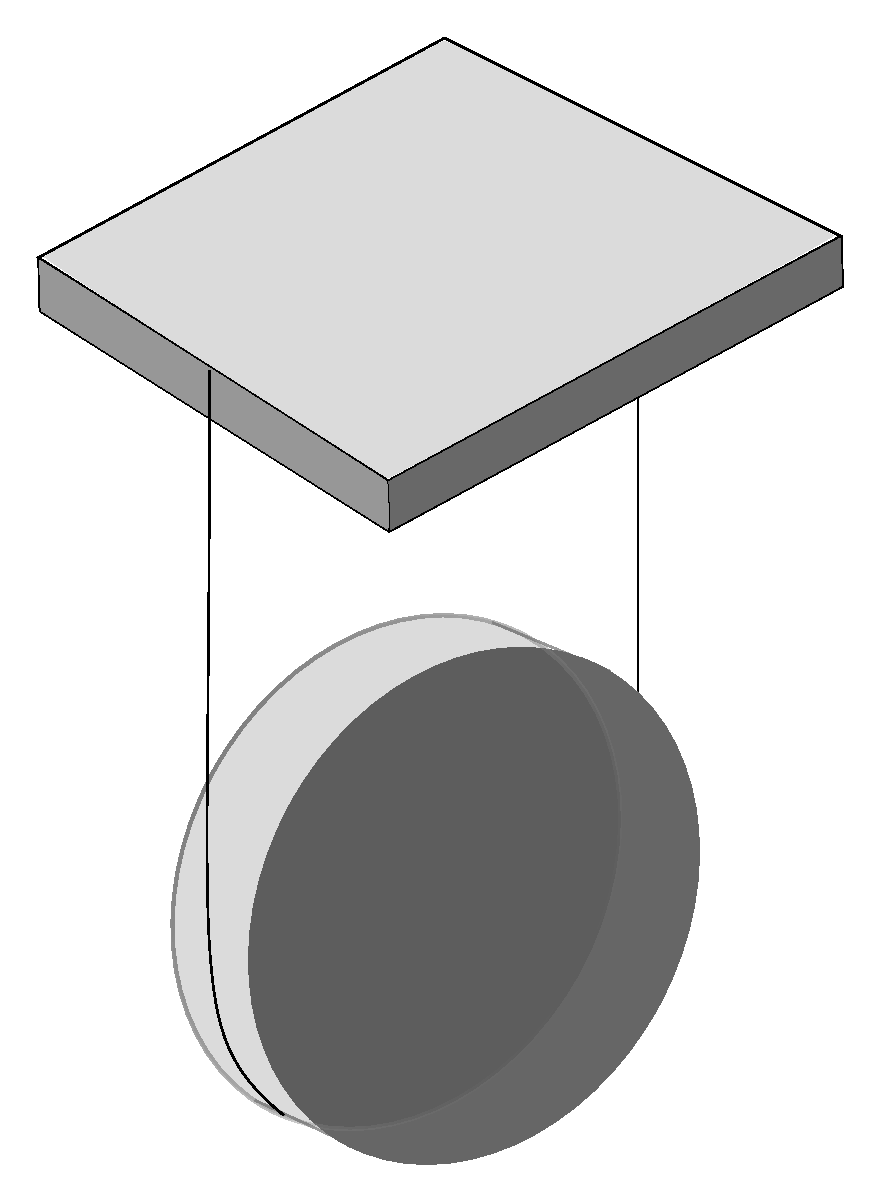
\includegraphics[width=0.3\textwidth]{/Users/kate/kate-thesis/figures/suspension.pdf}
\caption[Sketch of a LIGO suspension]{Sketch of a LIGO suspension.}
\label{fig:suspension}
\end{centering}
\end{figure}

Each mirror is equipped with four optical sensor and electro-magnetic
(OSEM) actuators for rough sensing and fine control of the mirror position and orientation. Magnets arranged
to form the four corners of a square are glued on the mirror's back
surface which are enveloped by the OSEM solenoid coil. 
The currents through each coil may be driven independently.
Length control of the
cavities, for instance, sends current of the same magnitude through
each coil on a given mirror to provide a piston force for changing the
mirror's position.  OSEM sensing is accomplished through simple shadow
sensors.

To avoid thermal noise, the mirror suspensions are designed to minimize 
dissipation.
Damping for the large optics is achieved through
electronic servos.  Motion of the optics corresponding to a change
in cavity length is damped using simple velocity damping servoes
implemented using the OSEM sensors and actuators, while angular
motion is sensed via optical levers.
The optical levers provide velocity damping\footnote{
The open loop transfer function of the optical lever
servo is described in Appendix~\ref{sec:oplevOLG}.
} only (no DC control) between
0.2~Hz and 2~Hz. 

% The suspensions are AC damped at all times for each of the large
% optics through optical lever witnesses. Keeping the mirrors quiet
% enough with respect to their local ground is necessary to allow for
% the initial locking of the interferometer, so each suspended optic,
% small and large, is quieted by its OSEM signals during the initial
% locking stages. After the interferometer is locked, the angular OSEM
% feedback is turned off, and the position OSEM feedback remains.

\section{Summary}
The modified Michelson interferometer provides a robust foundation on
which to build a gravitational wave detector in which fluctuating
gravitational wave strains are transduced into measurable optical
power fluctuations.  For the interferometer to operate properly, the
mirrors positions and orientations must be controlled.  The noise
floor of the interferometer may be improved in the shot noise
dominated regime by increasing the laser power circulating in the
interferometer.  Increases in laser power, however, create several
challenges; two such challenges are addressed in this thesis: coping
with the higher power in the interferometer's input optics (Chapter 3)
and dealing with radiation pressure induced angular instabilities
caused by high power in the interferometer's arm cavities (remaining
chapters).

%\chapter{INPUT OPTICS DESIGN AND CHARACTERIZATION}

\section{Function of the Input Optics}
\label{sec:role}

\begin{figure}
\begin{centering}
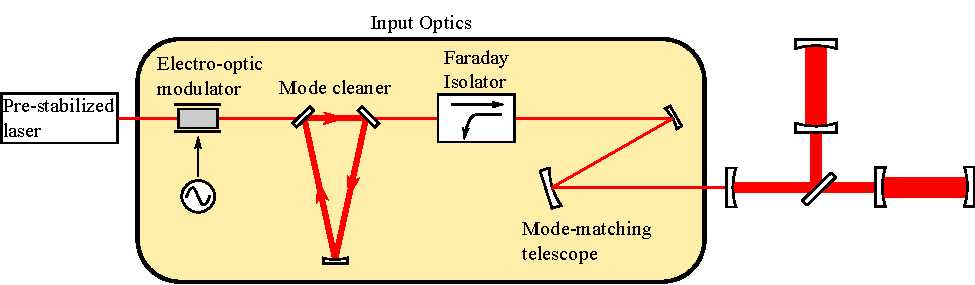
\includegraphics{figures/InputOpticsBlock_thesis.pdf}
\caption[Block diagram of the Input Optics subsystem.]{Block diagram
  of the Input Optics subsystem. The IO is located between the
  pre-stabilized laser and the recycling mirror and consists of four
  components: electro-optic modulator, mode cleaner, Faraday isolator,
  and mode-matching telescope. The electro-optic modulator is the only
  IO component outside of the vacuum system. Diagram is not to scale.}
\label{fig:IOblock}
\end{centering}
\end{figure}

The Input Optics (IO)\footnote{The Input Optics was originally called
  the Input-Output Optics (IOO).} is one of the primary subsystems of the LIGO
interferometers. Its purpose is to deliver an aligned, spatially
pure, mode-matched beam with phase-modulation sidebands to the
power-recycled Fabry-Perot Michelson interferometer. The IO also

prevents reflected or backscattered light from reaching the laser and
distributes the control sidebands reflected from the interferometer
(designated the \emph{reflected port}) to photodiodes for sensing and
controlling the length and alignment of the interferometer. In
addition, the IO provides an intermediate level of frequency
stabilization and must have high overall optical efficiency. It must
perform these functions without limiting the strain sensitivity of the
LIGO interferometer.  Finally, it must operate robustly and
continuously over years of operation. The conceptual design is found
in Ref.~\citep{Camp1996InputOutput}.

As shown in Figure~\ref{fig:IOblock}, the Input Optics subsystem
consists of four principle components located between the
pre-stabilized laser and the power recycling mirror:
\begin{itemize}
\item electro-optic modulator (EOM) \vspace{-10 pt}
\item mode cleaner cavity (MC) \vspace{-10 pt}
\item Faraday isolator (FI) \vspace{-10 pt}
\item mode-matching telescope (MMT)
\end{itemize}
Each element is a common building block of many optical experiments
and not unique to LIGO. However, their roles specific to the
successful operation of interferometry for gravitational-wave
detection are of interest and demand further attention. Here, we
briefly review the purpose of each of the IO components;
further details about the design requirements are in
Ref.~\citep{Camp1997Input}.




\subsection{Electro-optic Modulator} 
The Length Sensing and Control (LSC) and Angular Sensing and Control
(ASC) subsystems require phase modulation of the laser light at RF
frequencies. This modulation is produced by an EOM, generating
sidebands of the laser light which act as references against which
interferometer length and angle changes are measured
\citep{Fritschel2001Readout}. The sideband light must be either
resonant only in the recycling cavity or not resonant in the
interferometer at all. The sidebands must be offset from the carrier
by integer multiples of the MC free spectral range so that
neither MC length fluctuations nor phase modulation of the sidebands
(due to phase noise of the RF oscillator) are converted to amplitude modulation.


\subsection{Mode Cleaner}
Stably aligned cavities, limited non-mode-matched (junk) light, and a
frequency and amplitude stabilized laser are key features of any ultra
sensitive laser interferometer. The mode cleaner, at the heart of the
IO, plays a major role to this effect.

A three-mirror triangular ring cavity, the mode cleaner suppresses
laser output not in the fundamental TEM$_{00}$ mode, serving two major
purposes. It enables the robustness of the ASC since higher order
modes would otherwise contaminate the angular sensing signals of the
interferometer. Also, all non-TEM$_{00}$ light on the length sensing
photodiodes, including those used for the GW readout, contributes shot
noise but not signal and therefore diminishes the signal to noise
ratio. The mode cleaner is thus largely responsible for achieving an
aligned, minimally shot-noise-limited interferometer.

The MC also plays an active role in laser frequency
stabilization \citep{Fritschel2001Readout}, which is necessary for
ensuring that the signal at the anti-symmetric port is due to arm
length fluctuations rather than laser frequency fluctuations. In
addition, the MC passively suppresses beam jitter at frequencies above
10~Hz.

% The mode cleaner also plays an active role in laser frequency
% stabilization \citep{Fritschel2001Readout}. A frequency-stabilized laser is
% necessary for ensuring that the signal at the anti-symmetric port is
% due to arm length fluctuations rather than laser frequency
% fluctuations. In principle, the near-equal two-arm geometry of LIGO facilitates
% this distinction, but imbalances between the arms allow frequency
% noise to couple into the gravitational wave channel. At low
% frequencies ($<$~100 Hz) the average interferometer arm length drives
% the mode cleaner length, which in turn adjusts the laser frequency. At
% high frequencies (up to 20~kHz), the common arm length adds an
% electronic offset to the MC error point, also resulting in a shift of
% the laser frequency. As a result, the light transmitted through the MC
% is matched to the very quiet arms.
 
% The mode cleaner acts as a passive laser amplitude fluctuation
% filter. Laser power fluctuations that couple to the antisymmetric port
% cause noise in the GW readout.  The mode cleaner suppresses laser
% amplitude noise above its pole frequency of about 4500~Hz. In
% addition, the MC passively suppresses beam jitter at frequencies above
% 10~Hz.


\subsection{Faraday Isolator}
Faraday isolators are four-port optical devices which utilize the
Faraday effect to allow for non-reciprocal polarization switching of
laser beams.  Any backscatter or reflected light from the interferometer (due to
impedance mismatch, mode mismatch, non-resonant sidebands, or signal)
needs to be diverted to protect the laser from back propagating light,
which can introduce amplitude and phase noise.  This diversion of the
reflected light is also necessary for extracting length and angular
information about the interferometer's cavities. The Faraday isolator
fulfils both needs.


\subsection{Mode-matching Telescope}
The lowest-order mode cleaner and arm cavity spatial eigenmodes need
to be matched for maximal power buildup in the interferometer. The
mode-matching telescope is a set of three suspended concave mirrors
between the mode cleaner and interferometer that expand the beam from
a radius of 1.6~mm at the mode cleaner waist to a radius of 37~mm at
the recycling mirror as shown in Figure~\ref{fig:ioprofile}. The MMT
should play a passive role by delivering properly shaped light to the
interferometer without introducing beam jitter or any significant
aberration that can reduce mode coupling.

\begin{figure}
\begin{centering}
\includegraphics{figures/ioprofile1W.pdf}
\caption[Beam profile through the Input Optics]{Beam profile through
  the Input Optics. The starting point is the mode cleaner waist and
  the changes in trajectory are due to the mode-matching telescope
  mirrors.}
\label{fig:ioprofile}
\end{centering}
\end{figure}
% /Users/kate/work/2010/09/23/1W/forplotting

\section{Thermal Problems in Initial LIGO}
\label{sec:problems}
The Initial LIGO interferometers were equipped with a 10~W laser, yet
operated with only 7~W input power due to power-related problems with
other subsystems. The EOM was located in the 10~W beam and the other
components experienced anywhere up to 7~W power. The 7~W operational
limit was not due to the failure of the Input Optics; however, many
aspects of the IO performance did degrade with power.

One of the primary problems of the Initial LIGO Input Optics
\citep{Adhikari1998Input} was thermal deflection of the back
propagating beam due to thermally-induced refractive index gradients
in the Faraday isolator. A significant beam drift between the
interferometer's locked and unlocked states led to clipping of the
reflected beam on the photodiodes used for length and alignment
control. Our measurements determined a deflection of approximately
100~\microrad/W in the FI.  This was mitigated at the time by the
design and implementation of an active beam steering servo on the beam
coming from the isolator.

There were also known limits to the power the IO could sustain.
Thermal lensing in the Faraday isolator optics began to alter
significantly the beam mode at powers greater than 10~W, leading to a
several percent reduction in mode matching to the interferometer
\citep{UFLIGOGroup2006Upgrading}.  Additionally, the absorptive FI
elements would create thermal birefringence, degrading the optical
efficiency and isolation ratio with power
\citep{Khazanov1999Investigation}.  The Initial LIGO New Focus
electro-optic modulators had an operational power limit of around
10~W. There was a high risk of damage to the crystals under the stress
of the 0.4~mm radius beam. Also, anisotropic thermal lensing with
focal lengths as severe as 3.3~m at 10~W made the EOMs unsuitable for
much higher power. Finally, the mode cleaner mirrors exhibited high
absorption (as much as 24 ppm per mirror), enough that thermal lensing
of the MC optics at Enhanced LIGO powers would induce higher order
modal frequency degeneracy and result in a power-dependent mode
mismatch into the interferometer \citep{Bullington2008Modal,
  Arain2007Note}. In fact, as input power increased from 1~W to 7~W
the mode matching decreased from 90\% to 83\%.

In addition to the thermal limitations of the Initial LIGO IO, optical
efficiency in delivering light from the laser into the interferometer
was not optimal. Of the light entering the Input Optics chain, only
60\% remained by the time it reached the power recycling
mirror. Moreover, because only 90\% at best of the light at the
recycling mirror was coupled into the arm cavity mode, room was left
for improvement in the implementation of the MMT.



\section{Enhanced LIGO Input Optics Design}
\label{sec:design}
The Enhanced LIGO IO design addressed the thermal effects that
compromised the performance of the Initial LIGO IO, and accommodated
up to four times the power of Initial LIGO. Also, the design was a
prototype for handling the 165~W laser planned for Advanced
LIGO. Because the adverse thermal properties of the Initial LIGO IO
(beam drift, birefringence, and lensing) are all attributable
primarily to absorption of laser light by the optical elements, the
primary design consideration was finding optics with lower absorption
\citep{UFLIGOGroup2006Upgrading}. Both the EOM and the FI were
replaced for Enhanced LIGO. Only minor changes were made to the MC and
MMT. A detailed layout of the Enhanced LIGO IO is shown in Figure
\ref{fig:IOschematic} and photographs are in
Figure~\ref{fig:IOpictures}.

\begin{sidewaysfigure}
\begin{centering}
\includegraphics[width=1.0\textwidth]{figures/iopaperIO_withHam2.pdf}
\caption[Enhanced LIGO Input Optics optical and sensing
  configuration]{Enhanced LIGO Input Optics optical and sensing
  configuration. The HAM1 (horizontal access module) vacuum chamber is
  featured in the center, with locations of all major optics
  superimposed. HAM2 is shown on the right, with its components. These
  tables are separated by 12~m. The primary beam path, beginning at
  the pre-stabilized laser and going to the power recycling mirror, is
  shown in red as a solid line, and auxiliary beams are different
  colors and dotted. The MMTs, MCs, and steering mirror (SM) are
  suspended; all other optics are fixed to the seismically isolated
  table. The laser and sensing and diagnostic photodiodes are on
  in-air tables.}
\label{fig:IOschematic}
\end{centering}
\end{sidewaysfigure}

\begin{figure}
\begin{centering}
\subfigure{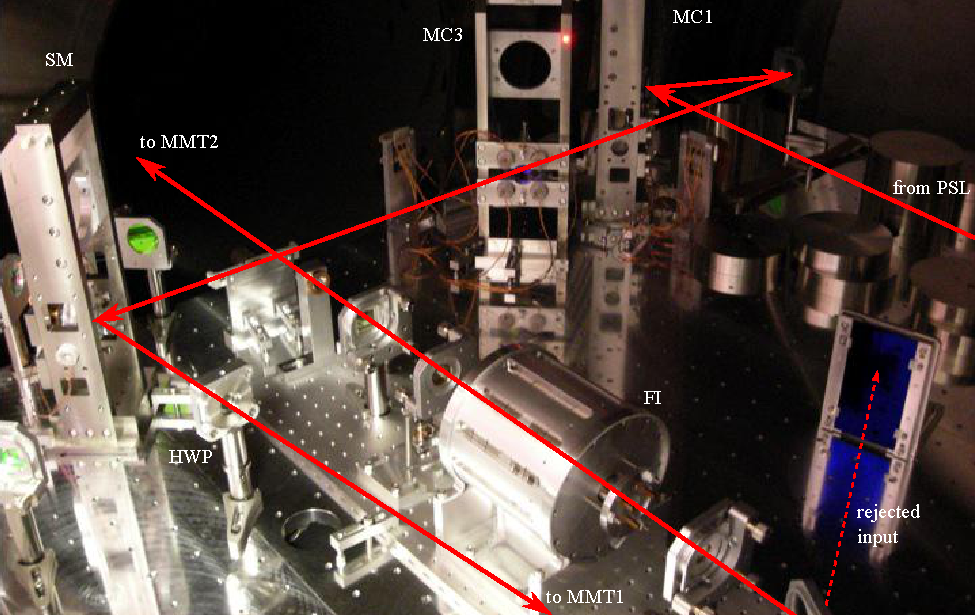
\includegraphics[width=1.0\textwidth]{figures/HAM1_view1.pdf}}
\subfigure{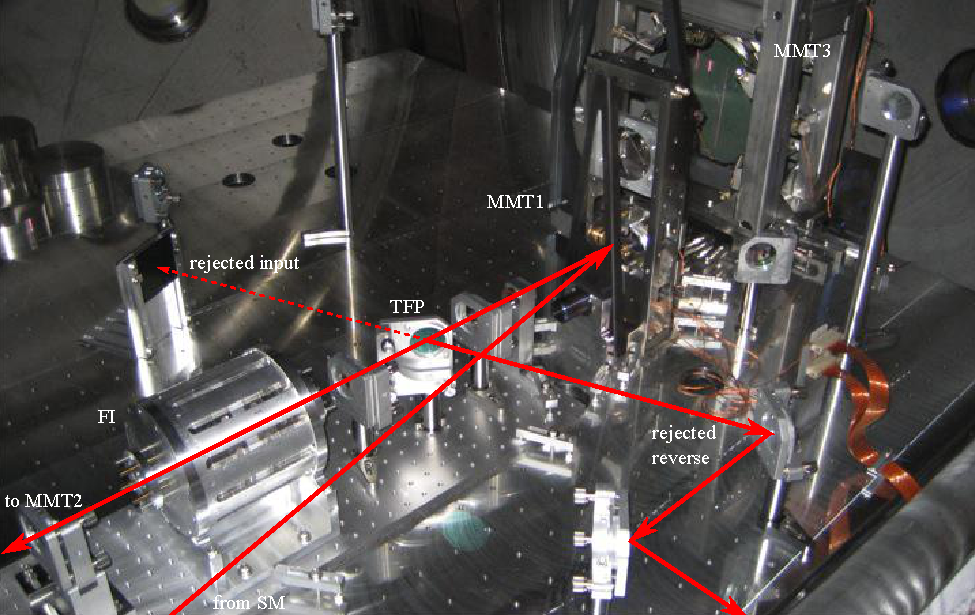
\includegraphics[width=1.0\textwidth]{figures/HAM1_view2.pdf}}
\caption[Photographs of the Enhanced LIGO HAM1 Input Optics \emph{in
  situ}]{Photographs of the Enhanced LIGO HAM1 Input Optics \emph{in
    situ} with a drawing of the beam path superimposed. Photographs
  courtesy of Katherine Dooley.}
\label{fig:IOpictures}
\end{centering}
\end{figure}


\subsection{Electro-optic Modulator Design}
We replaced the commercially-made New Focus 4003 resonant phase
modulator of Initial LIGO with an in-house EOM design and
construction. Both a new crystal choice and architectural design
change allow for superior performance.

The Enhanced LIGO EOM design uses a crystal of rubidium titanyl
phosphate (RTP), which has at most 1/10 the absorption coefficient at
1064 nm of the lithium niobate (LiNbO$_3$) crystal from Initial
LIGO. At 200~W the RTP should produce a thermal lens of 200 m and
higher order mode content of less than 1\%, compared to the 3.3~m lens
the LiNbO$_3$ produces at 10~W. The RTP has a minimal risk of damage,
since it has both twice the damage threshold of LiNbO$_3$ and is
subjected to a beam twice the size of that in Initial LIGO. RTP and
LiNbO$_3$ have similar electro-optic coefficients. Also, RTP's $dn/dT$
anisotropy is 50\% smaller. Table \ref{tab:EOMcrystals} compares the
properties of most interest of the two crystals.

\begin{table}
\centering
\caption[Comparison of selected properties of the Initial and Enhanced
LIGO EOM crystals]{Comparison of selected properties of the Initial and Enhanced
  LIGO EOM crystals, LiNbO$_3$ and RTP, respectively. RTP was
  preferred for Enhanced LIGO because of its lower absorption,
  superior thermal properties, and similar 
  electro-optic properties \citep{UFLIGOGroup2006Upgrading}.}  
\begin{tabular}{l l r@{}l r@{}l}
\hline
 & units & \multicolumn{2}{l}{LiNbO$_3$} & \multicolumn{2}{l}{RTP} \\
\hline
damage threshold & MW/cm$^2$ & 280 & & $>$600 & \\
absorption coeff. at 1064 nm & ppm/cm & $<$5000 & & $<$500 & \\
electro-optic coeff. ($n_z^3 r_{33}$) & pm/V & 306 & & 239 & \\
$dn_y/dT$ & 10$^{-6}$/K & 5 & .4 & 2 & .79 \\
$dn_z/dT$ & 10$^{-6}$/K & 37 & .9 & 9 & .24 \\
\hline
\end{tabular}
\label{tab:EOMcrystals}
\end{table}

We procured the RTP crystals from Raicol and packaged them into
specially-designed, custom-built modulators. The crystal dimensions are
$4 \times 4 \times 40$ mm and their faces are wedged by $2.85^\circ$
and anti-reflection (AR) coated. The wedge serves to separate the
polarizations and prevents an etalon effect, resulting in a
suppression of amplitude modulation. Only one crystal is used in the
EOM in order to reduce the number of surface reflections. Three
separate pairs of electrodes, each with its own resonant LC circuit,
are placed across the crystal in series, producing the three required
sets of RF sidebands: 24.5~MHz, 33.3~MHZ and 61.2~MHz. A diagram is
shown in Figure \ref{fig:EOM}. Reference
\citep{Quetschke2008ElectroOptic} contains further details about the
modulator architecture.

\begin{figure}
\begin{centering}
  \subfigure[]{\includegraphics{figures/EOMthesis.pdf}}
  \subfigure[]{\includegraphics{figures/EOMcircuit_thesis.pdf}}
  \caption[Electro-optic modulator design]{Electro-optic modulator
    design. A) The single RTP crystal is sandwiched between three sets
    of electrodes that apply three different modulation
    frequencies. The wedged ends of the crystal separate the
    polarizations of the light. The p-polarized light is used in the
    interferometer. B) A schematic for each of the three impedance
    matching circuits of the EOM. For the three sets of electrodes,
    each of which creates its own $C_{crystal}$, a capacitor is placed
    parallel to the LC circuit formed by the crystal and a hand-wound
    inductor.  The circuits provide 50~$\Omega$ input impedance on
    resonance and are housed in a separate box from the crystal.}
\label{fig:EOM}
\end{centering}
\end{figure}

\subsection{Mode Cleaner Design}
The mode cleaner is a suspended 12.2~m long triangular ring cavity
with finesse $\mathcal{F}$=1280 (refer to Appendix~\ref{sec:MCpole}
for a measurement of the finesse) and free spectral range of
12.243~MHz. The three mirror architecture was selected over the
standard two mirror linear filter cavity because it acts as a
polarization filter and because it eliminates direct path back
propagation to the laser \citep{Raab1992Estimation}.  A pick-off of the
reflected beam is naturally facilitated for use in generating control
signals. A potential downside to the three mirror design is the
introduction of astigmatism, but this effect is negligible due to the
small opening angle of the MC. 

The MC has a round-trip length of 24.5~m. The beam waist has a radius of
1.63~mm and is located between the two 45$^\circ$ flat mirrors, MC1 and
MC3. See Figure \ref{fig:IOschematic}). A concave third mirror, MC2,
18.15~m in radius of curvature, forms the far point of the mode
cleaner's isosceles triangle shape. The power stored in the MC is 408
times the amount coupled in, equivalent to about 2.7~kW in Initial
LIGO and at most 11~kW for Enhanced LIGO. The peak irradiances are
32~kW/cm$^2$ and 132~kW/cm$^2$ for Initial LIGO and Enhanced LIGO,
respectively.

The mode cleaner mirrors are 75 mm in diameter and 25 mm thick. The
substrate material is fused silica and the mirror coating is made of
alternating layers of silica and tantala. In order to reduce the
absorption of heat in these materials and therefore improve the
transmission and modal quality of the beam in the mode cleaner, we
removed particulate by drag wiping the surface of the MC mirrors with
methanol and optical tissues. The mode cleaner was otherwise identical
to that in Initial LIGO.



\subsection{Faraday Isolator Design}
The Enhanced LIGO Faraday isolator design required not only the use of
low absorption optics, but additional design choices to mitigate any
residual thermal lensing and birefringence. In addition, trade-offs
between optical efficiency in the forward direction, optical isolation
in the backwards direction, and feasibility of physical access of the
return beam for signal use were considered. The result is that the
Enhanced LIGO Faraday isolator needed a completely new architecture
and new optics compared to both the Initial LIGO FI and commercially
available isolators.

Figure \ref{fig:FI} shows a schematic of the Enhanced LIGO Faraday
Isolator. It begins and ends with low absorption calcite wedge
polarizers (CWP). Between the CWPs is a thin film polarizer (TFP), a
deuterated potassium dihydrogen phosphate (DKDP) element, a half-wave
plate (HWP), and a Faraday rotator. The rotator is made of two low
absorption terbium gallium garnet (TGG) crystals sandwiching a quartz
rotator (QR) inside a 7-disc magnet with a maximum field strength of
1.16~T. The forward propagating beam upon passing through the TGG, QR,
TGG, and HWP elements is rotated by $+22.5^\circ - 67.5^\circ +
22.5^\circ + 22.5^\circ = 0^\circ$. In the reverse direction, the
rotation through HWP, TGG, QR, TGG is $-22.5^\circ + 22.5^\circ +
67.5^\circ + 22.5^\circ = 90^\circ$. The TGG crystals are
non-reciprocal devices while the QR and HWP are reciprocal.

\begin{figure}
\begin{centering}
\subfigure{\includegraphics[width=0.9\columnwidth]{figures/FI_cropped2.jpg}}
\subfigure{\includegraphics{figures/FI_thesis.pdf}}
\caption[Faraday isolator photograph and schematic.]{Faraday isolator
  photograph and schematic. The Faraday isolator preserves the
  polarization of the light in the forward-going direction and rotates
  it by 90 degrees in the reverse direction. Light from the MC enters
  from the left and exits at the right towards the interferometer. It
  is ideally p-polarized, but any s-polarization contamination is
  promptly diverted $\sim 10$ mrad by the CWP and then reflected by
  the TFP and dumped. The p-polarized reflected beam from the
  interferometer enters from the right and is rotated to s-polarized
  light which is picked-off by the TFP and sent to the Interferometer
  Sensing and Control (ISC) table. Any imperfections in the Faraday
  rotation of the interferometer return beam results in p-polarized
  light traveling backwards along the original input path. Photograph
  courtesy of Katherine Dooley.}
\label{fig:FI}
\end{centering}
\end{figure}

\subsubsection{Thermal birefringence} 
Thermal birefringence is addressed in the Faraday rotator by the use
of the two TGG crystals and one quartz rotator rather than the typical
single TGG \citep{Khazanov2000Suppression}.  In this configuration,
any thermal polarization distortions that the beam experiences while
passing through the first TGG rotator will be mostly undone upon
passing through the second. The multiple elements in the magnet
required a larger magnetic field than in Initial LIGO.
%\textcolor{blue}{(Add sentence of further explanation.)} 
The 7-disc magnet is 130~mm in diameter and 132~mm long and placed in
housing 155~mm in diameter and 161~mm long. The TGG diameter is 20~mm.

\subsubsection{Thermal lensing}  
Thermal lensing in the Faraday isolator is addressed by including
DKDP, a negative $dn/dT$ material, in the beam path. Absorption of
light in the DKDP results in a de-focusing of the beam, which
partially compensates for the thermal focusing induced by absorption
in the TGGs \citep{Mueller2002Method, Khazanov2004Compensation}.  The
optical path length (thickness) of the DKDP is chosen to slightly
over-compensate the positive thermal lens induced in the TGG crystals,
anticipating other positive thermal lenses in the system.

\subsubsection{Polarizers}  
The polarizers used (two CWPs and one TFP) each offer advantages and
disadvantages related to optical efficiency in the forward-propagating
direction, optical isolation in the reflected direction, and thermal
beam drift. The CWPs have very high extinction ratios ($>10^5$) and
high transmission ($>$ 99\%) contributing to good optical efficiency
and isolation performance. However, the angle separating the exiting
orthogonal polarizations of light is very small, on the order of 10
mrad. This small angle requires the light to travel relatively large distances
before we can pick off the beams
needed for interferometer sensing and control. In addition, thermally
induced index of refraction gradients due to the 4.95$^{\circ}$ wedge
angle of the CWPs result in thermal drift. However, the CWPs for the
Enhanced LIGO Faraday have a measured low absorption of 0.0013
cm$^{-1}$
%(from eLIGO wiki) 
with an expected thermal lens of 60~m at 30~W and drift of less than
1.3 $\mu$rad/W \citep{UFLIGOGroup2006Upgrading}.

The advantages of the thin film polarizer over the calcite wedge
polarizer are that it exhibits negligible thermal drift when compared
with CWPs and it operates at the Brewster angle of 55$^\circ$, thus
diverting the return beam in an easily accessible way. However, the
TFP has a lower transmission than the CWP, about 96\%, and an
extinction ratio of only 10$^3$.

Thus, the combination of CWPs and a TFP combines the best of each to
provide a high extinction ratio (from the CWPs) and ease of reflected
beam extraction (from the TFP). The downsides that remain when using
both polarizers are that there is still some thermal drift from the
CWPs. Also the transmission is reduced due to the TFP and to the fact
that there are 16 surfaces from which light can scatter.

\subsubsection{Heat conduction}
\label{sec:heatconduction}
Faraday isolators operating in a vacuum environment suffer from
increased heating with respect to those operating in air. Convective
cooling at the faces of the optical components is no longer an
effective heat removal channel, so proper heat sinking is essential to
minimize thermal lensing and depolarization. It has been shown that
Faraday isolators carefully aligned in air can experience a dramatic
reduction in isolation ratio ($>$ 10-15 dB) when placed in vacuum
\citep{TheVIRGOCollaboration2008Invacuum}. The dominant cause is the
coupling of the photoelastic effect to the temperature gradient
induced by laser beam absorption. Also of importance is the
temperature dependence of the Verdet constant--different spatial parts
of the beam experience different linear polarization rotations in the presence
of a temperature gradient \cite{Barnes1992Variation}.

\begin{figure}
\begin{centering}
\includegraphics{figures/TGG_scaled.jpg}
\caption[Photograph of an indium-wrapped TGG crystal]{Photograph of TGG crystal
  with indium foil wrapping. Photograph courtesy of Katherine Dooley.}
\label{fig:TGG}
\end{centering}
\end{figure}

To improve heat conduction away from the Faraday rotator optical
components, we designed housing for the TGG and quartz crystals that
provided improved heat sinking to the Faraday rotator. We also wrapped
the TGGs with indium foil as pictured in Figure \ref{fig:TGG} to improve
contact with the housing, and we cushioned the DKDP and the HWP with
indium wire in their aluminum holders. This has the additional effect
of avoiding the development of thermal stresses in the crystals, an
especially important consideration for the very fragile DKDP.


\subsection{Mode-matching Telescope Design}
% from May 31, 2007 elog
The mode matching into the interferometer (at Livingston) was measured
to be at best 90\% in Initial LIGO. Because of the stringent
requirements placed on the LIGO vacuum system to reduce phase noise
through scattering by residual gas, standard opto-mechanical
translators are not permitted in the vacuum; it is therefore not
possible to physically move the mode matching telescope mirrors while
operating the interferometer. Through a combination of needing to move
the MMTs in order to fit the new Faraday isolator on the in-vacuum
optics table and additional measurements and models to determine how
to improve the coupling, a new set of MMT positions was chosen for
Enhanced LIGO. Fundamental design considerations are discussed in
Ref. \citep{Delker1997Design}.



\section{Performance of the Enhanced LIGO Input Optics}
\label{sec:performance}
The most convincing figure of merit for the Input Optics performance
is that the Enhanced LIGO interferometers achieved low-noise operation
with 20 W input power without thermal issues from the
IO. Additionally, the Input Optics were operated successfully up to
the available 30 W of power.  (Instabilities with other interferometer
subsystems limited the Enhanced LIGO science run operation to 20~W.)
We present in this section detailed measurements of the Input Optics
performance during Enhanced LIGO. Specific measurements and results
presented in figures and the text come from Livingston; performance at
Hanford was similar and is included in tables summarizing the results.



\subsection{Optical Efficiency}
The optical efficiency of the Enhanced LIGO Input Optics from EOM to
recycling mirror was 75\%, a marked improvement over the approximate
60\% that was measured for Initial LIGO. A substantial part of the
improvement came from the discovery and subsequent correction of a
6.5\% loss at the second of the in-vacuum steering mirrors directing
light into the MC (refer to Figure \ref{fig:IOschematic}). A 45$^\circ$
reflecting mirror had been used for a beam with an 8$^\circ$ angle of
incidence. Losses attributable to the mode cleaner and Faraday
isolator are described in the following sections. A summary of the IO
power budget is found in Table \ref{tab:pwrbudget}.

\begin{table}
\centering
\caption[Enhanced LIGO Input Optics power budget.]{Enhanced LIGO Input
  Optics power budget. Errors are $\pm 1\%$, except for the TFP loss
  whose error is $\pm 0.1\%$. The 
  composite mode cleaner transmission is the percentage of power after the MC to
  before the MC and is the product of the MC visibility and
  transmission. Initial LIGO values,
  where known, are included in parentheses and have errors of several percent.}
\begin{tabular}{l r@{}l r@{}l}
\hline
 & \multicolumn{2}{l}{Livingston} & \multicolumn{2}{l}{Hanford} \\
\hline
Mode cleaner visibility & 92 & \% & 97 & \% \\
Mode cleaner transmission & 88 & \% & 90 & \% \\
Composite MC transmission & 81 & \% (72\%) & 87 & \% \\
Faraday transmission &       93 & \% (86\%) & 94 & \% (86\%) \\
\hspace{0.5cm} - Thin film polarizer loss & 4 & .0\% & 2 & .7\% \\ 
IO efficiency (PSL to RM) & 75 & \% (60\%) & 82 & \% \\
\hline
\end{tabular}
\label{tab:pwrbudget}
\end{table}


\subsubsection{Mode cleaner losses} 
The mode cleaner was the greatest single source of power loss in both
Initial and Enhanced LIGO. The mode cleaner visibility, defined here as
\begin{equation}
\mbox{visibility} = \frac{P_{\mathrm{in}} - P_{\mathrm{reflected}}}{P_{\mathrm{in}}},
\end{equation}
the ratio of the amount of light coupled into the MC to the amount
impinging the MC input mirror, was 92\%. Visibility
reduction is the result of higher order mode content of $P_{\mathrm{in}}$
and mode mismatch into the MC. The visibility was constant within
0.04\% up to 30~W input power at both sites, providing a positive
indication that thermal aberrations in the MC and upstream
were negligible.

Of the light coupled into the MC, 88\% was transmitted,
corresponding to an average loss of 98 ppm per mirror.  The scatter
loss, $[4 \pi \sigma_{rms} / \lambda]^2$, is expected to be 22
ppm/mirror based on the mirrors' measured root mean square surface
microroughness of $\sigma_{rms}< 0.4$ nm \cite{1998Component}. Part of
the discrepancy between expectation and measurement was determined to
come from poor or damaged AR coatings. We measured a 1.3\% reflection
from the AR coatings on MC mirrors at both Livingston and Hanford, a
transmitted power loss equivalent to 10~ppm of intracavity loss per
mirror.

\begin{figure}
\begin{centering}
\includegraphics[width=1.0\columnwidth]{figures/MCdrumheadFeb08_cropped.png}
\caption[Data from the mode cleaner absorption measurement]{Data from
  the mode cleaner absorption measurement. 
%\footnote{Credit: Valera Frolov} 
  Power into the MC was cycled between 0.9~W and 5.1~W at 3 hour
  intervals (bottom frame) and the change in frequency of the drumhead
  mode of each mirror was recorded (top frame). The ambient
  temperature (middle frame) was also recorded in order to correct for
  its effects.}
%\textcolor{blue}{This is Valera's plot from Feb. 9, 2008}
\label{fig:MCabsorption}
\end{centering}
\end{figure}

\begin{table}
\centering
\caption[Absorption values for the Livingston and Hanford mode
cleaner mirrors]{Absorption values for the Livingston and Hanford mode
  cleaner mirrors before (in parentheses) and after drag wiping. The precision is $\pm 10\%$.} 
%(from the March 8, 2008 elog and uses Muzammil's factor of $14/48$ correction.)
\begin{tabular}{l r@{.}l r@{.}l}
\hline
mirror & \multicolumn{2}{l}{Livingston} & \multicolumn{2}{l}{Hanford}\\
% mirror & before & after & before & after \\
% \hline\hline
% MC1 & 18.7 & 2.1  & 6.1  & 5.8 \\
% MC2 & 5.5  & 2.0  & 23.9 & 7.6 \\
% MC3 & 12.8 & 3.4  & 12.5 & 15.6 \\
\hline
MC1 & 2&1 ppm (18.7 ppm) & 5&8 (6.1 ppm) \\
MC2 & 2&0 ppm (5.5 ppm) & 7&6 (23.9 ppm) \\
MC3 & 3&4 ppm (12.8 ppm) & 15&6 (12.5 ppm) \\
\hline
\end{tabular}
\label{tab:MCabsorption2}
\end{table}

Another source of MC losses is via absorption of heat by particulates
residing on the mirror's surface. We measured the absorption with a
technique that makes use of the frequency shift of the thermally
driven drumhead eigenfrequencies of the mirror substrate
\citep{Punturo2007Mirror}. The frequency shift directly correlates
with the MC absorption via the substrate's change in Young's modulus
with temperature, $dY/dT$. A finite element model (COMSOL
\cite{COMSOL}) was used to compute the expected frequency shift from a
temperature change of the substrate resulting from the mirror coating
absorption. The measured eigenfrequencies for each mirror at room
temperature are 28164~Hz, 28209~Hz, and 28237~Hz, respectively.

We cycled the power into the mode cleaner between 0.9~W and 5.1~W at 3
hour intervals, allowing enough time for a thermal characteristic time
constant to be reached.  At the same time, we recorded the frequencies
of the high Q drumhead mode peaks as found in the mode cleaner
frequency error signal, heterodyned down by 28~kHz. Figure
\ref{fig:MCabsorption} shows the measurement data. Correcting for
ambient temperature fluctuations, we find a frequency shift of 0.043,
0.043, and 0.072 Hz/W. As a result of drag-wiping the mirrors, the
absorption decreased for all but one mirror, as shown for both Hanford
and Livingston in Table~\ref{tab:MCabsorption2}.


\subsubsection{Faraday isolator losses} 
The Faraday isolator was the second greatest source of power loss with
its transmission of 93\%. This was an improvement over the
86\% transmission of the Initial LIGO FI. The most lossy element in the
Faraday isolator was the thin film polarizer, accounting for 4\% of
total losses. The integrated losses from AR coatings and absorption in the
TGGs, CWPs, HWP, and DKDP account for the remaining 3\% of missing power. 


\subsection{Faraday Isolation Ratio}
The isolation ratio is defined as the ratio of power incident on the
Faraday in the reverse direction (the light reflected from the
interferometer) to the power transmitted in the 
reverse direction and is often quoted in decibels: isolation ratio~=~$10
\log_{10}(P_{in-reverse}/P_{out-reverse})$.  We measured the isolation ratio of the
Faraday isolator as a function of input power both in air prior to
installation and \emph{in situ} during Enhanced LIGO operation.

To measure the in-vacuum isolation ratio, we misaligned the
interferometer arms so that the input beam would be 
promptly reflected off of the $97\%$ reflective recycling mirror. This
also has the consequence that 
the Faraday isolator is subjected to twice the input
power. Our isolation monitor was a pick-off of the backwards 
transmitted beam taken immediately after transmission
through the Faraday that we sent out of a vacuum chamber
viewport. Refer to the ``isolation check beam'' in 
Figure~\ref{fig:IOschematic}. The in air measurement was done similarly,
except in an optics lab with a reflecting mirror placed directly after
the Faraday. 

\begin{figure}
\begin{centering}
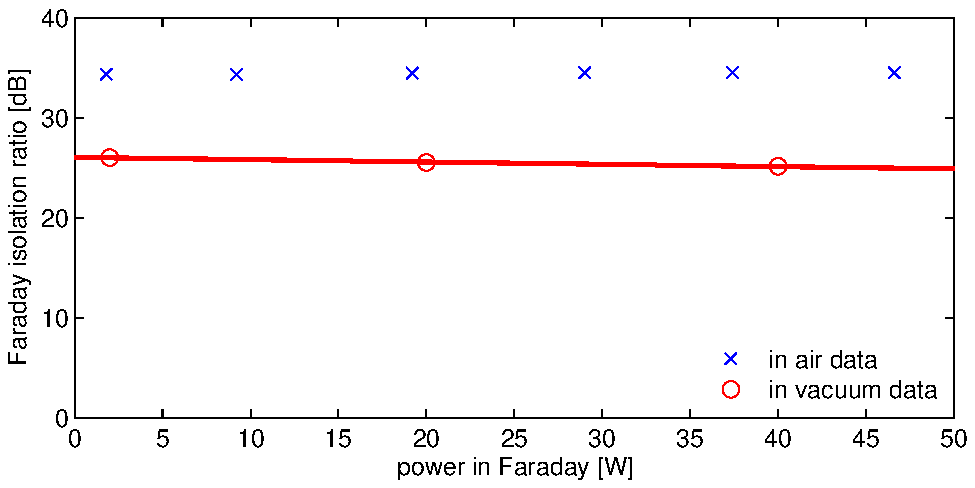
\includegraphics[width=1.0\columnwidth]{figures/FaradayIR.pdf}
\caption[Faraday isolator isolation ratio as measured in air and in
vacuum]{Faraday isolator isolation ratio as measured in air prior to
  installation and \emph{in situ} in vacuum. The isolation worsens by
  a factor of 6 upon placement of the Faraday in vacuum. The linear
  fits to the data show a constant in-air isolation ratio and an
  in-vacuum isolation ratio degradation of 0.02 dB/W.}
\label{fig:IR}
\end{centering}
\end{figure}

Figure \ref{fig:IR} shows our isolation ratio data. Most notably, we
observe an isolation decrease of a factor of six upon placing the
Faraday isolator in vacuum, a result consistent with that reported by
Ref. \citep{TheVIRGOCollaboration2008Invacuum}. In air the isolation
ratio is a constant 34.46 $\pm$ 0.04 dB from low power up to 47~W, and
in vacuum the isolation ratio is 26.5 dB at low power. The underlying
cause is the absence of cooling by air convection. If we attribute the
loss to the TGGs, then based on the change in TGG polarization
rotation angle necessary to produce the measured isolation drop of
8~dB and the temperature dependence of the TGG's Verdet constant, we
can put an upper limit of 11~K on the crystal temperature rise from
air to vacuum. Furthermore, a degradation of 0.02~dB/W is measured in
vacuum.

\subsection{Thermal Steering}
We measured the \emph{in situ} thermal angular drift of both the beam
transmitted through the mode cleaner and of the reflected beam from
the Faraday isolator with up to 25~W input power. Just as for the
isolation ratio measurement, we misaligned the interferometer arms so
that the input beam would be promptly reflected off of the recycling
mirror. The Faraday rotator was thus subjected to up to 50~W total
and the MC to 25~W. 

Pitch and yaw motion of the mode cleaner transmitted and
interferometer reflected beams were recorded using the quadrant
photodiode (QPD) on the Input Optics table and the RF alignment
detectors on the Interferometer Sensing and Control table, as seen in
Figure~\ref{fig:IOschematic}. There are no lenses between the MC waist
and its measurement QPD, so only the path length between the two were
needed to calibrate in radians the pitch and yaw signals on the
QPD. The interferometer reflected beam, however, passes through
several lenses. Thus, ray transfer matrices and the two alignment
detectors were necessary to extract the Faraday drift
calibration. Details of the calibration method are presented in
Appendix~\ref{sec:driftcal}.

Figure \ref{fig:drift} shows the calibrated beam steering data. The
angle of the beam out of the mode cleaner does not change measurably
as a function of input power in yaw (4.7~nrad/W) and changes by only
440~nrad/W in pitch. For the Faraday isolator, we record a beam drift
originating at the center of the Faraday rotator of 1.8~\microrad/W in
yaw and 3.2~\microrad/W in pitch. Therefore, when ramping the input
power up to 30~W during a full interferometer lock, the upper limit on
the drift experienced by the reflected beam is about 100
\microrad. This is a thirty-fold reduction with respect to the Initial
LIGO Faraday isolator and represents a fifth of the beam's divergence
angle, $\theta_{div}$~=~490 \microrad.

\begin{figure}
\begin{centering}
% \includegraphics[width=1.0\columnwidth]{figures/MC_FI_drift_labelled.pdf}
\subfigure[]{\includegraphics[width=1.0\columnwidth]{figures/forthesis_refldriftx10.pdf}}
\subfigure[]{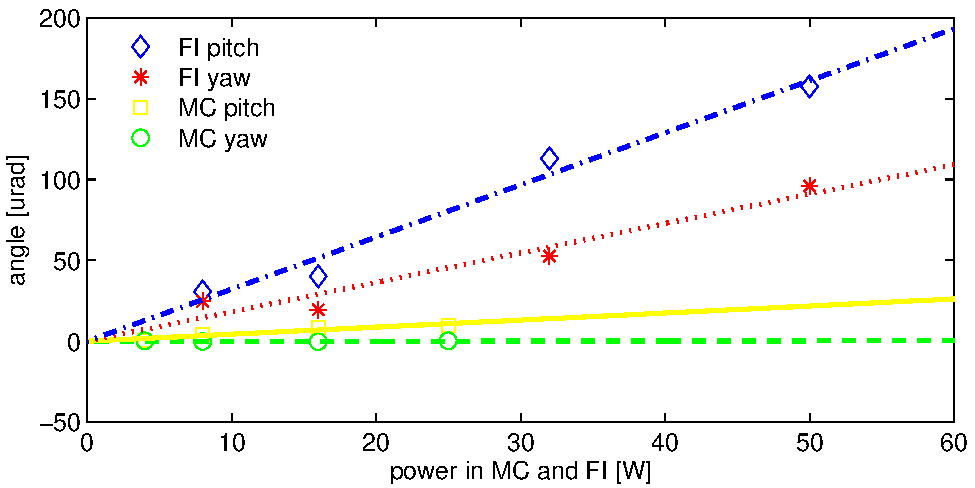
\includegraphics[width=1.0\columnwidth]{figures/alldrift.pdf}}
\caption[Mode cleaner and Faraday isolator thermal drift data.]{Mode
  cleaner and Faraday isolator thermal drift data. A) Angular motion
  of the beam at the MC waist and FI rotator as the input power is
  stepped. The beam is double-passed through the Faraday isolator, so
  it experiences twice the input power. B) Average beam angle per
  power level in the MC and FI. Linear fits to the data are also
  shown. The slopes for MC yaw, MC pitch, FI yaw, and FI pitch,
  respectively, are 0.0047, 0.44, 1.8, and 3.2 \microrad/W.}
\label{fig:drift}
\end{centering}
\end{figure}


\subsection{Thermal Lensing}
We measured the profiles of both the beam transmitted through the
mode cleaner and the reflected beam picked off by the Faraday isolator
at low ($\sim$~1~W) and high ($\sim$~25~W) input powers to assess the
degree of thermal lensing induced in the MC and FI. Again, we
misaligned the interferometer arms so that the input beam would be
promptly reflected off the recycling mirror. We picked off a fraction
of the reflected beam on the Interferometer Sensing and Control table
and of the mode cleaner transmitted beam on the Input Optics table
(refer to Figure \ref{fig:IOschematic}), placed lenses in each of their
paths, and measured the beam diameters at several locations on either
side of the waists created by the lenses. A change in the beam waist
size or position as a function of laser power indicates the presence
of a thermal lens.

\begin{figure}
\begin{centering}
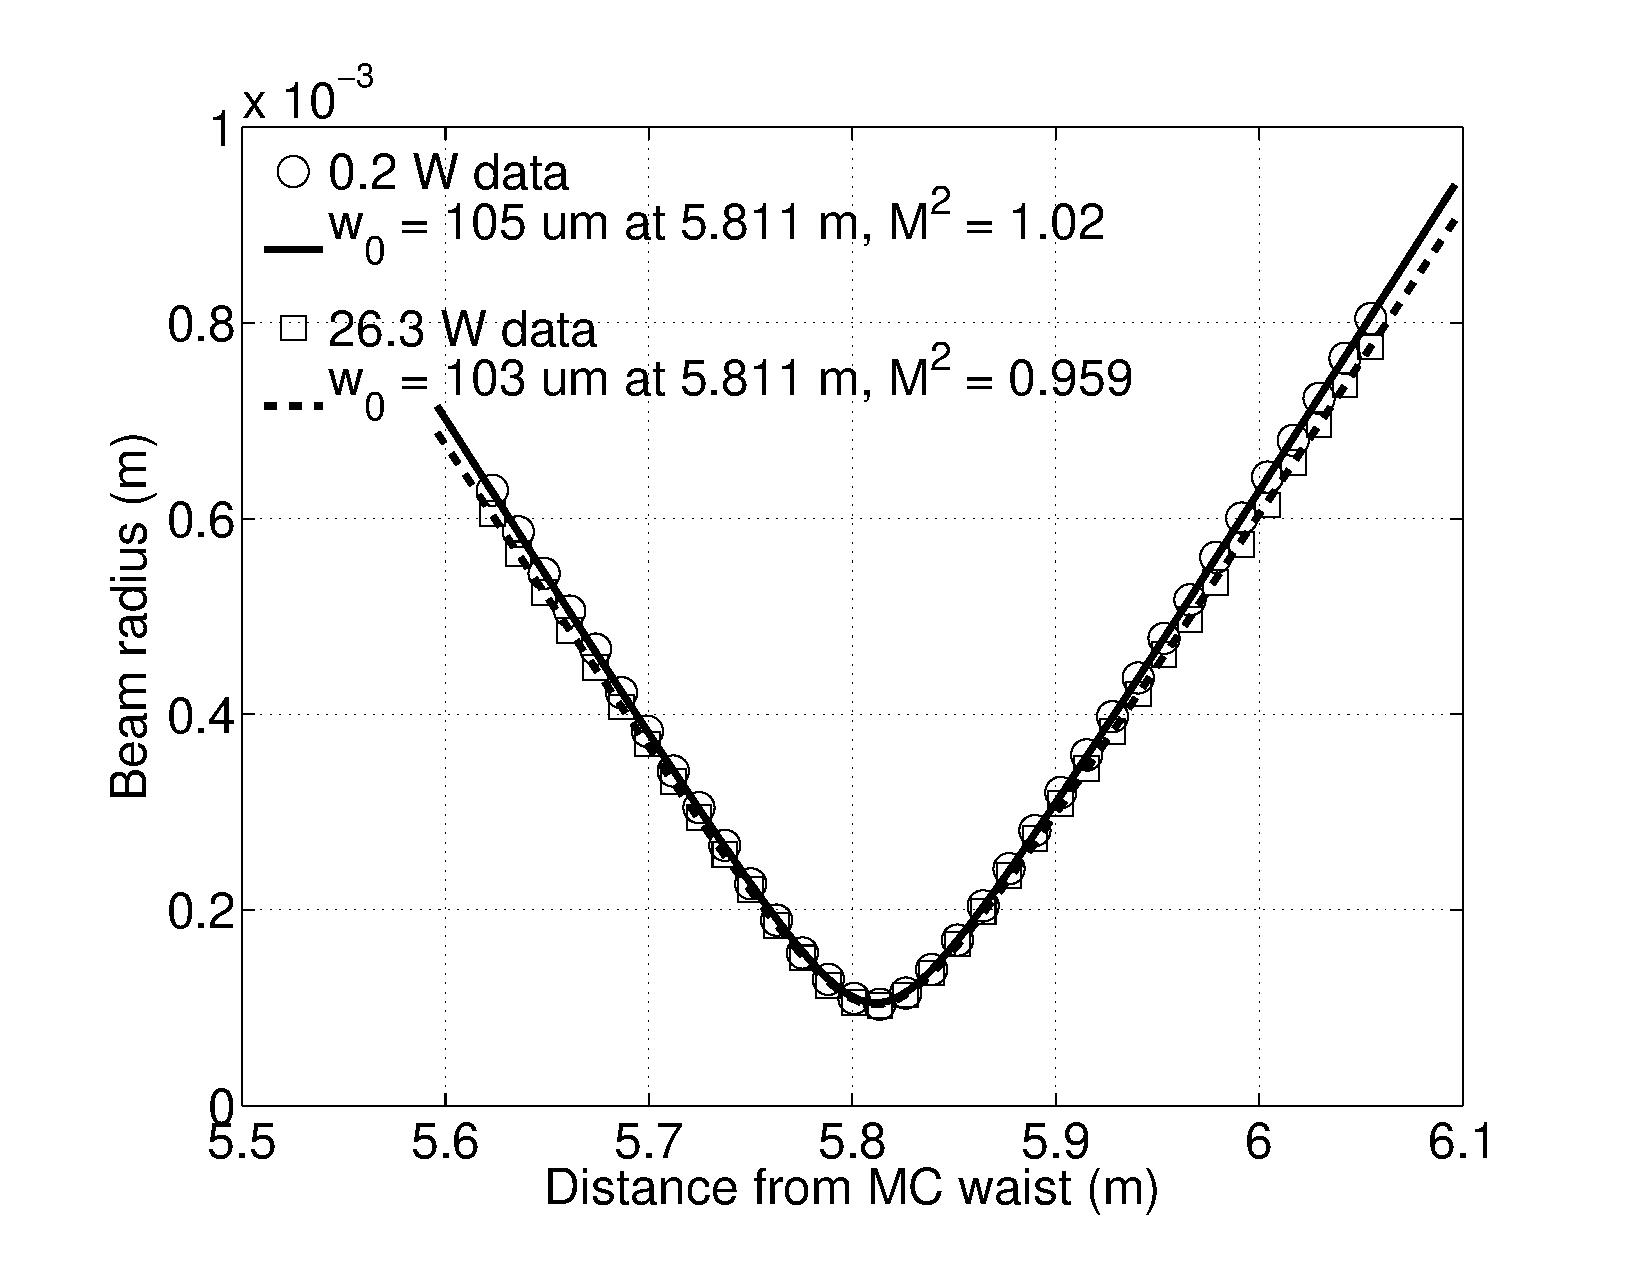
\includegraphics[width=1.0\columnwidth]{figures/MCTrans_datafit.pdf}
\caption[Profile at high and low powers of mode cleaner transmitted
beam]{Profile at high and low powers of a pick-off of the beam
  transmitted through the mode cleaner. The precision of the beam
  profiler is $\pm 5\%$. Within the error of the measurement, there
  are no obvious degradations.}
\label{fig:MC_lensing}
\end{centering}
\end{figure}

\begin{figure}
\begin{centering}
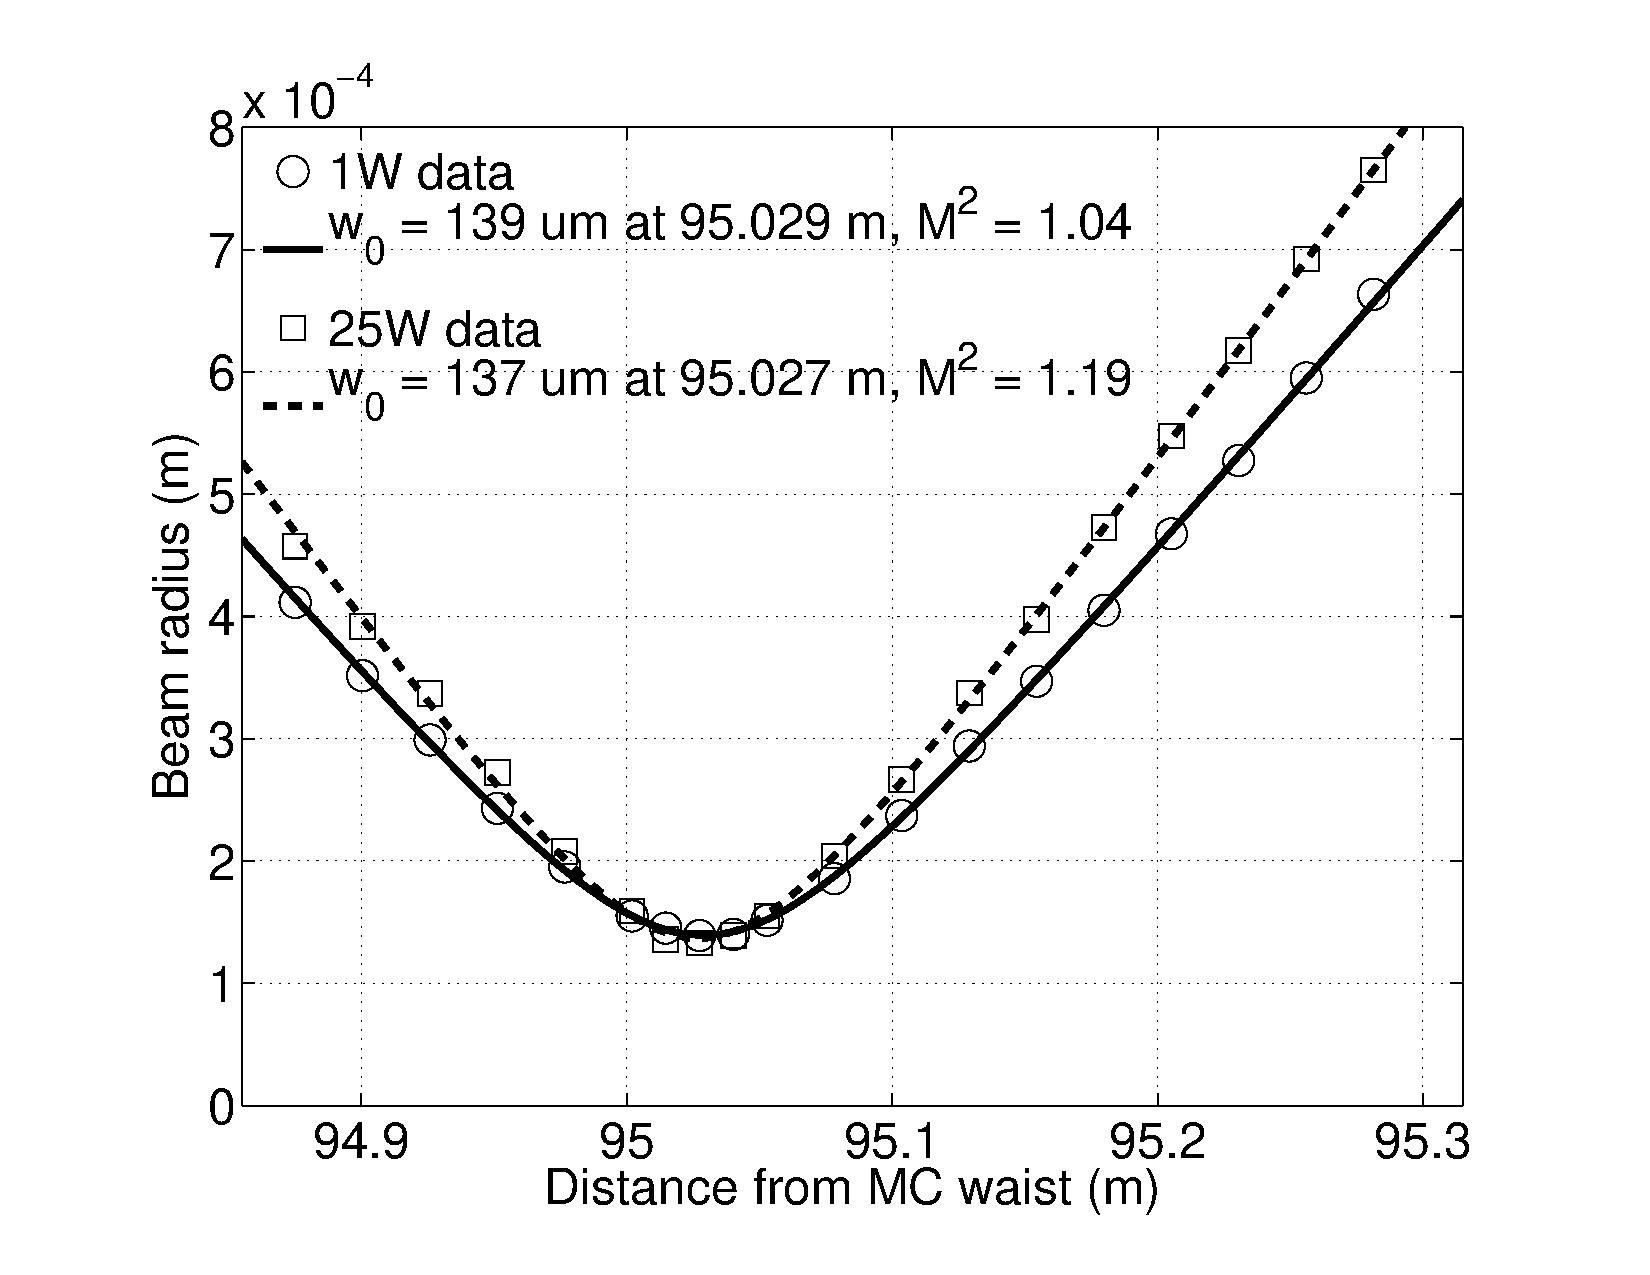
\includegraphics[width=1.0\columnwidth]{figures/REFL_datafit.pdf}
\caption[Faraday isolator thermal lensing data]{Faraday isolator
  thermal lensing data. With 25 W into the Faraday isolator
  (corresponding to 50 W in double pass), the beam has a steeper
  divergence than a pure TEM$_{00}$ beam, indicating the presence of
  higher order modes. Errors are $\pm 5.0\%$ for each data point.}
\label{fig:FI_lensing}
\end{centering}
\end{figure}

As seen in Figure~\ref{fig:MC_lensing} and Figure~\ref{fig:FI_lensing}, the
waists of the two sets of data are collocated: no thermal lens is
measured. For the Faraday isolator, the divergence of the low and high
power beams differs, indicating that the beam quality degrades with
power. The $M^2$ factor at 1~W is 1.04 indicating the beam is 
nearly perfectly a TEM$_{00}$ mode. At 25~W, $M^2$ increases to 1.19,
corresponding to increased higher-order-mode content. The percentage
of power in higher-order modes depends strongly on the mode order and
relative phases of the modes, and thus cannot be determined from this
measurement \citep{Kwee2007Laser}.

The results for the mode cleaner data are consistent with no thermal
lensing. The high and low power beam profiles are within each
other's error bars and well below our requirements. 

% We also measured the thermal lensing of the electro-optic modulator
% prior to its installation in Enhanced LIGO by comparing beam profiles
% of a 160~W beam with and without the EOM in its path. The data for
% both cross-sections of the beam is presented in
% Figure~\ref{fig:EOMlensing}. We observe no significant thermal lensing
% in the y-direction and a small effect in the x-direction. An upper
% limit for the thermal lens in the x-direction can be calculated to be
% greater than 4~m, which is 10 times larger than the Rayleigh range of
% the spatial mode. The mode matching degradation is therefore less
% than 1\%. Although a direct test for Advanced LIGO because of the
% power used, this measurement also serves to demonstrate the
% effectiveness of the EOM design for Enhanced LIGO powers.

% \begin{figure}
% \begin{centering}
% %\includegraphics[width=1.0\columnwidth]{figures/Picture1.png}
% \caption{EOM thermal lensing data.}
% \label{fig:EOMlensing}
% \end{centering}
% \end{figure}


\subsection{Mode-matching}
We measured the effectiveness of the mode-matching telescope by taking
the ratio of power at the reflected port when all of the
interferometer cavities are on resonance to the power in the reflected
beam when the cavities are unlocked. Since the impedance matching is
near perfect, all light at the reflected port during interferometer
lock is attributable to a mode mismatch. Initially, anywhere
between 10\% and 17\% of the light was rejected by the cavity due to
poor, power-dependent mode matching.  After translating the
mode-matching telescope mirrors during a vacuum chamber incursion and
upgrading the other IO components, the ratio we measured was 8\%
independent of input power. The MMT succeeds at coupling 92\% of the
light into the interferometer at all times, marking both an
improvement in MMT mirror placement and success in eliminating
measurable thermal issues. Appendix~\ref{sec:MM} details of the
mode-matching measurement.


\section{Implications for Advanced LIGO}
\label{sec:aLIGO}
As with other Advanced LIGO interferometer components, Enhanced LIGO
served as a technology demonstrator for the Advanced LIGO Input
Optics, albeit at lower laser powers than will be used there. The
performance of the Enhanced LIGO Input Optics components, at 20~W of
input power allows us to infer their performance in Advanced LIGO.
The requirements for the Advanced LIGO Input Optics demand are for
similar performance to Enhanced LIGO, but with almost 8 times the
laser power.

The Enhanced LIGO electro-optic modulator showed no thermal lensing,
degraded transmission, nor damage in over 1 million hours of sustained
operation at 30~W of laser power. Measurements of the thermal lensing
in RTP at powers up to 160 W show a relative power loss of $< 0.4\%$,
indicating that thermal lensing should be negligible in Advanced LIGO.
Peak irradiances in the EOM will be approximately four times that of
Enhanced LIGO (a 45\% larger beam diameter will somewhat offset the
increased power).  Testing of RTP at 10 times the expected Advanced
LIGO irradiance over 100~hours show no signs of damage or degraded
transmission.

The mode cleaner showed no measurable change in operational state as a
function of input power.  This bodes well for the Advanced LIGO mode
cleaner.  Compared with the Enhanced LIGO mode cleaner, the Advanced
LIGO mode cleaner is designed with a lower finesse (520) than Initial
LIGO (1280).  For 150~W input power, the Advanced LIGO mode cleaner
will operate with 3 times greater stored power than Initial LIGO.  The
corresponding peak irradiance is 400~kW/m$^2$, well below the
continuous wave coating damage threshold.  Absorption in the Advanced
LIGO mode cleaner mirror optical coatings has been measured at
0.5~ppm, roughly four times less than the best mirror coating
absorption in Enhanced LIGO, so the expected thermal loading due to
coating absorption should be reduced in Advanced LIGO.  The larger
Advanced LIGO mode cleaner mirror substrates and higher input powers
result in a significantly higher contribution to bulk absorption,
roughly 20 times Enhanced LIGO, however the expected thermal lensing
leads to small change ($< 0.5 \%$) in the output mode
\citep{Arain2007Note}.

The Enhanced LIGO data obtained from the FI allows us to make several
predictions about how it will perform in Advanced LIGO.  The measured
isolation ratio decrease of 0.02~dB/W will result in a loss of 3~dB
for a 150~W power level expected for Advanced LIGO relative to its
cold state.  However, the Advanced LIGO FI will employ an \emph{in
  situ} adjustable half wave plate which will allow for a partial
restoration of the isolation ratio. In addition, a new FI scheme to
better compensate for thermal depolarization and thus yield higher
isolation ratios may be implemented
\cite{Snetkov2011Compensation}. The maximum thermally induced angular
steering expected is 480 \micro rad (using a drift rate of
3.2~\microrad/W), approximately equal to the beam divergence
angle. This has some implications for the Advanced LIGO length and
alignment sensing and control system, as the reflected FI beam is used
as a sensing beam. Operation of Advanced LIGO at high powers will
likely require the use of a beam stabilization servo to lock the
position of the reflected beam on the sensing photodiodes.  Although
no measurable thermal lensing was observed (no change in the beam
waist size or position), the measured presence of higher order modes
in the FI at high powers is suggestive of imperfect thermal lens
compensation by the DKDP.  This fault potentially can be reduced by a
careful selection of the thickness of the DKDP to better match the
absorbed power in the TGG crystals.

\section{Summary}
\label{sec:summary}
In summary, we have presented a comprehensive investigation of the
Enhanced LIGO Input Optics, including the function, design, and
performance of the IO.  Several improvements to the design and
implementation of the Enhanced LIGO IO over the Initial LIGO IO have
lead to improved optical efficiency and coupling to the main
interferometer through a substantial reduction in thermo-optical
effects in the major IO optical components, including the
electro-optic modulators, mode cleaner, and Faraday isolator.  The IO
performance in Enhanced LIGO enables us to infer its performance in
Advanced LIGO, and indicates that high power interferometry will be
possible without severe thermal effects.


% \textcolor{blue}{from Guido: summary of the improvements due to the
%   changes in the IO. More power, better shot noise sensitivity,
%   better range, better upper limits, lessons learned for aLIGO
%   (summary like, the details should be in the previous
%   subsections). Make it glorious and complain that other subsystems
%   (TCS) wasn't able to handle the power. Otherwise this becomes very
%   technical and boring.}

% \section{Radiation pressure in MC}
% \textcolor{blue}{Maybe write up April 4, 2009 notebook derivation of
%   radiation pressure length spring in MC. Also, Rana has a noise
%   budget elog entry April 3, 2009.}

\chapter{Input Optics Design and Characterization}

\section{Function of the Input Optics}
\label{sec:role}

\begin{figure*}
\begin{centering}
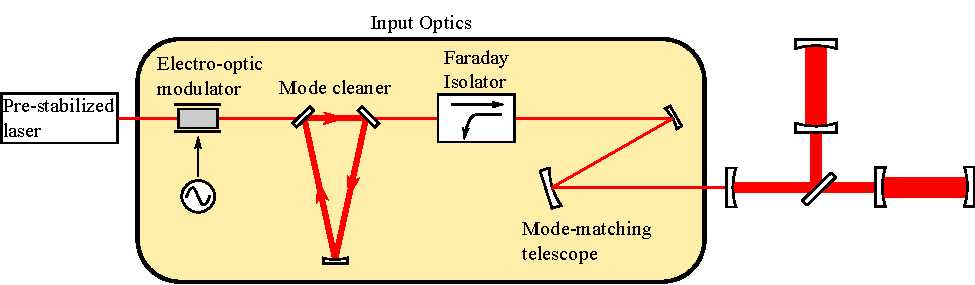
\includegraphics{figures/InputOpticsBlock_thesis.pdf}
\caption[Block diagram of the Input Optics subsystem.]{Block diagram
  of the Input Optics subsystem. The IO is located between the
  pre-stabilized laser and the recycling mirror and consists of four
  components: electro-optic modulator, mode cleaner, Farday isolator,
  and mode-matching telescope. The electro-optic modulator is the only
  IO component outside of the vacuum system. Diagram is not to scale.}
\label{fig:IOblock}
\end{centering}
\end{figure*}

The Input Optics is one of the primary subsystems of the LIGO
interferometers. Its purpose is to deliver an aligned, spatially
pure, mode-matched beam with phase-modulation sidebands to the
power-recycled Fabry-Perot Michelson interferometer. The IO also
prevents the backscattering of light into the laser and distributes
the control sidebands reflected from the interferometer (designated
the \emph{reflected port}) to photodiodes for sensing and controlling
the length and alignment of the interferometer. In addition, the IO
provides an intermediate level of frequency stabilization and must
have high overall optical efficiency. It must perform these functions
without limiting the strain sensitivity of the LIGO interferometer.
Finally, it must operate robustly and continuously over years of
operation. The conceptual design is found in
Ref.~\citep{Camp1996InputOutput}.

As shown in Fig.~\ref{fig:IOblock}, the Input Optics subsystem
consists of four components located between the pre-stabilized laser
and the power recycling mirror:
\begin{itemize}
\item electro-optic modulator (EOM) \vspace{-10 pt}
\item mode cleaner cavity (MC) \vspace{-10 pt}
\item Faraday isolator (FI) \vspace{-10 pt}
\item mode-matching telescope (MMT)
\end{itemize}
Each element is a common building block of many optical experiments
and not unique to LIGO. However, their roles specific to the
successful operation of interferometry for gravitational-wave
detection are of interest and demand further attention. Here, we
briefly review the purpose of each of the Input Optics components;
further details about the design requirements are in
Ref.~\citep{Camp1997Input}.




\subsection{Electro-optic Modulator} 
The Length Sensing and Control (LSC) and Angular Sensing and Control
(ASC) subsystems require phase modulation of the laser light at RF
frequencies. This modulation is produced by an EOM, generating
sidebands of the laser light which act as references against which
interferometer length and angle changes are measured
\citep{Fritschel2001Readout}. The sideband light must be either
resonant only in the recycling cavity or not resonant in the
interferometer at all. The sidebands must be offset from the carrier
by integer multiples of the mode cleaner free spectral range so that
neither MC length fluctations nor phase modulation of the sidebands
(due to phase noise of the RF oscillator) are converted to amplitude modulation.


\subsection{Mode Cleaner}
Stably aligned cavities, limited junk light, and a frequency and
amplitude stabilized laser are key features of any ultra sensitive
laser interferometer. The mode cleaner, at the heart of the IO, plays
a major role to this effect.

A three-mirror triangular ring cavity, the mode cleaner suppresses laser output not in
the fundamental TEM$_{00}$ mode, serving two major purposes. It enables the robustness of the
ASC since higher order modes would otherwise contaminate the angular sensing
signals of the interferometer. Also, all non-TEM$_{00}$ light on the
length sensing photodiodes, including those used for the GW readout,
contributes shot noise but not signal and therefore diminishes the signal to
noise ratio. The mode cleaner is thus largely responsible for achieving an aligned,
minimally shot-noise-limited interferometer. 

The mode cleaner also plays an active role in laser frequency
stabilization \citep{Zucker2002H1}. A frequency-stabilized laser is
necessary for ensuring that the signal at the anti-symmetric port is
due to arm length fluctuations rather than laser frequency
fluctuations. In principle, the two-arm geometry of LIGO facilitates
this distinction, but imbalances between the arms allow frequency
noise to couple into the gravitational wave channel. At low
frequencies ($<$~100 Hz) the average interferometer arm length drives
the mode cleaner length, which in turn adjusts the laser frequency. At
high frequencies (up to 20~kHz), the common arm length adds an
electronic offset to the MC error point, also resulting in a shift of
the laser frequency. As a result, the light transmitted through the MC
is matched to the very quiet arms.
 
The mode cleaner acts as a passive laser amplitude fluctuation
filter. Laser power fluctuations that couple to the antisymmetric port
cause noise in the GW readout.  The mode cleaner suppresses laser
amplitude noise above its pole frequency of about 4500~Hz. In
addition, the MC passively supresses beam jitter at frequencies above
10~Hz.


\subsection{Faraday Isolator}
Faraday isolators are four-port optical devices which utilize the
Faraday effect to allow for non-reciprocal polarization switching of
laser beams.  Any reflected light from the interferometer due to
impedance mismatch, mode mismatch, non-resonant sidebands, or signal
needs to be diverted to protect the laser from back propagating light,
which can introduce amplitude and phase noise.  This diversion of the
reflected light is also necessary for extracting length and angular
information about the interferometer's cavities. The Faraday isolator
accomplishes both needs.


\subsection{Mode-matching Telescope}
The lowest order mode cleaner and arm cavity spatial eigenmodes need
to be matched for maximal power buildup in the interferometer. The
mode-matching telescope is a set of three suspended concave mirrors
between the mode cleaner and interferometer that expand the beam from
a radius of 1.6~mm at the mode cleaner waist to a radius of 37~mm at
the recycling mirror.  The MMT should play a passive role by
delivering properly shaped light to the interferometer without
introducing beam jitter or any significant aberration that can reduce
mode coupling.




\section{Thermal Problems in Initial LIGO}
\label{sec:problems}
The Initial LIGO interferometers were equipped with a 10~W laser, yet
operated with only 7~W input power to the interferometer due to
power-related problems with other subsystems. The EOM was located in
the 10~W beam and the other components experienced anywhere up to 7~W
power. The 7~W operational limit was not due to the failure of the
Input Optics; however, many aspects of the IO performance did degrade
with power.

One of the primary problems of the Initial LIGO Input Optics
\citep{Adhikari1998Input} was thermal deflection of the back
propagating beam due to thermally-induced refractive index gradients
in the Faraday isolator. A significant beam drift between the
interferometer's locked and unlocked states led to clipping of the
reflected beam on the photodiodes used for length and alignment
contro. Our measurements determined a deflection of approximately
100~\microrad/W in the FI.  This was mitigated at the time by the
design and implementation of an active beam steering servo on the beam
rejected by the isolator.

There were also known limits to the power the IO could sustain.
Thermal lensing in the Faraday isolator optics would start to
significantly alter the beam mode at powers greater than 10~W, leading
to a several percent reduction in mode matching to the interferometer
\citep{UFLIGOGroup2006Upgrading}.  Additionally, the absorptive FI
elements would create thermal birefringence, degrading the optical
efficiency and isolation ratio with power
\citep{Khazanov1999Investigation}.  The Initial LIGO New Focus
electro-optic modulators had an operational power limit of around
10~W. There was a high risk of damage to the crystals under the stress
of the 0.4~mm radius beam. Also, anisotropic thermal lensing with
focal lengths as severe as 3.3~m at 10~W made the EOMs unsuitable for
much higher power. Finally, the mode cleaner mirrors exhibited high
absorption (as much as 24 ppm per mirror), enough that thermal lensing
of the MC optics at Enhanced LIGO powers would induce higher order
modal frequency degeneracy and result in a power-dependent mode
mismatch into the interferometer \citep{Bullington2008Modal,
  Arain2007Note}. In fact, as input power increased from 1~W to 7~W
the mode matching decreased from 90\% to 83\%.

In addition to the thermal limitations of the Initial LIGO IO, optical
efficiency in delivering light from the laser into the interferometer
was not optimal. Of the light entering the Input Optics chain, only
60\% remained by the time it reached the power recycling
mirror. Moreover, since only 90\% at best of the light at the
recycling mirror was coupled into the arm cavity mode, room was left
for improvement in the implementation of the MMT.


\begin{sidewaysfigure}
\begin{centering}
\includegraphics[width=1.0\textwidth]{figures/iopaperIO_withHam2.pdf}
\caption[Enhanced LIGO Input Optics optical and sensing
  configuration]{Enhanced LIGO Input Optics optical and sensing
  configuration. The HAM1 (horizontal access module) vacuum chamber is
  featured in the center, with locations of all major optics
  superimposed. HAM2 is shown on the right, with its components. These
  tables are separated by 12~m. The primary beam path, beginning at
  the pre-stabilized laser and going to the power recycling mirror, is
  shown in red as a solid line, and auxiliary beams are different
  colors and dotted. The MMTs, MCs, and steering mirror (SM) are
  suspended; all other optics are fixed to the seismically isolated
  table. The laser and sensing and diagnostic photodiodes are on
  in-air tables.}
\label{fig:IOschematic}
\end{centering}
\end{sidewaysfigure}

\section{Enhanced LIGO Input Optics Design}
\label{sec:design}
The Enhanced LIGO Input Optics design addressed the thermal effects
that compromised the performance of Initial LIGO, and accommodated up
to four times the power of Initial LIGO. Also, the design was a
prototype for handling the 165~W laser planned for Advanced
LIGO. Since the adverse thermal properties of the Initial LIGO IO
(beam drift, birefringence, and lensing) are all attributable
primarily to absorption of laser light by the optical elements, the
primary design consideration was finding optics with excellent
thermo-optical properties \citep{UFLIGOGroup2006Upgrading}. Both the
EOM and the FI were replaced for Enhanced LIGO. Only minor changes
were made to the MC and MMT. A detailed layout of the Enhanced LIGO IO
is shown in Figure \ref{fig:IOschematic}.


\subsection{Electro-optic Modulator Design}
We replaced the commercially-made New Focus 4003 resonant phase
modulator of Initial LIGO with an EOM design and construction of our
own. Both a new crystal choice and architectural design change allow
for superior performance.

The Enhanced LIGO EOM design uses a crystal of rubidium titanyl
phosphate (RTP), which has at most 1/10 the absorption coefficient at
1064 nm of the lithium niobate (LiNbO$_3$) crystal from Initial
LIGO. At 200~W the RTP should produce a thermal lens of 200 m and
higher order mode content of less than 1\%, compared to the 3.3~m lens
the LiNbO$_3$ produces at 10~W. The RTP has a minimal risk of damage,
since it has both twice the damage threshold of LiNbO$_3$ and is
subjected to a beam twice the size of that in Initial LIGO. RTP and
LiNbO$_3$ have similar electro-optic coefficients. Also, RTP's $dn/dT$
anisotropy is 50\% smaller. Table \ref{tab:EOMcrystals} compares the
properties of most interest of the two crystals.

\begin{table*}
\centering
\caption[Comparison of selected properties of the Initial and Enhanced
 LIGO EOM crystals]{Comparison of selected properties of the Initial and Enhanced
 LIGO EOM crystals, LiNbO$_3$ and RTP, respectively. RTP was
 preferred for Enhanced LIGO because of its lower absorption,
 superior thermal properties, and similar 
 electro-optic properties \citep{UFLIGOGroup2006Upgrading}.}  
\begin{tabular}{l l l l}
\hline
 & units & LiNbO$_3$ & RTP \\
\hline
damage threshold & MW/cm$^2$ & 280 & $>600$ \\
absorption coeff. at 1064 nm & cm$^{-1}$ & $< 0.005$ & $< 0.0005$ \\
electro-optic coeff. ($n_z^3 r_{33}$) & pm/V & 306 & 239 \\
$dn_y/dT$ & 10$^{-6}$/K & 5.4 & 2.79 \\
$dn_z/dT$ & 10$^{-6}$/K & 37.9 & 9.24 \\
\hline
\end{tabular}
\label{tab:EOMcrystals}
\end{table*}

We procured the RTP crystals from Raicol and packaged them into
specially designed custom built modulators. The crystal dimensions are
$4 \times 4 \times 40$ mm and their faces are wedged by $2.85^\circ$
and anti-reflection (AR) coated. The wedge serves to separate the
polarizations and prevents an etalon effect, resulting in a
suppression of amplitude modulation. Only one crystal is used in the
EOM in order to reduce the number of surface reflections. Three
separate pairs of electrodes, each with its own resonant LC circuit,
are placed across the crystal in series, producing the three required
sets of RF sidebands: 24.5~MHz, 33.3~MHZ and 61.2~MHz. A diagram is
shown in Fig. \ref{fig:EOM}. Reference
\citep{Quetschke2008ElectroOptic} contains further details about the
modulator architecture.

\begin{figure}
\begin{centering}
  \subfigure[A single RTP crystal is sandwiched between three sets of
  electrodes that apply three different modulation frequencies. The
  wedged ends of the crystal separate the polarizations of the
  light. The p-polarized light is used in the
  interferometer.]{\includegraphics{figures/EOMthesis.pdf}}
  \subfigure[A schematic for each of the three impedance matching
  circuits of the EOM. For the three sets of electrodes, each of which
  creates its own $C_{crystal}$, a capacitor is placed parallel to the
  LC circuit formed by the crystal and a hand-wound inductor.  The
  circuits provide 50~$\Omega$ input impedance on resonance and are
  housed in a separate box from the
  crystal.]{\includegraphics{figures/EOMcircuit_thesis.pdf}}
\caption[Electro-optic modulator design]{Electro-optic modulator
  design.}
\label{fig:EOM}
\end{centering}
\end{figure}

\subsection{Mode Cleaner Design}
The mode cleaner is a suspended 12.2~m long triangular ring cavity
with finesse $\mathcal{F}$=1282 and free spectral range of
12.243~MHz. The three mirror architecture was selected over the
standard two mirror linear filter cavity because it acts as a
polarization filter and because it eliminates direct path back
propagation to the laser \citep{Raab1992Estimation}. A pick-off of the
reflected beam is naturally facilitated for use in generating control
signals. A potential downside to the three mirror design is the
introduction of astigmatism, but this effect is negligible due to the
small opening angle of the mode cleaner. 

The MC has a round-trip length of 24.5~m. The beam waist has a radius of
1.63~mm and is located between two 45$^\circ$ flat mirrors, MC1 and
MC3 (see Fig. \ref{fig:IOschematic}). A concave third mirror, MC2,
with an 18.15~m radius of curvature forms the far point of the mode
cleaner's isoceles triangle shape. The power stored in the MC is 408
times the amount coupled in, equivalent to about 2.7~kW in Initial
LIGO and at most 11~kW for Enhanced LIGO. The peak irradiances are
32~kW/cm$^2$ and 132~kW/cm$^2$ for Initial LIGO and Enhanced LIGO,
respectively. The scattering losses of each mirror due to measured
surface microroughness are 22~ppm.

The mode cleaner mirrors are 75 mm in diameter and 25 mm thick. The
substrate material is fused silica and the mirror coating is made of
alternating layers of silica and tantala. In order to reduce the
absorption of heat in these materials and therefore improve the
transmission and modal quality of the beam in the mode cleaner, we
removed particulate by drag wiping the surface of the MC mirrors with
methanol and optical tissues. The mode cleaner was otherwise identical
to that in Initial LIGO.



\subsection{Faraday Isolator Design}
The Enhanced LIGO Faraday isolator design required not only the use of
low absorption optics, but additional design choices to mitigate any
residual thermal lensing and birefringence. In additon, trade-offs
between optical throughput in the forward direction, optical isolation
in the backwards direction, and feasibility of physical access of the
return beam for signal use were considered. The result is that the
Enhanced LIGO Faraday isolator needed a completely new architecture
and new optics compared to both the Initial LIGO FI and commercially
available isolators.

Figure \ref{fig:FI} shows a schematic of the Enhanced LIGO Faraday
Isolator. It begins and ends with low absorption calcite wedge
polarizers (CWP). Between the CWPs is a thin film polarizer (TFP), a
deuterated potassium dihydrogen phosphate (DKDP) element, a half-wave
plate (HWP), and a Faraday rotator. The rotator is made of two low
absorption terbium gallium garnet (TGG) crystals sandwiching a quartz
rotator (QR) inside a 7-disc magnet with a maximum field strength of
1.16~T. The forward propagating beam upon passing through the TGG, QR,
TGG, and HWP elements is rotated by $+22.5^\circ - 67.5^\circ +
22.5^\circ + 22.5^\circ = 0^\circ$. In the reverse direction, the
rotation through HWP, TGG, QR, TGG is $-22.5^\circ + 22.5^\circ +
67.5^\circ + 22.5^\circ = 90^\circ$. The TGG crystals are
non-reciprocal devices while the QR is reciprocal.

\begin{figure}
\begin{centering}
\subfigure{\includegraphics[width=0.9\columnwidth]{figures/FI_cropped2.jpg}}
\subfigure{\includegraphics{figures/FI_thesis.pdf}}
\caption[Faraday isolator photograph and schematic.]{Faraday isolator
  photograph and schematic. The Faraday isolator preserves the
  polarization of the light in the forward-going direction and rotates
  it by 90 degrees in the reverse direction. Light from the MC enters
  from the left and exits at the right towards the interferometer. It
  is ideally p-polarized, but any s-polarization contamination is
  promptly diverted $\sim 10$ mrad by the CWP and then reflected by
  the TFP and dumped. The p-polarized reflected beam from the
  interferometer enters from the right and is rotated to s-polarized
  light which is picked-off by the TFP and sent to the Interferometer
  Sensing and Control (ISC) table. Any imperfections in the Faraday
  rotation of the interferometer return beam results in p-polarized
  light traveling backwards along the original input path.}
\label{fig:FI}
\end{centering}
\end{figure}

\subsubsection{Thermal birefringence} 
Thermal birefringence is addressed in the Faraday rotator by the use
of the two TGG crystals and one quartz rotator rather than the typical
single TGG \citep{Khazanov2000Suppression}.  In this configuration, any
thermal polarization distortions that the beam experiences while
passing through the first TGG rotator will be partially undone upon
passing through the second. \textcolor{blue}{(Add sentence of further
  explanation.)} The multiple elements in the magnet required a larger
magnetic field than in Initial LIGO and a Faraday rotator housing that
is 15.5~cm in diameter by 16.1~cm long. The TGG diameter is 20~mm.

\subsubsection{Thermal lensing}  
Thermal lensing in the Faraday isolator is addressed by including
DKDP, a negative $dn/dT$ material, in the beam path. Absorption of
light in the DKDP results in a de-focusing of the beam, which
partially compensates for the thermal focusing induced by absorption
in the TGGs \citep{Mueller2002Method, Khazanov2004Compensation}.  The
optical path length (thickness) of the DKDP is chosen to slightly
over-compensate the positive thermal lens induced in the TGG crystals,
anticipating other positive thermal lenses in the system.

\subsubsection{Polarizers}  
The polarizers used (two CWPs and one TFP) each offer advantages and
disadvantages related to optical efficiency in the forward-propagating
direction, optical isolation in the reflected direction, and thermal
beam drift. The CWPs have very high extinction ratios ($>10^5$) and
high transmission ($>$ 99\%) contributing to good optical efficiency
and isolation performance. However, the angle separating the exiting
orthogonal polarizations of light is very small, on the order of 10
mrad. This requires relatively large distances to pick off the beams
needed for interferometer sensing and control. In addition, thermally
induced index of refraction gradients due to the 4.95$^{\circ}$ wedge
angle of the CWPs result in thermal drift. However, the CWPs for the
Enhanced LIGO Faraday have a measured low absorption of 0.0013
cm$^{-1}$
%(from eLIGO wiki) 
with an expected thermal lens of 60~m at 30~W and drift of less than
1.3 $\mu$rad/W \citep{UFLIGOGroup2006Upgrading}.

The advantages of the thin film polarizer over the calcite wedge
polarizer are that it exhibits negligible thermal drift when compared
with CWPs and it operates at the Brewster angle of 55$^\circ$, thus
diverting the return beam in an easily accessible way. However, the
TFP has a lower transmission than the CWP, about 96\%, and an
extinction ratio of only 10$^3$.

Thus, the combination of CWPs and a TFP combines the best of each to
provide a high extinction ratio (from the CWPs) and ease of reflected
beam extraction (from the TFP). The downsides that remain when using
both polarizers are that there is still some thermal drift from the
CWPs. Also the transmission is reduced due to the TFP and to the fact
that there are 16 surfaces from which light can scatter.

\subsubsection{Heat conduction}
\label{sec:heatconduction}
Faraday isolators operating in a vacuum environment suffer from
increased heating with respect to those operating in air. Convective
cooling at the faces of the optical components is no longer an
effective heat removal channel, so proper heat sinking is essential to
minimize thermal lensing and depolarization. It has been shown that
Faraday isolators carefully aligned in air can experience a dramatic
reduction in isolation ratio ($>$ 10-15 dB) when placed in vacuum
\citep{TheVIRGOCollaboration2008Invacuum}. The dominant cause is the
coupling of the photoelastic effect to the temperature gradient
induced by laser beam absorption. Also of importance is the
temperature dependence of the Verdet constant--different spatial parts
of the beam experience different linear polarizations in the presence
of a temperature gradient.

To improve heat conduction away from the Faraday rotator optical
components, we designed housing for the TGG and quartz crystals that
provided improved heat sinking to the Faraday rotator. We also wrapped
the TGGs with indium foil as pictured in Fig. \ref{fig:TGG} to improve
contact with the housing, and we cushioned the DKDP and the HWP with
indium wire in their aluminum holders. This has the additional effect
of avoiding the development of thermal stresses in the crystals, an
especially important consideration for the very fragile DKDP.

\begin{figure}
\begin{centering}
\includegraphics{figures/TGG_scaled.jpg}
  \caption[Photo indium-wrapped TGG crystal]{Photo of TGG crystal
    with indium foil wrapping.}
\label{fig:TGG}
\end{centering}
\end{figure}


\subsection{Mode-matching Telescope Design}
% from May 31, 2007 elog
The mode matching into the interferometer (at Livingston) was measured
to be at best 90\% in Initial LIGO. Because of the stringent
requirements placed on the LIGO vacuum system to reduce phase noise
through scattering by residual gas, standard opto-mechanical
translators are not permitted in the vacuum; it is therefore not
possible to physically move the mode matching telescope mirrors while
operating the interferometer. Through a combination of needing to move
the MMTs in order to fit the new Faraday isolator on the in-vacuum
optics table and additional measurements and models to determine how
to improve the coupling, a new set of MMT positions was chosen for
Enhanced LIGO. Fundamental design considerations are discussed in
Ref. \citep{Delker1997Design}.



\section{Performance of the Enhanced LIGO Input Optics}
\label{sec:performance}
The most convincing figure of merit for the Input Optics performance
is that the Enhanced LIGO interferometers achieved low-noise operation
with 20 W input power without thermal issues from the
IO. Additionally, the Input Optics were operated successfully up to
the available 30 W of power.  (Instabilities with other interferometer
subsystems limited the Enhanced LIGO science run operation to 20~W.)
We present in this section detailed measurements of the Input Optics
performance during Enhanced LIGO. Specific measurements and results
presented in figures and the text come from Livingston; performance at
Hanford was similar and is included in tables summarizing the results.



\subsection{Optical efficiency}
The optical efficiency of the Enhanced LIGO Input Optics from EOM to
recycling mirror was 75\%, a marked improvement over the approximate
60\% that was measured for Initial LIGO. A substantial part of the
improvement came from the discovery and subsequent correction of a
6.5\% loss at the second of the in-vacuum steering mirrors directing
light into the MC (refer to Fig. \ref{fig:IOschematic}). A 45$^\circ$
reflecting mirror had been used for a beam with an 8$^\circ$ angle of
incidence. Losses attributable to the mode cleaner and Faraday
isolator are described in the following sections. A summary of the IO
power budget is found in Table \ref{tab:pwrbudget}.

\begin{table}
\centering
\caption[Enhanced LIGO Input Optics power budget.]{Enhanced LIGO Input
  Optics power budget. Errors are $\pm 1\%$, except for the TFP loss
  whose error is $\pm 0.1\%$. The 
  composite mode cleaner transmission is the percentage of power after the MC to
  before the MC and is the product of the MC visibility and
  transmission. Initial LIGO values,
  where known, are included in parentheses and have errors of several percent.}
\begin{tabular}{l l l}
\hline
 & Livingston & Hanford \\
\hline
Mode cleaner visibility & 92\% & 97\% \\
Mode cleaner transmission & 88\% & 90\% \\
Composite MC transmission & 81\% (72\%) & 87\% \\
Faraday transmission &       93\% (86\%) & 94\% (86\%) \\
\hspace{0.5cm} - Thin film polarizer loss & 4.0\% & 2.7\% \\ 
IO efficiency (PSL to RM) & 75\% (60\%) & 82\% \\
\hline
\end{tabular}
\label{tab:pwrbudget}
\end{table}


\subsubsection{Mode cleaner losses} 
The mode cleaner was the greatest single source of power loss in both
Initial and Enhanced LIGO. The mode cleaner visibility, defined here as
\begin{equation}
\mbox{visibility} = 1 - \frac{P_{reflected}}{P_{in}},
\end{equation}
the ratio of the amount of light coupled into the MC to the amount
impinging the mode cleaner input mirror, was 92\%. Losses are the result of higher
order mode content and mode mismatch into the MC. The visibility was
constant within 0.04\% up to 30~W input power at both sites, providing a positive
indication that thermal aberrations in the mode cleaner were
negligible. 

Of the light coupled into the mode cleaner, 88\% was transmitted,
corresponding to an average loss of 98 ppm per mirror. Based on the
mirrors' known surface micro-roughness, the scatter loss is expected
to be 22 ppm/mirror. Part of the discrepancy between expectation and
measurement was determined to come from poor AR coatings. We measured
a 1.3\% reflection from the AR coatings on MC mirrors at both
Livingston and Hanford, a transmitted power loss equivalent to 10~ppm
of intracavity loss per mirror.

Another source of MC losses is through absorption of heat by
particulates residing on the mirror's surface. We measured the
absorption with a technique that makes use of the frequency shift of
the thermally driven drumhead eigenfrequencies of the mirror substrate
\citep{Punturo2007Mirror}. The frequency shift directly correlates with
the MC absorption via the substrate's change in Young's modulus with
temperature, $dY/dT$. A finite element model (COMSOL) was used to
compute the expected frequency shift from a temperature change of the
substrate resulting from the mirror coating absorption. The
eigenfrequencies for each mirror at room temperature are 28164~Hz,
28209~Hz, and 28237~Hz, respectively.

We cycled the power into the mode cleaner between 0.9~W and 5.1~W at 3
hour intervals, allowing enough time for a thermal characteristic time
constant to be established.  At the same time, we recorded the
frequencies of the high Q drumhead mode peaks as found in the mode
cleaner frequency error signal, heterodyned down by 28~kHz. See Figure
\ref{fig:MCabsorption}. Correcting for ambient temperature
fluctuations, we find a frequency shift of 0.043, 0.043, and 0.072
Hz/W. As a result of drag-wiping the mirrors, the absorption decreased
from 18.7, 5.5 and 12.8 ppm per mirror, respectively, to 2.1, 2.0, and
3.4 ppm per mirror. The final results for both Livingston and Hanford
are shown in Table \ref{tab:MCabsorption2}.

\begin{figure}
\begin{centering}
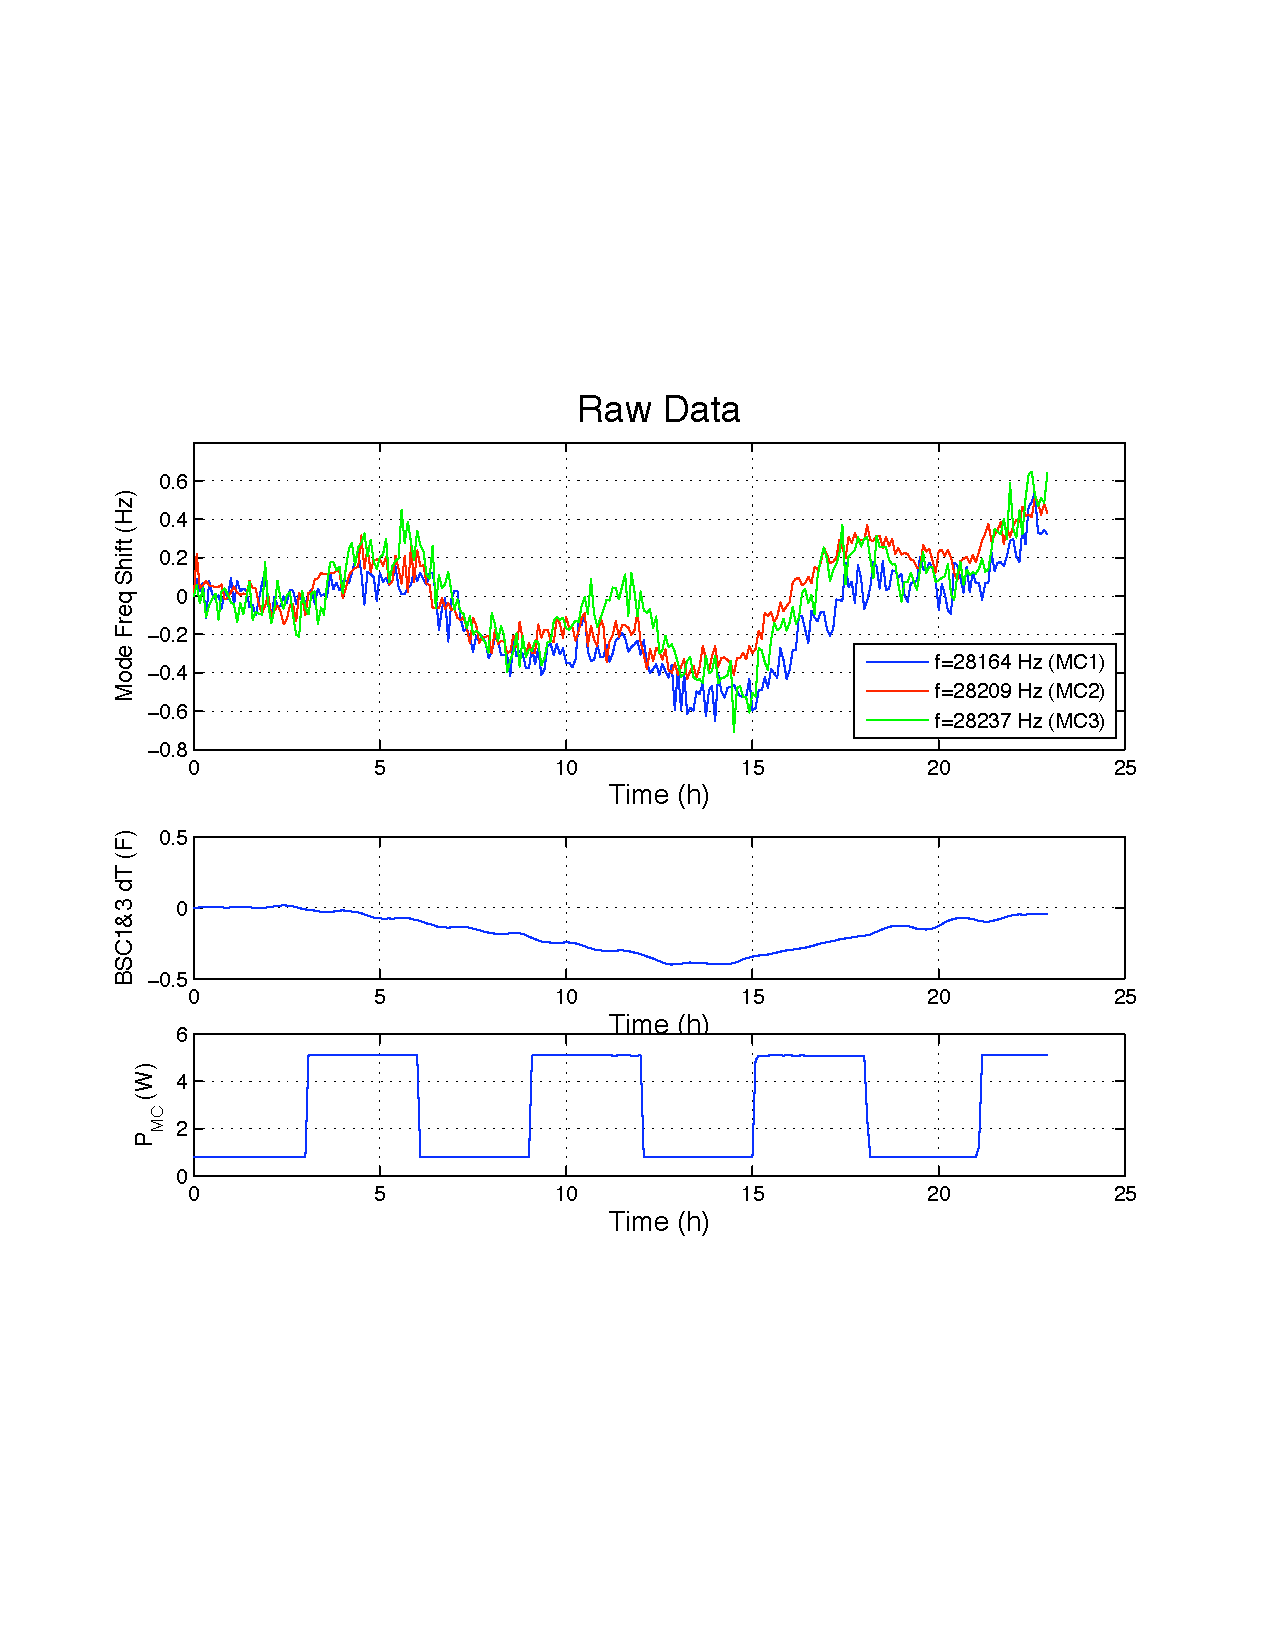
\includegraphics[width=1.0\columnwidth]{figures/MCdrumheadFeb08_raw.pdf}
%\includegraphics[width=1.0\columnwidth]{figures/MCabsorption_labelled.pdf}
\caption[Data from the mode cleaner absorption measurement]{Data from
  the mode cleaner absorption measurement. Power into the MC was
  cycled between 0.9~W and 5.1~W at 3 hour intervals (bottom frame)
  and the change in frequency of the drumhead mode of each mirror was
  recorded (top frame). The ambient temperature (middle frame) was
  also recorded in order to correct for its effects.}
%\textcolor{blue}{This is Valera's plot from Feb. 9, 2008}
\label{fig:MCabsorption}
\end{centering}
\end{figure}

\begin{table}
\centering
\caption[Absorption values for the Livingston and Hanford mode
 cleaner mirrors]{Absorption values for the Livingston and Hanford mode
 cleaner mirrors before (in parentheses) and after drag wiping. The precision is $\pm 10\%$.} 
%(from the March 8, 2008 elog and uses Muzammil's factor of $14/48$ correction.)
\begin{tabular}{l l l}
\hline
mirror & Livingston & Hanford\\
% mirror & before & after & before & after \\
% \hline\hline
% MC1 & 18.7 & 2.1  & 6.1  & 5.8 \\
% MC2 & 5.5  & 2.0  & 23.9 & 7.6 \\
% MC3 & 12.8 & 3.4  & 12.5 & 15.6 \\
\hline
MC1 & 2.1 ppm (18.7 ppm) & 5.8 (6.1 ppm) \\
MC2 & 2.0 ppm (5.5 ppm) & 7.6 (23.9 ppm) \\
MC3 & 3.4 ppm (12.8 ppm) & 15.6 (12.5 ppm) \\
\hline
\end{tabular}
\label{tab:MCabsorption2}
\end{table}


\subsubsection{Faraday isolator losses} 
The Faraday isolator was the second greatest source of power loss with
its transmission of 93\%. This was an improvement over the
86\% transmission of the Initial LIGO FI. The most lossy element in the
Faraday isolator was the thin film polarizer, accounting for 4\% of
total losses. The integrated losses from AR coatings and absorption in the
TGGs, CWPs, HWP, and DKDP account for the remaining 3\% of missing power. 


\subsection{Faraday Isolation Ratio}
The isolation ratio is defined as the ratio of power incident on the
Faraday in the reverse direction (the light reflected from the
interferometer) to the power transmitted in the 
reverse direction and is often quoted in decibels: isolation ratio~=~$10
\log_{10}(P_{in-reverse}/P_{out-reverse})$.  We measured the isolation ratio of the
Faraday isolator as a function of input power both in air prior to
installation and \emph{in situ} during Enhanced LIGO operation.

To measure the in-vacuum isolation ratio, we misaligned the
interferometer arms so that the input beam would be 
promptly reflected off of the $97\%$ reflective recycling mirror. This
also has the consequence that 
the Faraday isolator is subjected to twice the input
power. Our isolation monitor was a pick-off of the backwards 
transmitted beam taken immediately after transmission
through the Faraday that we sent out of a vacuum chamber
viewport. Refer to the \emph{isolation check beam} in 
Fig. \ref{fig:IOschematic}. The in air measurement was done similarly,
except in an optics lab with a reflecting mirror placed directly after
the Faraday. 

\begin{figure}
\begin{centering}
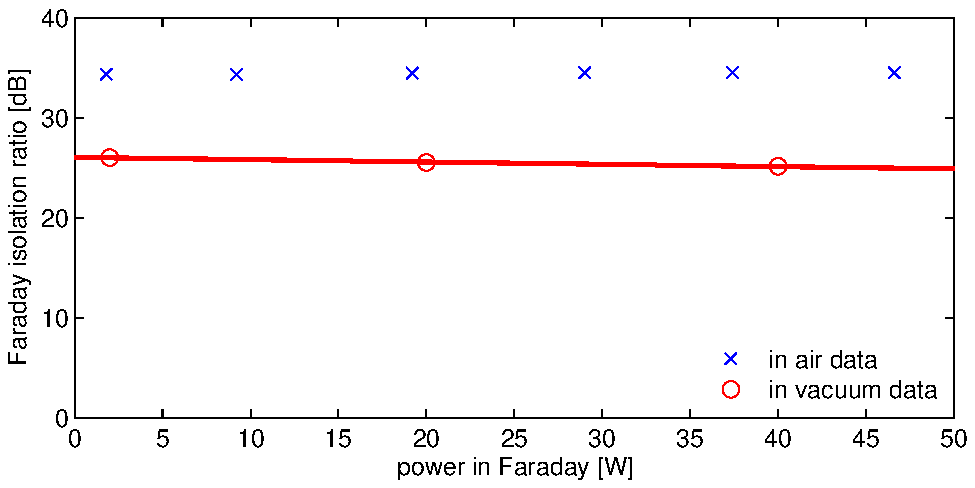
\includegraphics[width=1.0\columnwidth]{figures/FaradayIR.pdf}
\caption[Faraday isolator isolation ratio as measured in air and in
vacuum]{Faraday isolator isolation ratio as measured in air prior to
  installation and \emph{in situ} in vacuum. The isolation worsens by
  a factor of 6 upon placement of the Faraday in vacuum due to lack of
  air convection. The solid line is a linear fit to the in-vacuum
  data, indicating a degradation in isolation of 0.02 dB/W.}
\label{fig:IR}
\end{centering}
\end{figure}

Figure \ref{fig:IR} shows our isolation ratio data. Most notably, we
observe an isolation decrease of a factor of six upon placing the
Faraday isolator in vacuum, a result consistent with that reported by
Ref. \citep{TheVIRGOCollaboration2008Invacuum}. In air the isolation
ratio is a constant 34.46 $\pm$ 0.04 dB from low power up to 47~W, and
in vacuum the isolation ratio is 26.5 dB at low power. The underlying
cause is the absence of cooling by air convection. If we attribute the
loss to the TGGs, then based on the change in TGG polarization
rotation angle necessary to produce the measured isolation drop of
8~dB and the temperature dependence of the TGG's Verdet constant, we
can put an upper limit of 11~K on the crystal temperature rise from
air to vacuum. Furthermore, a degradation of 0.02~dB/W is measured in
vacuum.

\subsection{Thermal steering}
We measured the \emph{in situ} thermal angular drift of both the beam
transmitted through the mode cleaner and of the reflected beam from
the Faraday isolator with up to 25~W input power. Just as for the
isolation ratio measurement, we misaligned the interferometer arms so
that the input beam would be promptly reflected off of the recycling
mirror. The Faraday rotator was thus subjected to up to 50~W total
and the MC to 25~W. 

Pitch and yaw motion of the mode cleaner transmitted and
interferometer reflected beams were recorded using the quadrant
photodiode (QPD) on the Input Optics table and the RF alignment
detectors on the Interferometer Sensing and Control table (see
Fig. \ref{fig:IOschematic}). There are no lenses between the MC waist
and its measurement QPD, so only the path length between the two were
needed to calibrate in radians the pitch and yaw signals on the
QPD. The interferometer reflected beam, however, passes through
several lenses. Thus, ray transfer matrices and the two alignment
detectors were necessary to extract the Faraday drift calibration.

Figure \ref{fig:drift} shows the calibrated beam steering data. The
angle of the beam out of the mode cleaner does not change measurably
as a function of input power in yaw (4.7~nrad/W) and changes by only
440~nrad/W in pitch. For the Faraday isolator, we record a beam drift
originating at the center of the Faraday rotator of 1.8~\microrad/W in
yaw and 3.2~\microrad/W in pitch. Therefore, when ramping the input
power up to 30~W during a full interferometer lock, the upper limit on
the drift experienced by the reflected beam is about 100
\microrad. This is a thirty-fold reduction with respect to the Initial
LIGO Faraday isolator and represents a fifth of the beam's divergence
angle, $\theta_{div}$~=~490 \microrad.

\begin{figure}
\begin{centering}
% \includegraphics[width=1.0\columnwidth]{figures/MC_FI_drift_labelled.pdf}
\subfigure[Angular motion
  of the beam at the MC waist and FI rotator as the input power is
  stepped. The beam is double-passed through the Faraday isolator, so
  it experiences twice the input power.]{\includegraphics[width=1.0\columnwidth]{figures/forthesis_refldriftx10.pdf}}
\subfigure[Average beam angle per
  power level in the MC and FI. Linear fits to the data are also
  shown. The slopes for MC yaw, MC pitch, FI yaw, and FI pitch,
  respectively, are 0.0047, 0.44, 1.8, and 3.2 \microrad/W.]{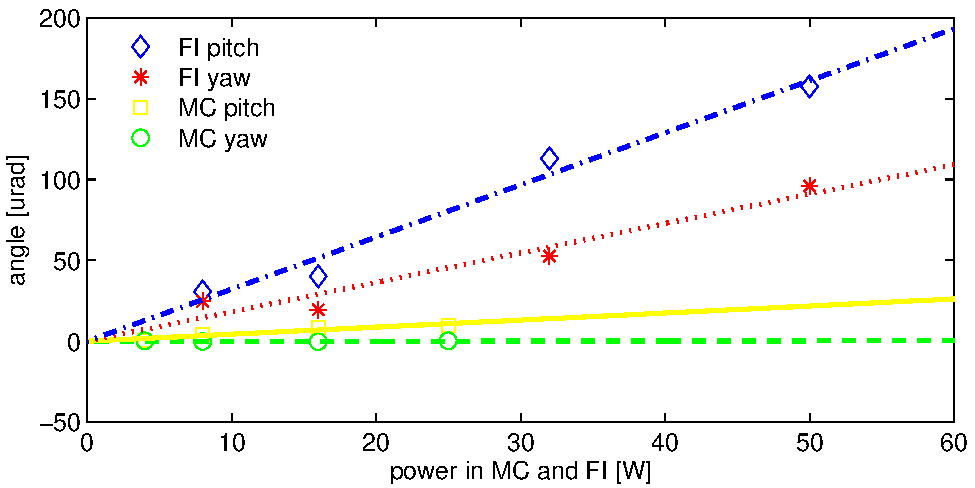
\includegraphics[width=1.0\columnwidth]{figures/alldrift.pdf}}
\caption[Mode cleaner and Faraday isolator thermal drift data.]{Mode
  cleaner and Faraday isolator thermal drift data.}
\label{fig:drift}
\end{centering}
\end{figure}


\subsection{Thermal Lensing}
We measured the profiles of both the beam transmitted through the
mode cleaner and the reflected beam picked off by the Faraday isolator
at low ($\sim$~1~W) and high ($\sim$~25~W) input powers to assess the
degree of thermal lensing induced in the MC and FI. Again, we
misaligned the interferometer arms so that the input beam would be
promptly reflected off the recycling mirror. We picked off a fraction
of the reflected beam on the Interferometer Sensing and Control table
and of the mode cleaner transmitted beam on the Input Optics table
(refer to Fig. \ref{fig:IOschematic}), placed lenses in each of their
paths, and measured the beam diameters at several locations on either
side of the waists created by the lenses. A change in the beam waist
size or position as a function of laser power indicates the presence
of a thermal lens.

\begin{figure}
\begin{centering}
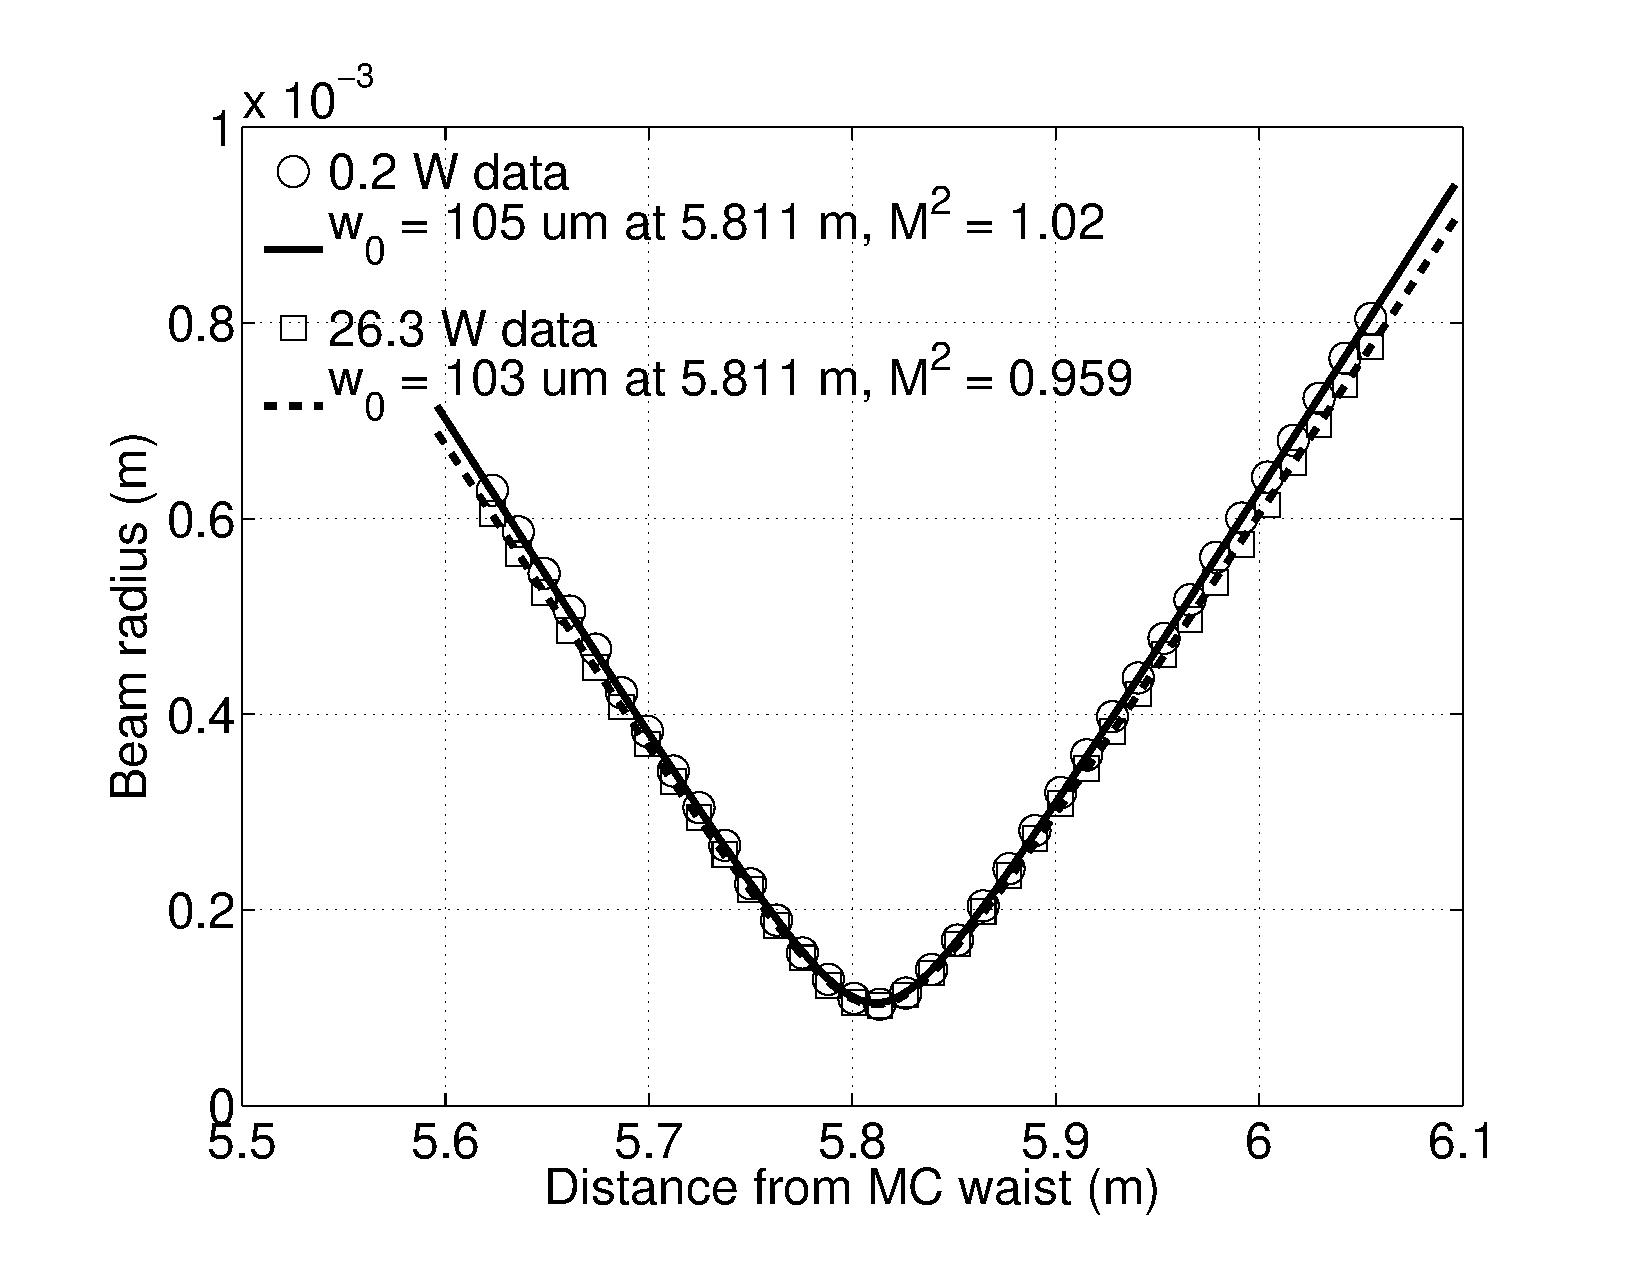
\includegraphics[width=1.0\columnwidth]{figures/MCTrans_datafit.pdf}
\caption[Profile at high and low powers of mode cleaner transmitted
beam]{Profile at high and low powers of a pick-off of the beam
  transmitted through the mode cleaner. The precision of the beam
  profiler is $\pm 5\%$. Within the error of the measurement, there
  are no obvious degradations.}
\label{fig:MC_lensing}
\end{centering}
\end{figure}

\begin{figure}
\begin{centering}
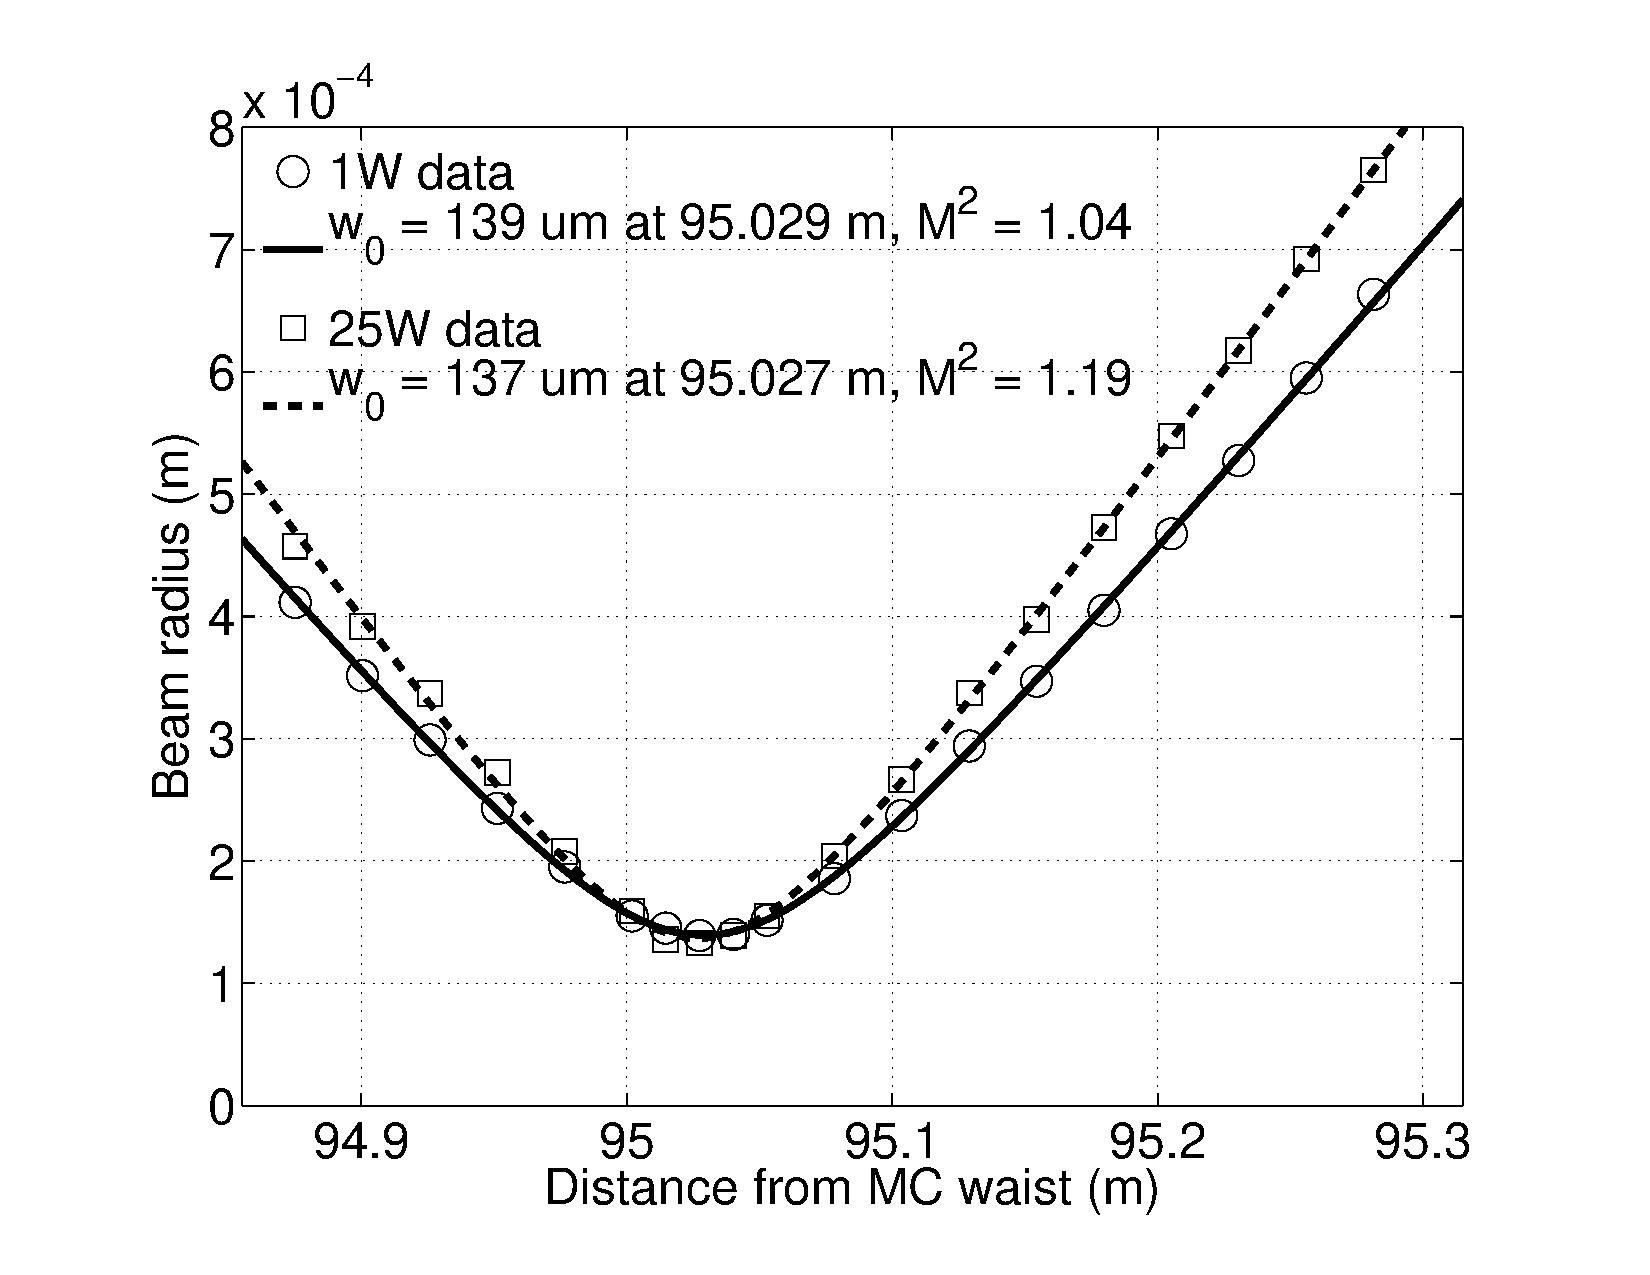
\includegraphics[width=1.0\columnwidth]{figures/REFL_datafit.pdf}
\caption[Faraday isolator thermal lensing data]{Faraday isolator
  thermal lensing data. With 25 W into the Faraday isolator
  (corresponding to 50 W in double pass), the beam has a steeper
  divergence than a pure TEM$_{00}$ beam, indicating the presence of
  higher order modes. Errors are $\pm 5.0\%$ for each data point.}
\label{fig:FI_lensing}
\end{centering}
\end{figure}

As seen in Fig. \ref{fig:MC_lensing} and \ref{fig:FI_lensing}, the
waists of the two sets of data are collocated--no thermal lens is
measured. For the Faraday isolator, the divergence of the low and high
power beams differs, indicating that the beam quality degrades with
power. The $M^2$ factor at 1~W is 1.04 indicating the beam is 
nearly perfectly a TEM$_{00}$ mode. At 25~W, $M^2$ increases to 1.19,
corresponding to increased higher order mode content. The percentage
of power in higher order modes depends strongly on the mode order and
relative phases of the modes, and thus cannot be determined from this
measurement \citep{Kwee2007Laser}.

The results for the mode cleaner data are consistent with no thermal
lensing. The high and low power beam profiles are within each
other's error bars and well below our requirements. 

We also measured the thermal lensing of the electro-optic modulator
prior to its installation in Enhanced LIGO by comparing beam profiles
of a 160~W beam with and without the EOM in its path. The data for
both cross-sections of the beam is presented in
Fig.~\ref{fig:EOMlensing}. We observe no significant thermal lensing
in the y-direction and a small effect in the x-direction. An upper
limit for the thermal lens in the x-direction can be calculated to be
greater than 4~m, which is 10 times larger than the Rayleigh range of
the spatial mode. The mode matching degradation is therefore less
than 1\%. Although a direct test for Advanced LIGO because of the
power used, this measurement also serves to demonstrate the
effectiveness of the EOM design for Enhanced LIGO powers.

\begin{figure}
\begin{centering}
%\includegraphics[width=1.0\columnwidth]{figures/Picture1.png}
\caption{EOM thermal lensing data.}
\label{fig:EOMlensing}
\end{centering}
\end{figure}


\subsection{Mode Matching}
We measured the effectiveness of the mode-matching telescope by taking
the ratio of power at the reflected port when all of the
interferometer cavities are on resonance to the power in the reflected
beam when the cavities are unlocked. Since the impedance matching is
near perfect, all light at the reflected port during interferometer
lock is attributable to a mode mismatch.  Initially, anywhere between
10\% and 17\% of the light was rejected by the cavity due to poor,
power-dependent mode matching.  After translating the mode-matching
telescope mirrors during a vacuum chamber incursion and upgrading the
other IO components, the ratio we measured was 8\% independent of
input power. The MMT succeeds at coupling 92\% of the light into the
interferometer at all times, marking both an improvement in MMT mirror
placement and success in eliminating measurable thermal issues.


\section{Implications for Advanced LIGO}
\label{sec:aLIGO}
As with other Advanced LIGO interferometer components, Enhanced LIGO
served as a technology demonstrator for the Advanced LIGO Input
Optics, albeit at lower laser powers The performance of the Enhanced
LIGO Input Optics components, at 20~W of input power allows us to
infer their performance in Advanced LIGO.  The requirements for the
Advanced LIGO Input Optics demand are for similar performance to
Enhanced LIGO, but with almost 8 times the laser power.

%EOM 
The Enhanced LIGO electro-optic modulator showed no thermal lensing,
degraded transmission, nor damage in over 1 million hours of sustained
operation. Measurements of the thermal lensing in RTP at powers up to
160 W show a relative power loss of $< 0.4\%$, indicating that thermal
lensing should be negligible in Advanced LIGO.  Peak irradiances in
the EOM will be approximately four times that of Enhanced LIGO (a 45\%
larger beam diameter will somewhat offset the increased power).
Testing of RTP at 10 times the expected Advanced LIGO irradiance over
100~hours show no signs of damage or degraded transmission.

The mode cleaner showed no measurable change in operational state as a
function of input power.  This bodes well for the Advanced LIGO mode
cleaner.  Compared with the Enhanced LIGO mode cleaner, the Advanced
LIGO mode cleaner is designed with a lower finesse (520) than Initial
LIGO (1282).  For 150~W input power, the Advanced LIGO mode cleaner
will operate with 3 times greater stored power than Initial LIGO.  The
corresponding peak irradiance is 400~kW/m$^2$, well below the
continuous wave coating damage threshold.  Absorption in the Advanced
LIGO mode cleaner mirror optical coatings has been measured at
0.5~ppm, roughly four times less than the best mirror coating
absorption in Enhanced LIGO, so the expected thermal loading due to
coating absorption should be reduced in Advanced LIGO.  The larger
Advanced LIGO mode cleaner mirror substrates and higher input powers
result in a significantly higher contribution to bulk absorption,
roughly 20 times Enhanced LIGO, however the expected thermal lensing
leads to small change ($< 0.5 \%$) in the output mode
\citep{Arain2007Note}.

The Enhanced LIGO data obtained from the Faraday isolator allows us to
make several predictions about how it will perform in Advanced LIGO.
The measured isolation ratio decrease of 0.02~dB/W will result in a
loss of 3~dB for a 150~W power level expected for Advanced LIGO
relative to its cold state.  However, the Advanced LIGO Faraday
isolator will employ an adjustable half wave plate \emph{in situ},
which will allow for a partial restoration of the isolation ratio. The
maximum thermally induced angular steering expected is 480 \microrad
(using a drift rate of 3.2 \microrad/W), approximately equal to the
beam divergence angle. This has some implications for the Advanced
LIGO length and alignment sensing and control system, since the
reflected Faraday isolator beam is used as a sensing beam. Operation
of Advanced LIGO at high powers will likely require the use of a beam
stabilization servo to lock the position of the reflected beam on the
sensing photodiodes.  Although no measurable thermal lensing was
observed (no change in the beam waist size or position), the measured
presence of higher order modes in the FI at high powers is suggestive
of imperfect thermal lens compensation by the DKDP.  This potentially
can be reduced by a careful selection of the thickness of the DKDP to
better match the absorbed power in the TGG crystals.

\section{Summary}
\label{sec:summary}
In summary, we have presented a comprehensive investigation of the
Enhanced LIGO Input Optics, including the function, design, and
performance of the IO.  Several improvements to the design and
implementation of the Enhanced LIGO IO over the Initial LIGO IO have
lead to improved optical throughput and coupling to the main
interferometer through a substantial reduction in thermo-optical
effects in the major IO optical components, including the
electro-optic modulators, mode cleaner, and Faraday isolator.  The IO
performance in Enhanced LIGO enables us to infer its performance in
Advanced LIGO, and indicates that high power interferometry will be
possible without severe thermal effects.


% \section{Radiation pressure in MC}
% \textcolor{blue}{Maybe write up April 4, 2009 notebook derivation of
%   radiation pressure length spring in MC. Also, Rana has a noise
%   budget elog entry April 3, 2009.}

\chapter{The Angular Motion of the Interferometer}

% normalize out seismic motion for wfs on / wfs off residual motion comparison

% include shot noise on at least WFS1 sensor noisebudget; maybe limiting
% depending on power used

% how low can you go before it falls apart? valera and kate tried this
% out--find in elog


% RF offsets changing 

% possible in test runs to inc. hard/soft modes to 3
% hz, higher than ever before; but operationally, need lower. talk to
% matt and lisa to make sure to handle things politically correctly.

% calculate time-lag as cavity light responds to mirror displacements --> damping from RP


For light to resonate in the interferometer, the mirrors need to point at one another and remain stationary with respect to this pointing. In practice, however, the mirrors are subject to external disturbances. 
%move around due to three torques inputs to each mirror: the suspension, the actuators, and radiation pressure. 
Each torque produces an angular displacement of the mirror as governed by the mirror's torque to angle transfer function and results in either a static or dynamic misalignment.

The dynamic misalignments arise from torque introduced through the suspension from ground motion and through the actuators from an unbalanced piston force. Both of these torques create an angular motion independent of the state of the mirror's pointing. Radiation pressure torque, however, stands apart; its effect depends on the pointing of the mirror. A consequence is that even when all of the mirrors are perfectly aligned at all frequencies, the simple existence of light in the interferometer makes the arm cavities statically unstable when high enough laser powers are used.

This chapter discusses the causes of mirror angular displacement and the effects of residual mirror motion on the interferometer. Background material is provided as necessary, such as the dynamics of torsion pendula, and the geometric eigenfunctions of linear cavities. The need for an Angular Sensing and Control subsystem will be apparent.




\section{Sources of angular mirror motion}
There is a continuous stream of changing torque inputs to the mirrors that cause them to twist and turn in pitch and in yaw. Some torque inputs exist regardless of the state of the interferometer, while others are a direct consequence of the control systems. The primary torque inputs are introduced here, and further discussion of some of them is found later in the chapter. The list includes:
\begin{itemize}
\item ground motion \vspace{-10pt} 
\item seismic isolation \vspace{-10pt} 
\item coil actuators (length to angle) \vspace{-10pt}
%\item thermal noise of pitch and yaw modes? \vspace{-10pt}
\item radiation pressure \vspace{-10pt}
\item noise impression from the angular control system 
\end{itemize}




\subsection{Ground motion} 
The most egregious of these torque inputs is ground motion that makes its way through the multiple stages of seismic isolation to the mirror suspensions. 
This is the only source of angular motion that is present regardless of the state of interferometer operation. An example of the shape and amount of angular motion experienced by the core optics due to seismic noise during a relatively quiet seismic time is shown in Fig. \ref{fig:seismicMirror}. These spectra include the effect of local velocity damping since the optical levers are always on (see Sec. \ref{sec:suspension}). The rms mirror motion is of the order $10^{-7}$ rad. This is the motion that needs to be controlled interferometrically.

\begin{figure}
\begin{centering}
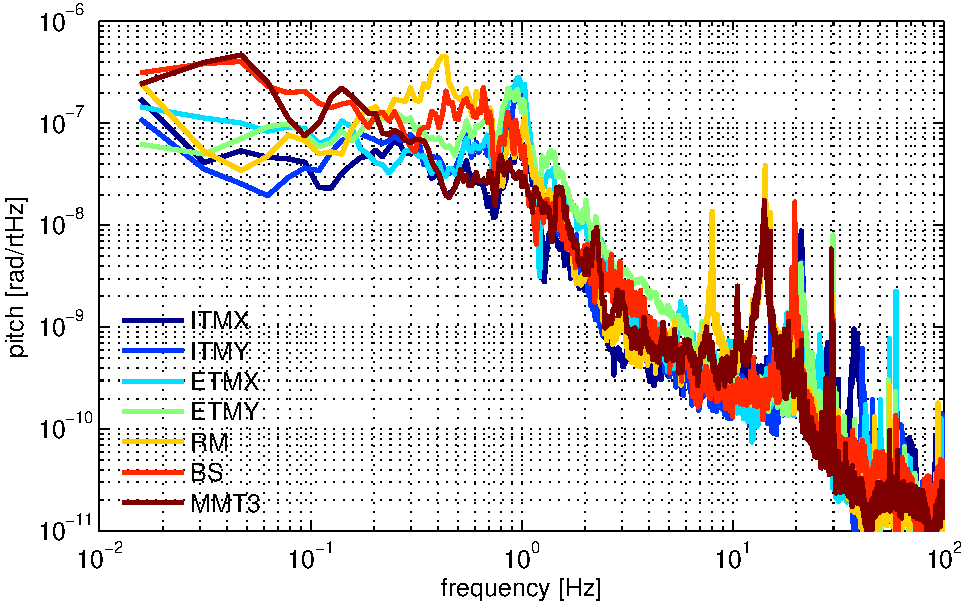
\includegraphics[width=1.0\columnwidth]{figures/seismic_mirrormotion.pdf}
%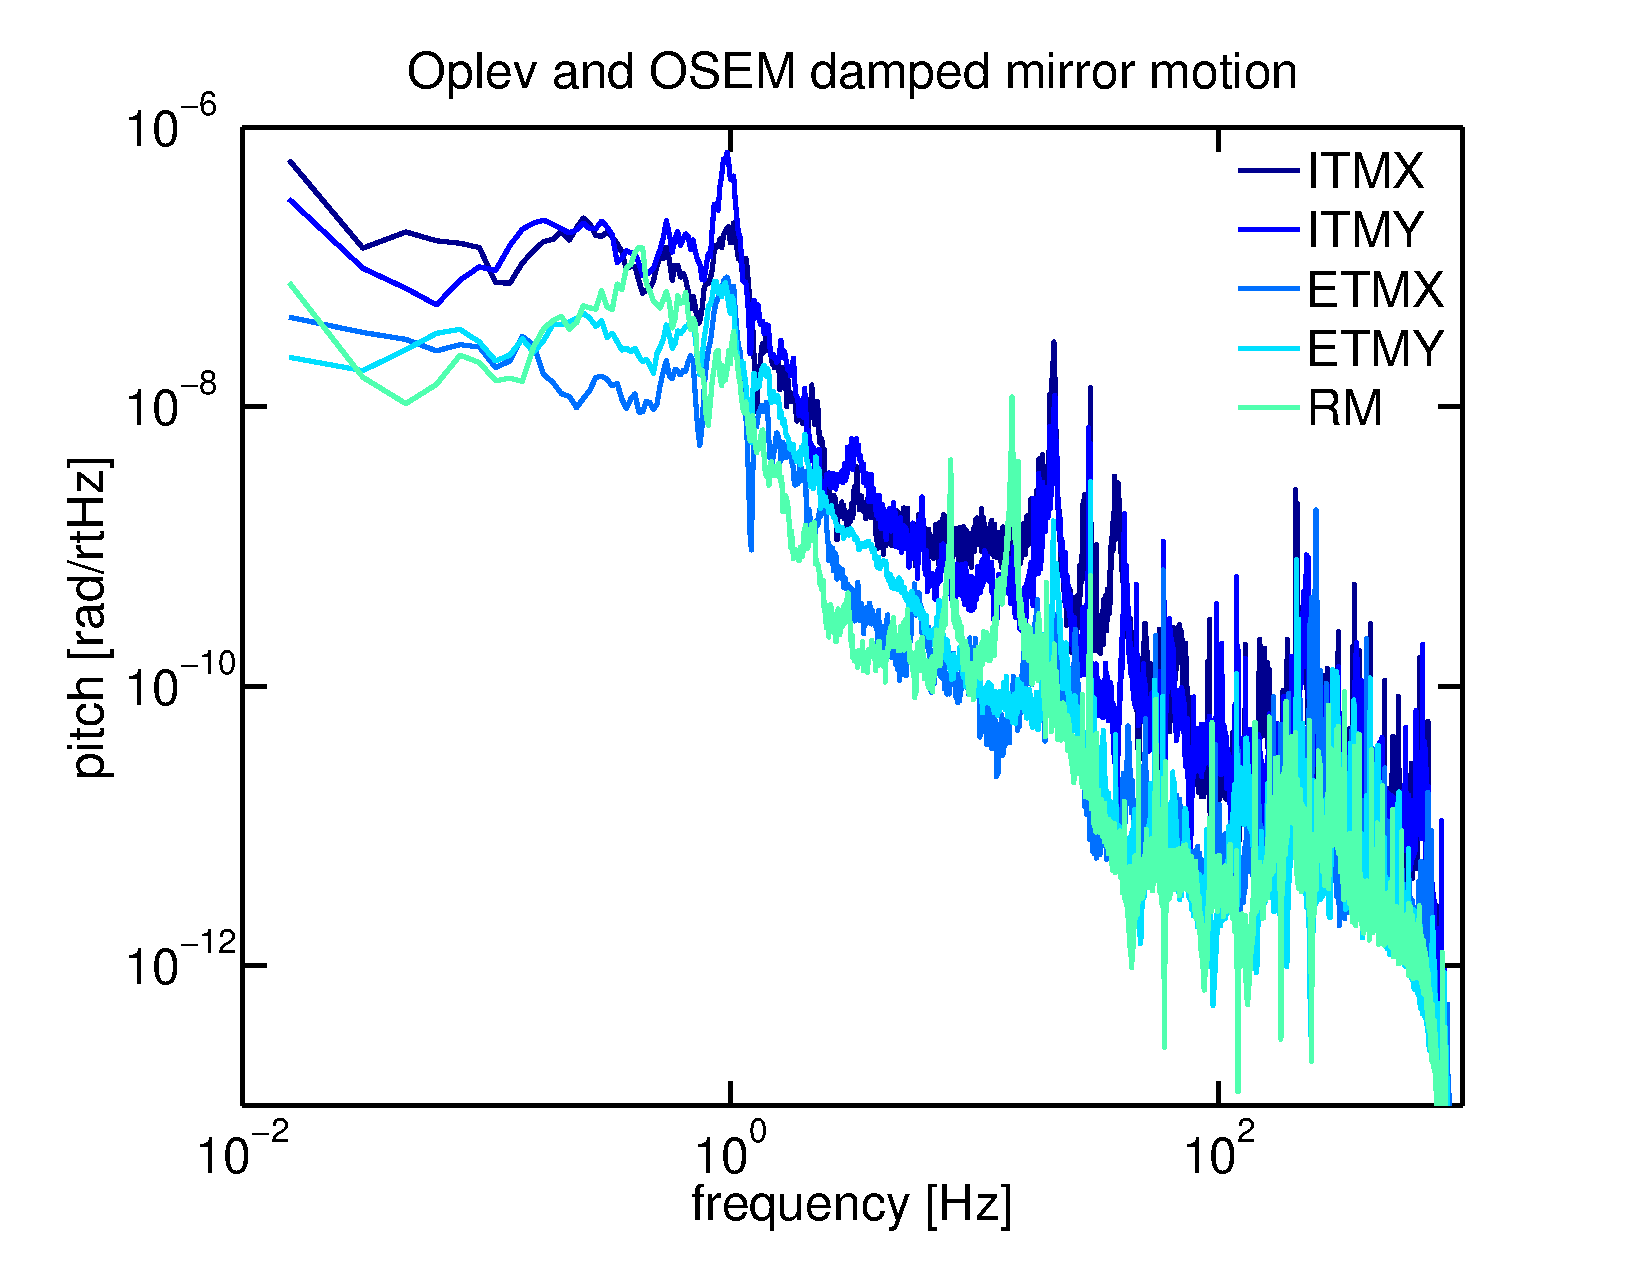
\includegraphics[width=0.7\columnwidth]{figures/ifodark_mirrormotion.pdf}
\caption[Typical angular motion of the core suspended mirrors in the
  absence of interferometric control]{Typical angular motion of the core suspended mirrors in the
  absence of interferometric control. Velocity damping provided by the
 OSEMs and the optical levers is present. Once the interferometer is locked, the OSEM damping is ramped off. 
  % Above about 30 Hz, the plot
  % does not represent real motion; the spectrum is limited by sensor
  % (optical lever) noise.
}
\label{fig:seismicMirror}
\end{centering}
\end{figure}

% Take a model of the optical lever open loop gains and a spectrum of
% optical lever error signal at a time when the interferometer is
% unlocked, but optical levers are on to calculate the background mirror
% motion due to seismic noise. Show the effect at a select few different
% times of day, probably for just one mirror. Write this section once I
% see what I have to present.

Proof that this motion indeed originates from the ground can be provided by computing Wiener filters for the seismomter signals to see their coherence with the optical lever error signals. Figures are in appendix \ref{sec:oplev_contributions}





\subsubsection{Seismic isolation}
Although the multiple layers of seismic isolation serve to make interferometer operation possible \textcolor{blue}{write something better!}, minor imperfections in their implementation can result in them serving as coupling mechanisms to mirror angle. The path from ground to mirror can be broken into two distinct parts: HEPI + stack position to angle, and suspension position to angle. The seismic tables (HEPI at LLO) are actively actuated upon in position, ie. for the tidal servo. Any position to angle coupling will twist the table. The suspension 


\subsubsection{Seismometers}
The seismometers are sensitive to six degrees of freedom: x, y, z, and rotation about x, y, and z. Ideally, they are set up to only measure ground motion in x, y, and z, but the signals may be contaminated by some tilt as well. \textcolor{blue}{???}




\subsection{Coil actuators} 
\label{sec:L2A}
The imperfect piston drive of the actuators on the rear of the test masses due to length control is another torque input, albeit inconsequential. The length of the cavities is carefully controlled (that's what we strive to be most sensitive to!) and any imbalances between the four electromagnets on a single mirror will create a coupling from length drive to angle (L2A). This effect is measurable, but is carefully tuned out through selecting appropriate digital gains for each of the coils. Typically, the gain variation from unity is up to 10\%. The residual is about 1\%. For the typical rms length drive of 1~\micron on a core optic and osems separated by a distance of $\sqrt{2} R$ where $R$ is the radius of the optic, the 1\% L2A coupling results in a $10^{-8}$ radian displacement:
\begin{equation}
\theta = \frac{0.01 * 10^{-6} \mbox{ m}}{\sqrt{2} * 0.125 \mbox{ m}} \approx 10^{-8} \mbox{ rad}.
\end{equation}

% Maybe include a figure that takes a typical length control spectrum signal to an optic and multiply by the above factors to show spectrum of angular motion induced by 1\% L2A.



\subsection{Radiation pressure} 
Radiation pressure creates a torque when the beam impinges the mirror
off-center. The force on the mirror due to radiation pressure is
derived from the change in momentum of a photon upon reflection off
the mirror and results in:
\begin{equation}
F_{rp} = \frac{2 P} {c}
\end{equation}
where $P$ is the power of the light reflected by the mirror and $c$ is the
speed of light. Assuming the beam of photons strikes the mirror
perpendicular to its surface, the torque exerted on a mirror due to
radiation pressure is
\begin{equation}
\tau_{rp} = \frac{2 P x} {c}
\label{eq:tau_rp}
\end{equation}
where $x$ is the distance of the beam from the mirror's center of mass. For a 40~kW beam 1~mm off-center, the torque is on the order of $10^{-7}$ Nm, corresponding to an angular displacement of the order $10^{-7}$ rad as determined by the pendulum torque to angle transfer function (see \ref{sec:pendTF}).

Amongst the various torque inputs, radiation pressure plays a unique role in mirror motion because the torque it exerts depends on the angles of the mirrors. 
%This is a result of the geometric coupling between beam displacements and mirror angles as will be shown in the next chapter. Radiation pressure therefore acts as an angular spring. 
It is best treated not as an external torque, but as a modification to the pendulum torque to angle transfer function. Part of the next chapter dedicates a discussion to this matter. In all, radiation pressure shapes the angular dynamics of the mirrors in LIGO and plays an important role in the design of an angular control system.



\subsection{Noise from angular control}
The angular control system, which strives to counteract the above torque inputs to reduce angular motion, introduces angular mirror motion itself. The primary way it contributes noise is through imperfect sensing of the angular displacements. The alignment is also undercontrolled, which ends up allowing the control system to impress input beam motion on the mirrors. These issues and others are explained in more detail in \ref{sec:ASClimits}.



\section{Tolerance for angular motion}
% Unlike DARM where the uncontrolled length displacement is what matters, it's the controlled  motion of the mirrors that matters for angular displacement. Too much residual motion, and both the lever arm effect and power fluctuations create noise in DARM. To prevent angular mirror motion from creating length displacements, the mirrors must not move more than $10^{-8}$ rad rms and the beam spots no more than 1 mm rms, as The residula motion must be held below 

The requirements for how much motion is tolerable stem from two effects of misalignment that directly couple to strain sensitivity: power build-up degradation, and angle to length coupling. The misalignment tolerances are dictated by what is necessary to prevent the strain sensitivity of the perfectly aligned interferometer from degrading by more than 0.5\% in the detection band of 40-7000~Hz \cite{Fritschel1997Alignment}.

Since the strain sensitivity is proportional to the power buildup (see Eq. \ref{}), a decrease in circulating power directly results in a decrease of shot-noise-limited DARM. Differing power fluctuations in the two arm cavities results in a changing contrast defect, a difference in the amount of light returning from one arm compared to the other, which increases the shot noise at the AS port. Too large of power fluctuations in the power recycling cavity makes for inconsistent signal to noise ratios for the signals that depend on sideband power. To maintain a power buildup within 1\% of maximum, the core optics must have an angular displacement of less than $10^{-8}$ rad rms with respect to the cavity axis \cite{ISCGroup1998ASC}. The derivation of power buildup as a function of mirror angle displacement is found in Appendix \ref{sec:cavitypower}.


\textcolor{blue}{work this paragraph in somewhere}
The idea is that when the axis of rotation of a mirror coincides with the center of the beam, any tilt of the mirror about this axis does not affect the path length of the reflected beam. However, if there is a mismatch between rotation axis and beam location, then the light will pick up a longitudinal phase shift when the mirror is tilted. During a full interferometer lock, this is recorded by DARM.



When the beam is located a distance $x$ away from the center of the mirror, an
angular displacement of the mirror $\theta$ about its center results in a path
length change of the beam
\begin{equation}
\Delta{L} = x * \theta
\end{equation}
which has a direct impact on DARM. Therefore, the alignment specifications must include not only tolerable levels of angular motion, but requirements for the physical centering of the beam spots on the mirrors. As detailed in Ref. \cite{ISCGroup1998ASC}, the beams must be centered on the core optics within 1~mm. At DC, for x ~=~1 mm and $\theta = 10^{-7}$ rad, $\Delta{L} = 10^{-10}$ m which is four orders of magnitude below the DARM rms of $10^{-6}$ m. \textcolor{blue}{Convolve my bsm spectra and residual mirror motion spectra to show example.}




\section{Overview of interferometer alignment}
\label{sec:alignment_overview}

There are 8 mirrors whose pitch and yaw angles must be sensed and controlled. The sensing is accomplished by 8 sensors, which fall into three groups:
\begin{itemize}
\item camera image (BS)  \vspace{-10pt}
\item quadrant photodiodes (QPDX, QPDY) \vspace{-10pt}
\item wavefront sensors (WFS1, WFS2, WFS3, WFS4)
\end{itemize}
The alignment of these mirrors using these sensors can be simplified by considering the interferometer alignment as happening in two basic units: the input beam and the power recycled Fabry-Perot Michelson. The alignment of the latter is nearly self-contained and can in fact be compacted down to a representative single mirror. The remaining jobs are to align the input beam and this ``single mirror'' to one another and to keep the y-arm perpendicular to the x-arm.

The self-contained alignment of the power recycled Fabry-Perot Michelson is realized through the set of wavefront sensors (WFS), whose principle of operation is described in Section \ref{sec:wfs}. The pitch and yaw motions of the five mirrors in this unit, ETMX, ETMY, ITMX, ITMY, and the PRM, are sensed by the pitch and yaw of five WFS signals, WFS1Q, WFS2I, WFS2Q, WFS3I, and WFS4I, where I and Q denote in-phase and quadrature demodulation, respectively. These WFS look at light at the AS port, at the reflected port, and in the power recycling cavity. They control the relative motions of these five mirrors up to a couple Hz. 

The MMT-directed input beam and the interferometer ``mirror'' need to be aligned so that the input beam is perfectly reflected upon itself. The input beam follows the interferometer on about minute time scales, and at higher frequencies the interferometer follows the input beam. The low frequency matching of the input beam pointing to the interferometer ``mirror'' is realized through the pitch and yaw signals of QPDX, a QPD which monitors the position of the light transmitted through the x-arm, and the pitch and yaw signals of a camera that monitors the beam location on the beam splitter. These two alignment sensors adjust the pointing of MMT1 and MMT3 on about minute time scales. An example of the BS camera image is shown in Fig. \ref{fig:BCS}. The higher frequency matching of the input beam pointing to the interferometer is achieved by the reflected port Fabry-Perot Michelson wavefront sensors, up to a couple Hz.

\begin{figure} 
\begin{centering} 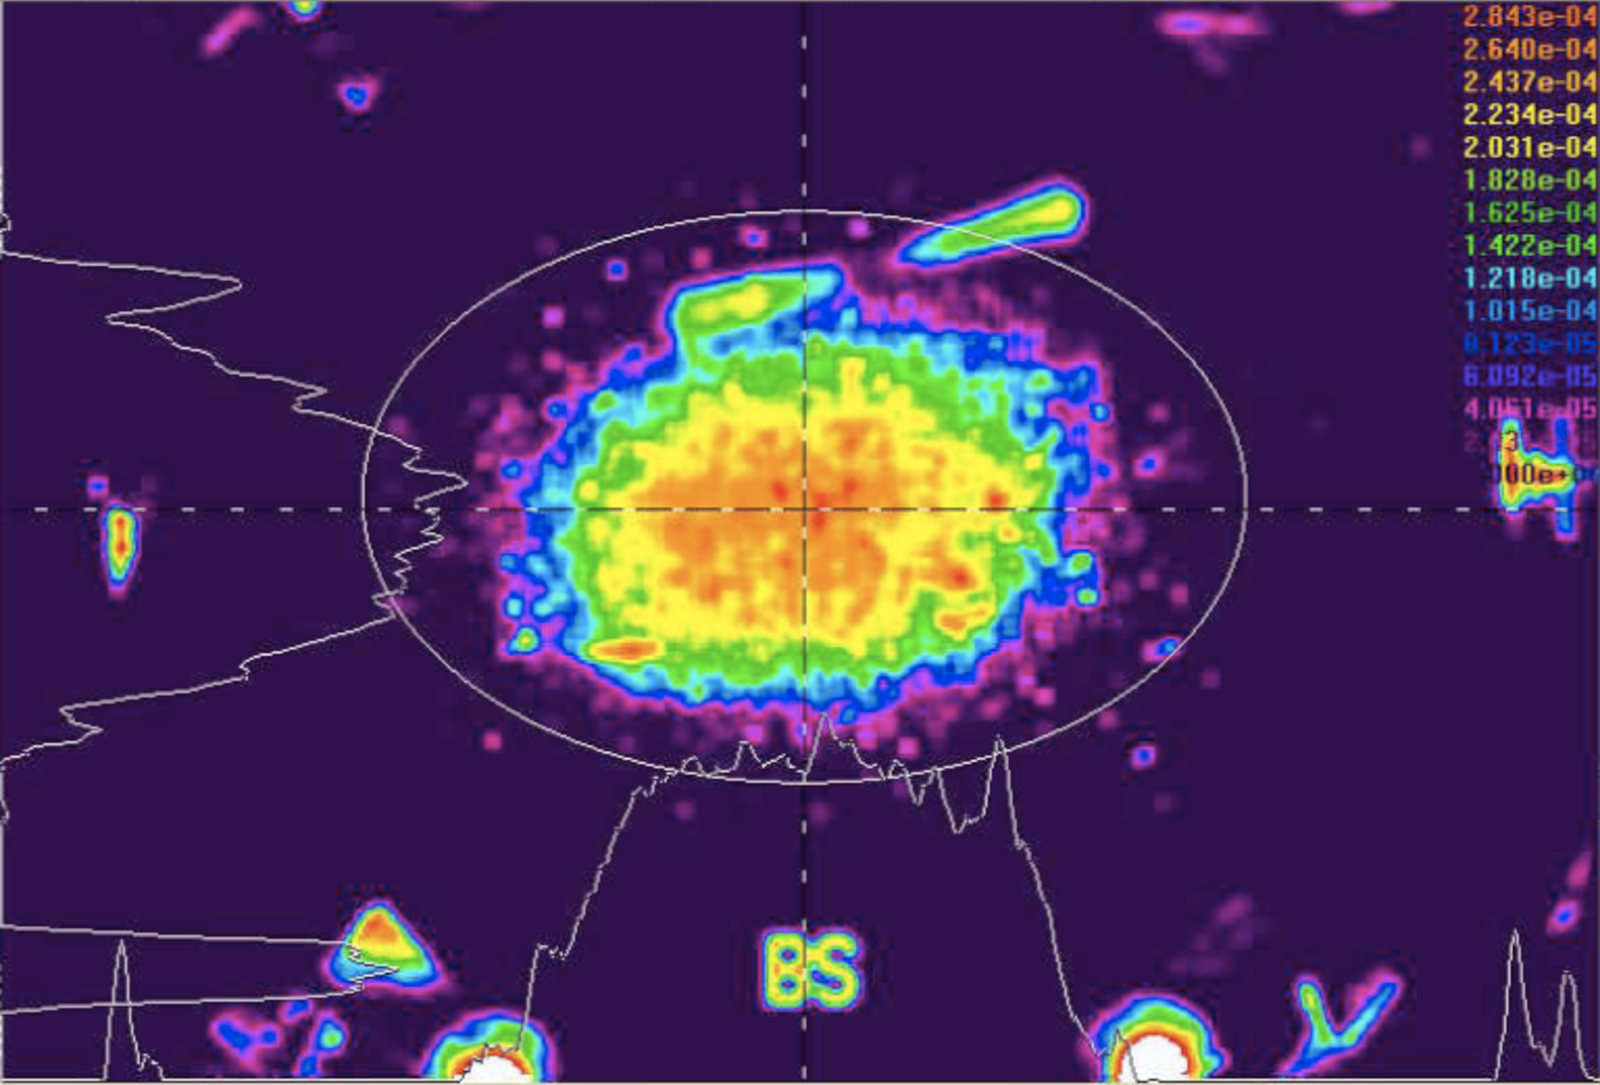
\includegraphics[width=0.6\textwidth]{figures/BCSspiricon.pdf} 
\caption[Beam centering servo image of beam splitter]{Image of beam on beam splitter as used in the beam centering servo. The beam appears stretched because the camera's viewing angle is at $45^{\circ}$ with respect to the mirror surface. The color scale is arbitrary.}
\label{fig:BCS}
\end{centering}
\end{figure}

The one additional step needed for full interferometer alignment is to maintain the orthogonality of the y-arm to the x-arm as the x-arm and input beam together move around. This is accomplished through the pitch and yaw signals of QPDY, the QPD that monitors the light transmitted through the y-arm, which sense how the beam splitter should be pointed. \footnote{QPDX also sends a signal to the BS to compensate for whatever it has MMT3 do.}

All mirror angles are of course interdependent and they must track each other. However, a rough hierarchy of who follows who can be established since ultimately the interferometer is bolted to the ground and necessarily maintains some DC orientation. This orientation comes from QPDX and QPDY, which are physically attached to piers standing on the ground and force the beams transmitted through the ETMs to stay put at a certain location on their sensors. In all, the input beam must make it to those two exact places and the other mirrors are left to line themselves up accordingly. A diagram of this alignment scheme is in Fig. \ref{fig:ASClayout}.

%two input beams, one to the x-arm, one to the y-arm; and the FPM

\begin{figure} \begin{centering} \includegraphics[width=0.8\textwidth]{figures/ASClayout_wctrl.pdf} 
\caption[Schematic of the alignment sensing and control system]{Schematic of the alignment sensing and control system, showing the placement of sensors and which mirrors they control. The QPD servo and Beam Centering Servo (BCS) together direct the input beam to follow the FPM unit on minute time scales. The QPD servo additionally keeps the BS properly directing light into the y-arm. The wavefront sensing servo maintains the alignment of the FPM mirrors with respect to each other up to several Hz. Each of the seven large optics has its own velocity damping optical lever servo.}
\label{fig:ASClayout}
\end{centering}
\end{figure}

This alignment process involving the WFS, QPDs, and BS camera relies on the entire interferometer already being locked. It manages the continuous fine-tuning of mirror angles so that maximal power buildup in the interferometer is maintained, and so that the interferometer does not wander from its linear operating point. How to achieve the initial alignment of all of the mirrors is an interesting process in itself and is documented in Appendix \ref{sec:initial_alignment}.




\section{Angular control limitations}
\label{sec:ASClimits}
The limits for how good we can do in controlling the angular motion of the interferometer are governed by how well we are able to sense the angular motion. Several of the wavefront sensors' signals are dark-noise-limited above 20-25~Hz, as seen in Fig. \ref{fig:WFSdarknoise}. And depending on the power level, WFS1Q may instead be limited by shot noise (see Eq. \ref{eq:shotnoise}). Any control signal derived from frequencies in the sensing noise limited regime will impress the sensor noise on the mirrors. This cannot be avoided entirely in the presence of feedback, but can be mitigated by including amongst the control filters a steep cut-off beginning at the sensor noise frequencies. 
%Ultimately, it is the WFS noise floor that determines the best possible achievable suppression. 

\begin{figure} \begin{centering} \subfigure{\includegraphics[width=0.333\textwidth]{figures/wfs1q_darkres.pdf}}\subfigure{\includegraphics[width=0.333\textwidth]{figures/wfs2i_darkres.pdf}}\subfigure{\includegraphics[width=0.333\textwidth]{figures/wfs2q_darkres.pdf}} 
\subfigure{\includegraphics[width=0.333\textwidth]{figures/wfs3i_darkres.pdf}}\subfigure{\includegraphics[width=0.333\textwidth]{figures/wfs4i_darkres.pdf}} 
%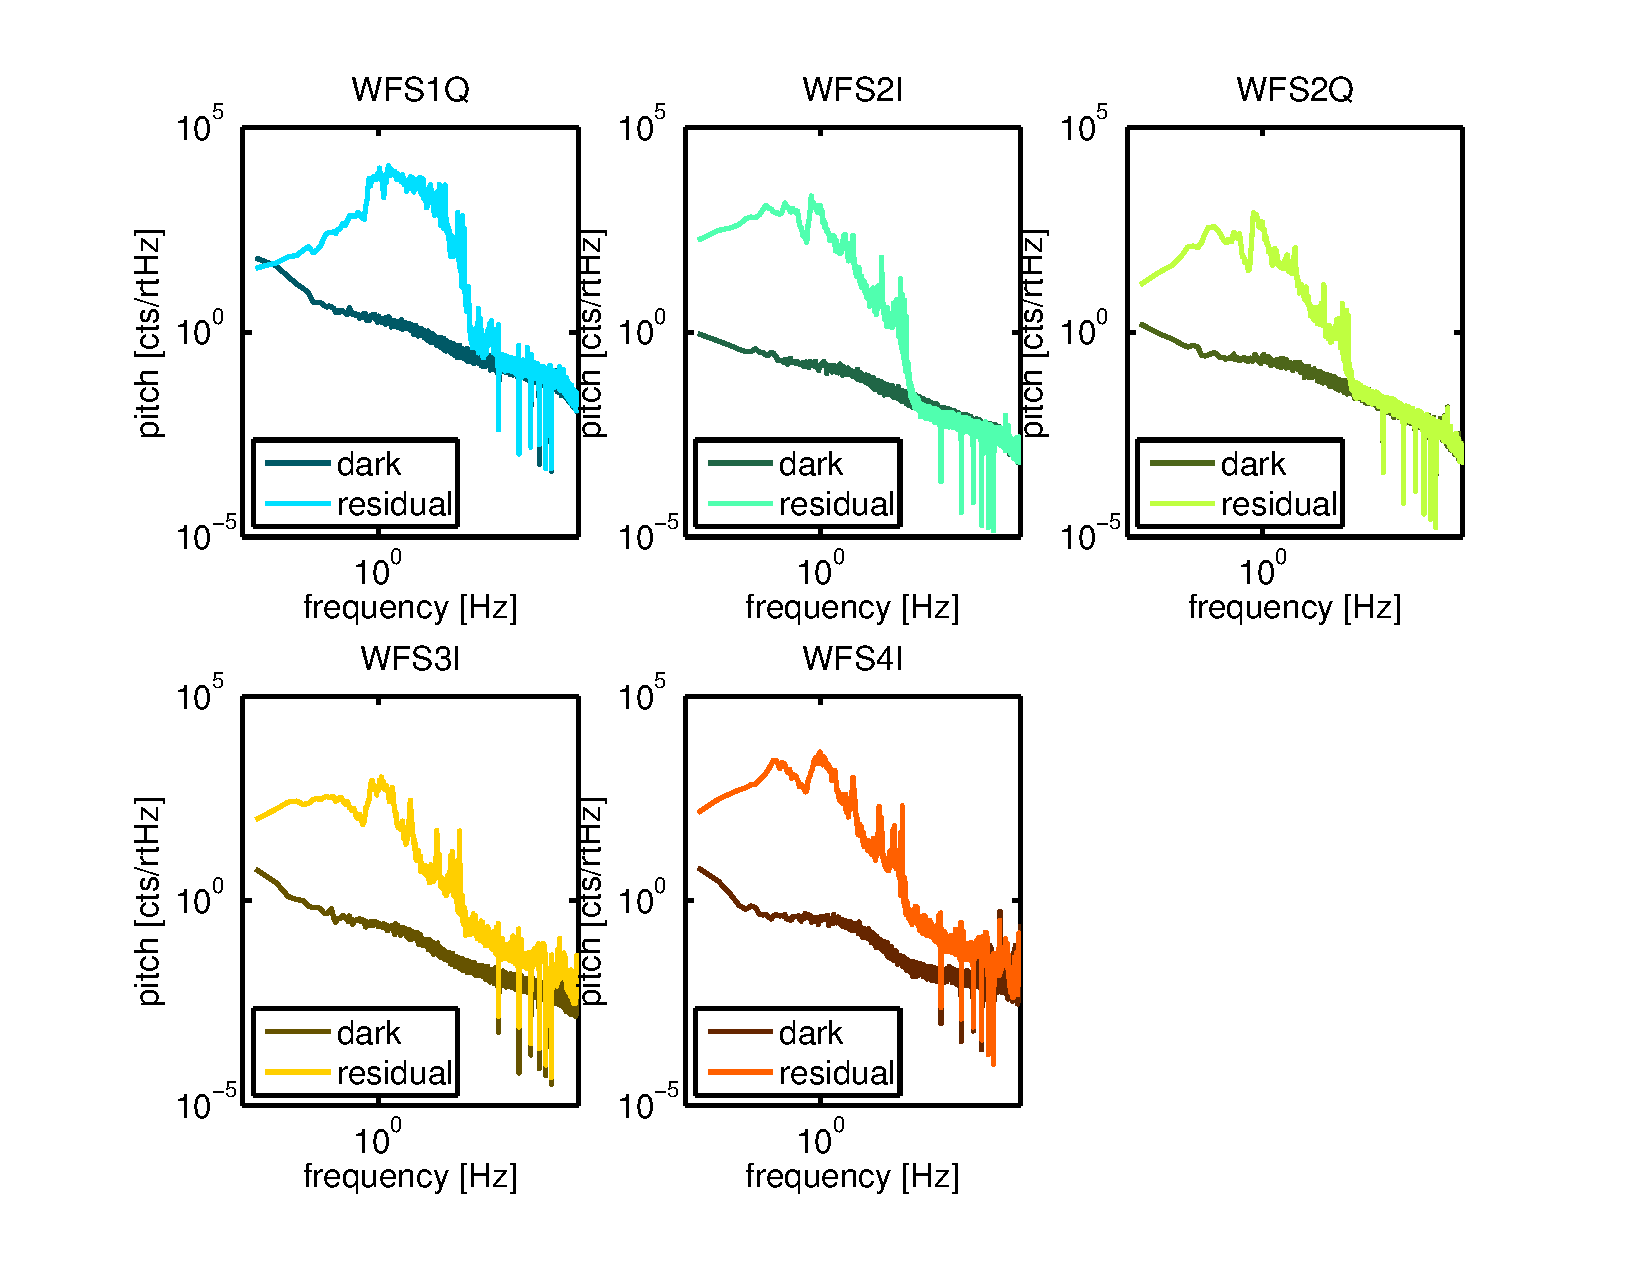
\includegraphics[width=1.0\textwidth]{figures/ASCsensorsignals.pdf} 
\caption[WFS error signal and dark noise]{WFS dark noise compared to typical error signal. \textcolor{blue}{Include shot noise, too, especially for WFS1.} The excess signal above the dark noise in WFS3I and WFS4I from 20~Hz on is likely acoustic noise, although this has not been verified. WFS1 and WFS2 are on a floating table in a sound proof chamber, while WFS3 and WFS4 are on a non-seismically isolated table without a sound proof enclosure.}
\label{fig:WFSdarknoise}
\end{centering}
\end{figure}

Besides the sensing noise, there is also sometimes real signal that results in more harm than good when used as feedback. The HAM seismic isolation tables used by the Input Optics (the core optics are suspended from BSC tables) have stack modes of xx Hz that ring up the MMTs.  At low frequencies, around 1~Hz, some of the WFS signals are dominated by these angular fluctuations of the input beam. The resulting attempt of the mirrors to follow the input beam jitter leads to a magnification of the motion because of the drastically different length scales. Large power fluctuations in both arms and the power recycling cavity ensue, leading to departure from the linear error signal regime and often lock loss. 

Other limitations to the reduction of mirror motion result from the nature of control loops. The cut-off filter, for example, reduces the phase margin of the open loop gain, necessarily pushing down the unity gain frequency (UGF) and therefore the magnitude of suppression at all frequencies below the UGF. A less aggressive cut-off filter, while improving the servo's stability and allowing for higher overall gains, leads to more impression of sensing noise on the optics. Also, when the phase margin of the loop is low, some mirror motion is amplified through gain peaking.

% A final point that should be noted, but is in fact insignificant, is a coupling from angular drive to length that results from the same principle of the length to angle coupling presented in \ref{sec:L2A}. 

% We will show that we don't quite meet all of these requirements and the impression of sensing noise in fact plays a major role in the reduction of DARM sensitivity up to 70 Hz.



\section{Wavefront sensing}
\label{sec:wfs}
Describe modes, reference sidebands, Gouy phases; give FP cavity example. 





\chapter{Dynamic response of coupled pendula}
In order to design a control system that reduces the angular motion of
the interferometer mirrors to the levels necessary for stable
interferometer operation and minimal impact on strain sensitivity, the
angular response of the mirrors to external torque must be fully
understood. The suspended mirrors themselves are nothing more than
torsion pendula. However, the torque induced by radiation pressure
couples the angular motion of the mirrors in a power dependent way,
complicating the plant for which controls must be designed. Namely,
radiation pressure torque has the effect of breaking the symmetry of
the equations of motion of each of the mirrors. Since Enhanced LIGO
embarks on the path of increasing the laser power, examining the
effect of radiation pressure torque in detail is warranted. Here, we
review the dynamics of a torsion pendulum and the geometry of a linear
cavity, and conclude with the derivation and implications of a set of
eigenfunctions that diagonalize the linear cavity's response to
radiation pressure. The torque to angle transfer functions of the new
eigenmodes are modified such that one mode is statically unstable at
Enhanced LIGO powers. 



\section{The mirror as a torsion pendulum}
\label{sec:pendTF}
The mirrors in LIGO may be regarded as torsion pendula. Each mirror is
suspended from a single \textcolor{blue}{xx m diameter} wire that
loops around the bottom of the barrel of the mirror as shown in
Fig. \ref{fig:suspension}. Stand-offs glued just above the mirror's
center of mass on both sides of the barrel mark the final point of
contact of the wire with the mirror, and both ends of the wire are
clamped to the top of a suspension cage. The mirror is free to twist
an angle $\theta$ about a horizontal axis passing through its center
of mass to create motion in \emph{pitch} and about a vertical axis
passing through its center of mass to create a motion in \emph{yaw}.

The angular equation of motion of the mirror is governed by the sum of
all torques on the mirror. First, let's consider the most simplistic
scenario where there is only a pendulum restoring torque
$\tau_p=-\kappa_p \theta$, where $\kappa_p$ is the pendulum's
torsional constant. The equation of motion is
\begin{equation}
I \ddot{\theta} + \kappa_p \theta = 0,
\end{equation}
which has a solution of $\theta(t) = \sin({\omega_0 t)}$, where
$\omega_0 = \sqrt{\kappa_p/I}$ is the resonant angular frequency and
$I$ is the mirror's moment of inertia. The pendulum torsional constant
serves to make the mirror oscillate indefinitely about its equilibrium
position upon the slightest of displacements.

\begin{figure}
\begin{centering}
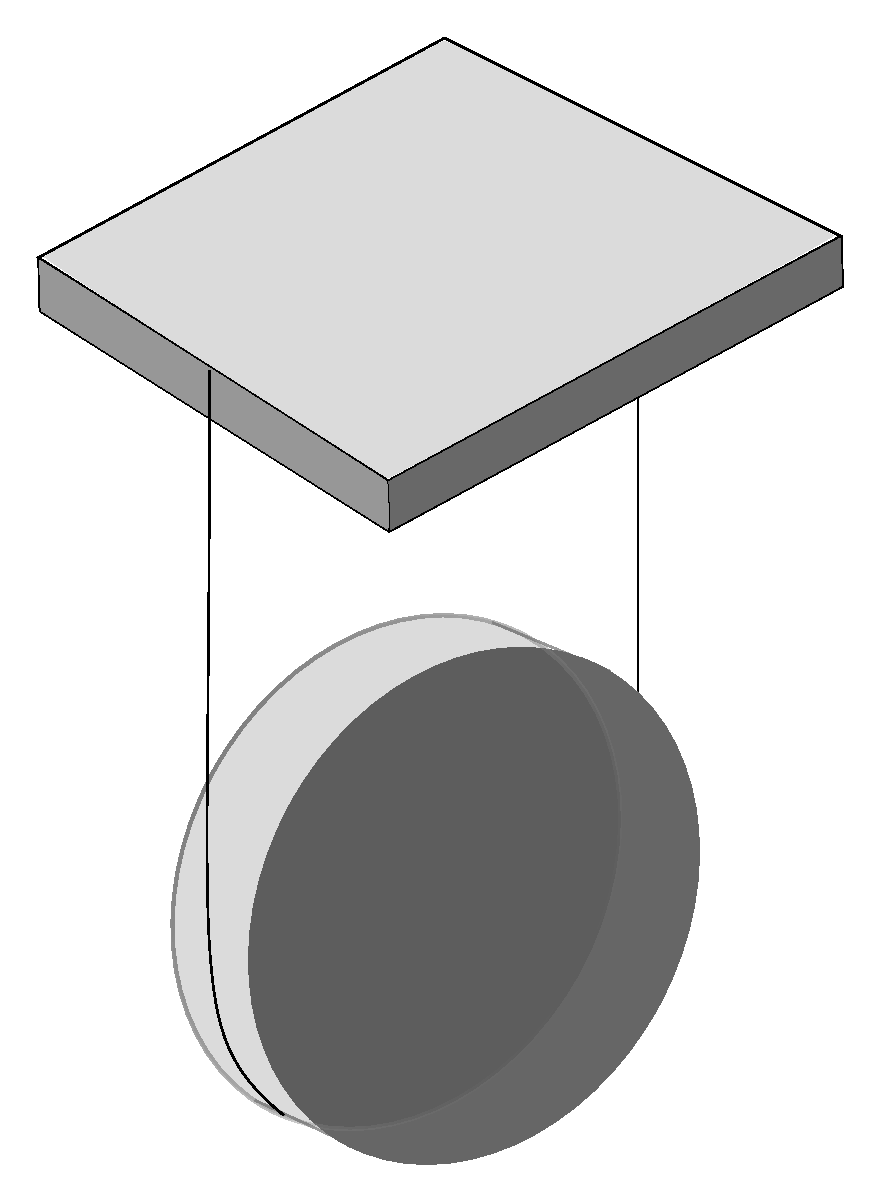
\includegraphics[width=0.3\textwidth]{/Users/kate/kate-thesis/figures/suspension.pdf}
\caption[Sketch of a LIGO suspension]{Cartoon of a LIGO
  suspension. \textcolor{blue}{Improve this.}}
\label{fig:suspension}
\end{centering}
\end{figure}




\subsection{Torque to angle transfer function of a pendulum}
\label{sec:t2a}
We are particularly interested in the pendulum's response to an
external torque, such as seismic noise. In order to calculate the
torque to angle transfer function, we must include an external torque
term, $\tau_{ext}$, in the equation of motion:
\begin{equation}
I \ddot{\theta} + \gamma \dot{\theta} + \kappa_p \theta = \tau_{ext}.
\label{eq:eqmotion}
\end{equation}
Here, we have also introduced a velocity damping term, $\gamma$, to
best model reality. Taking the Laplace transform to convert from the
time domain to the frequency domain, we have:
\begin{equation}
I s^2 \Theta + \gamma s \Theta + \kappa_p \Theta = \tau_{ext}
\end{equation}
where $s$ is a complex parameter. The transfer function is then
defined as
\begin{equation}
H(s) := \frac{\Theta(s)}{\tau_{ext}(s)} = \frac{1}{I s^2 + \gamma s + \kappa_p}.
\label{eq:TF}
\end{equation}
We are only interested in examining the transfer function for a pure
sine wave excitation, $e^{i\omega t}$, so we substitute $s=i\omega$ to
get
\begin{equation}
H(\omega) = \frac{1/I}{\omega_0^2  - \omega^2 + i \gamma \omega / I}.
\end{equation}
The resonant frequency of this damped system can be computed by finding the
$\omega$ at which the amplitude of the transfer function, $[I^2
[\omega^2 - \omega_0^2]^2 + \gamma^2 \omega^2]^{-1/2}$, is maximized:
\begin{equation}
\omega_{res} = \sqrt{\omega_0^2 - \frac{\gamma^2}{2I^2}}.
\end{equation}
We note that damping serves to reduce the resonant frequency.

A quantity that is more familiar than $\gamma$ for describing the
losses of a system with a real resonance is the quality factor,
$Q~:=~\omega_{res}/\mathrm{FWHM}$, where FWHM is that computed for the
amplitude squared of the transfer function. When the losses are small,
$\omega_{res} \approx \omega_0$ and FWHM $\approx \gamma/I$ (see
Feynman 23-4). The quality factor is then well approximated by $Q =
\sqrt{\kappa_p I}/\gamma$. The transfer function written in terms of
$Q$ is
\begin{equation}
H(\omega) = \frac{1/I}{\omega_0^2  - \omega^2 + i \omega \omega_0 / Q}.
\label{eq:TFpendulum}
\end{equation}

Figure \ref{fig:pendTF} shows the pendulum torque to angle transfer
function (for pitch) using the parameters of a LIGO core optic. For
external torques applied to the mirror above its resonant frequency,
the mirror acts like a free mass, one that is not held in place by
suspension wires nor subject to damping. For torques applied to the
mirror below its resonant frequency, the mirror's angle is determined
by the inverse of the torsional constant.

\begin{figure}
\begin{centering}
\includegraphics[width=1.0\textwidth]{figures/pendTF.pdf}
\caption[Torque to pitch transfer function of a LIGO core
optic]{Torque to pitch transfer function of a LIGO core optic
  (blue). The optic acts like a free mass at high frequencies (red)
  and the DC magnitude of the transfer function is determined by the
  inverse torsional constant (green). A damping constant $\gamma =
  0.006$ ($Q=32$) was selected for pictorial representation only. The
  resonant frequency of LIGO core optics in yaw is 0.5~Hz.}
\label{fig:pendTF}
\end{centering}
\end{figure}




\section{The radiation pressure angular spring}
The geometric axis of a cavity formed by two spherical mirrors is
dictated by the line joining the centers of the ``spheres'' created by
the two mirrors. Only if the mirrors are pointed directly at one
another will the cavity axis pass through the centers of the
mirrors. Should a laser beam resonate in the cavity, it will do so
along this geometric axis. Thus, if the mirrors are tilted away from
one another, the beam spot on each mirror will not be centered. The
relationship between the positions of the beams on the mirrors
relative to center, $x_i$, and the angles of the mirrors, $\theta_i$,
is given by:
\begin{equation}
\left\llbracket \begin{array}{c}
x_1\\
x_2 \end{array} \right\rrbracket = \frac{L}{1-g_1 g_2}
\left\llbracket \begin{array}{cc}
g_2 & 1\\
1 & g_1\end{array} \right\rrbracket
\left\llbracket \begin{array}{c}
\theta_1\\
\theta_2 \end{array} \right\rrbracket .
\label{eq:x}
\end{equation}
The $g$-factor is defined as $g_i=1-R_i/L$ where $R_i$ is the radius of
curvature of each of the mirrors, respectively, and $L$ is the length
of the cavity.

We saw in the previous chapter that the radiation pressure torque on a
mirror depends on the position of the beam on the mirror, $\tau_{rp} =
2 P x / c$ (Eq. \ref{eq:tau_rp}). Based on Eq. \ref{eq:x} the
radiation pressure torque on a mirror that is part of a
Fabry-P\'{e}rot cavity is therefore dependent on the angle of both the
mirror of interest and the second mirror forming the cavity:
\begin{equation}
\left\llbracket \begin{array}{c}
\tau_{rp,1}\\
\tau_{rp,2} \end{array} \right\rrbracket = \frac{2 P L}{c (1-g_1 g_2)}
\left\llbracket \begin{array}{cc}
g_2 & 1\\
1 & g_1\end{array} \right\rrbracket
\left\llbracket \begin{array}{c}
\theta_1\\
\theta_2 \end{array} \right\rrbracket.
\end{equation}
This is more succinctly expressed as
\begin{equation}
\vec{\tau}_{rp} = -\mathbf{K_{rp}} \vec{\theta},
\label{eq:rpspring}
\end{equation}
where $\mathbf{K_{rp}}$ is the \emph{torsional stiffness
  matrix}. Equation \ref{eq:rpspring} is the expression that describes
the radiation pressure angular spring.




\subsection{Diagonalizing the modified equations of motion}
\label{sec:eigenbasis}
The radiation pressure spring modifies the pendulum angular equation
of motion and therefore the torque to angle transfer function
through the addition of an angle-dependent torque term. Re-writing
Eq. \ref{eq:eqmotion} in matrix form and with the radiation pressure
spring term, the two equations that describe the motion of two mirrors
forming a Fabry-P\'{e}rot cavity is: 
\begin{equation}
\mathbf{I} \ddot{\vec{\theta}} 
+ {\bm \gamma} \dot{\vec{\theta}} 
+ \mathbf{\kappa_p} \vec{\theta}
- \frac{2 P L}{c (1-g_1 g_2)}
\left\llbracket \begin{array}{cc}
g_2 & 1\\
1 & g_1\end{array} \right\rrbracket \vec{\theta} 
= \vec{\tau}_{ext}.
\label{eq:motion_rp}
\end{equation}
$\mathbf{I}$, $\gamma$, and $\kappa_p$ are $2 \times 2$ diagonal
matrices and $\vec{\theta}$ and $\vec{\tau}_{ext}$ are $2 \times 1$
vectors as in the previous section. Due to the non-diagonal matrix in
Eq. \ref{eq:motion_rp}, the motions of each of the mirrors forming the
cavity are tied to one another. The natural way to work with such a
system is to rotate the coupled equations into a new basis. The
resulting de-coupled equations of motion will described specific
combinations of mirror tilts instead of individual mirrors. Vectors in
the rotated basis are written with primes.

In order to decouple the two equations of Eq. \ref{eq:motion_rp}, we
need to diagonalize $\mathbf{K_{rp}}$. The subscripts $a$ and $b$ are
used to denote the elements of the diagonalized basis, to contrast the
$1$ and $2$ which denote the mirror basis. Ignoring the constants of
matrix $\mathbf{K_{rp}}$, its eigenvalues are
\begin{align}
\lambda_a &= \frac{g_1 + g_2 + \sqrt{(g_1 - g_2)^2 + 4}}{2} \\
\lambda_b &= \frac{g_1 + g_2 - \sqrt{(g_1 - g_2)^2 + 4}}{2} 
\label{eq:eigenvalues}
\end{align}
and its eigenvectors are
\begin{align}
\vec{v}_a &= \left\llbracket \begin{array}{c} 
1 \\
\frac{g_1 - g_2 + \sqrt{(g_1 - g_2)^2 + 4}} {2} \end{array} \right\rrbracket\\
\vec{v}_b &= \left\llbracket \begin{array}{c}
\frac{ -g_1 + g_2 - \sqrt{(g_1 - g_2)^2 + 4}}{2} \label{eq:eigenvectors}\\
1 \end{array} \right\rrbracket .
\end{align}
Therefore, the matrix 
\begin{equation}
\mathbf{S} = \left\llbracket \begin{array}{cc} 
\vec{v}_a & \vec{v}_b \end{array} \right\rrbracket =
\left\llbracket \begin{array}{cc}
 1 & \frac{-g_1 + g_2 - \sqrt{(g_1 - g_2)^2 + 4}} {2}\\
 \frac{g_1 - g_2 + \sqrt{(g_1 - g_2)^2 + 4}} {2} & 1\end{array} \right\rrbracket
\end{equation}
diagonalizes $\mathbf{K_{rp}}$ such that 
\begin{equation}
\mathbf{S^{-1} K_{rp} S} = \mathbf{D} = \left\llbracket \begin{array}{cc} 
\lambda_a & 0 \\
0 & \lambda_b \end{array} \right\rrbracket = \left\llbracket \begin{array}{cc}
 \frac{g_1 + g_2 + \sqrt{(g_1 - g_2)^2 + 4}}{2}  & 0\\
 0 & \frac{g_1 + g_2 - \sqrt{(g_1 - g_2)^2 + 4}}{2}\end{array}
\right\rrbracket .
\label{eq:diag}
\end{equation}
The matrix of eigenvectors, $\mathbf{S}$, is the basis transformation
matrix. It serves to define the torque and angle vectors in the new
basis. For example,
\begin{equation}
\vec{\theta}^\prime = \left\llbracket \begin{array}{c}
\theta_a\\
\theta_b \end{array} \right\rrbracket = \mathbf{S^{-1}}
\left\llbracket \begin{array}{c}
\theta_1\\
\theta_2 \end{array} \right\rrbracket
= \mathbf{S^{-1}} \vec{\theta}.
\end{equation}

Rearranging Eq. \ref{eq:diag} to the form $\mathbf{K_{rp}} =
\mathbf{S D S^{-1}}$ and substituting it into Eq. \ref{eq:motion_rp},
we have:
\begin{equation}
\mathbf{I} \ddot{\vec{\theta}} 
+ {\bm \gamma} \dot{\vec{\theta}} 
+ \mathbf{\kappa_p} \vec{\theta}
- \frac{2 P L}{c (1-g_1 g_2)} \mathbf{S D S^{-1}} \vec{\theta} 
= \vec{\tau}_{ext} 
\end{equation}
Multiplying on the left by $\mathbf{S}$, taking advantage of the
diagonal $\mathbf{I}$, $\gamma$, and $\kappa_p$ matrices, and using
$\mathbf{S}$ to change the basis of each of the vectors, the
de-coupled equations of motion are:
\begin{equation}
\mathbf{I} \ddot{\vec{\theta}}^\prime 
+ {\bm \gamma} \dot{\vec{\theta}}^\prime 
+ \mathbf{\kappa_p} \vec{\theta}^\prime
- \frac{2 P L}{c (1-g_1 g_2)}
\left\llbracket \begin{array}{cc}
\lambda_a & 0\\
0 & \lambda_b \end{array} \right\rrbracket \vec{\theta}^\prime 
= \vec{\tau}_{ext}^\prime.
\label{eq:rp_eqmotion}
\end{equation}
The radiation pressure spring constant, $\kappa_{rp}$, is 
\begin{equation}
\kappa_{rp} = - \frac{2 P L}{c (1-g_1 g_2)} \lambda
\end{equation}
where $\lambda = \lambda_a$ or $\lambda_b$, depending on the mode in
question. 

The angular motion of the Fabry-P\'{e}rot cavity is no longer
described on an individual mirror basis. Due to radiation pressure,
the cavity is treated as a unit and the two orthogonal modes of
angular motion are combinations of the two mirrors' angles. The
eigenvectors $\vec{v}_a$ and $\vec{v}_b$ describe these two sets of
orthogonal mirror tilts, and the eigenvalues $\lambda_a$ and
$\lambda_b$ (along with their common constants) quantify the magnitude
of the radiation pressure torsional spring constant for each of the
modes. While the equations of motion had been identical for each of
the individual mirrors, the decoupled equations in the presence of
radiation pressure breaks that symmetry.


\begin{table}
\centering
\caption[Geometric parameters of the LIGO arm cavity
  eigenmodes]{Geometric parameters of the LIGO arm cavity
  eigenmodes. $x_i$ are the beam locations on the mirrors relative
  to center, $a$ is the cavity axis displacement at the waist, and
  $\alpha$ is the cavity axis angle with respect to a line joining the
  centers of the mirrors. Differences between LLO and LHO arise from the
  mirrors at each site having different radii of curvature. Quantities
  are expressed as a function of the amount of tilt in a particular mode.}
\begin{tabular}{l l l l l l}
& & LLO & LLO & LHO & LHO \\
cavity parameter & unit & $\vec{v}_a$ mode & $\vec{v}_b$ mode & $\vec{v}_a$ mode & $\vec{v}_b$ mode \\
\hline\hline
$|x_1|$ & mm/urad & 9.88 & 2.44 & 8.20 & 2.51\\
$|x_2|$ & mm/urad & 10.84 & 2.22 & 9.35 & 2.20\\
$|a|$ & mm/urad & 10.17 & 1.01 & 8.48 & 1.34 \\
$|\alpha|$ & urad/urad & 0.24 & 1.17 & 0.29 & 1.18 \\
\hline
\end{tabular}
\label{table:cav_geometric}
\end{table}


Table \ref{table:cav_geometric} outlines the characteristics of these
two eigenmodes for the specific geometry of the LIGO arm cavities. The
amount of beam displacement on each mirror is given as a function of
the amount of tilt in one eigenmode or the other. Furthermore, the
amount of cavity axis displacement $a$ and cavity axis tilt $\alpha$
is also calculated for each eigenmode using the geometric relationship
between a set of mirror tilts and their cavity axis as derived in
Appendix \ref{sec:misaligned_cavity}. Figure \ref{fig:ss} illustrates
a cavity in each of the two eigenmodes when using the parameters from
Table \ref{table:cav_geometric}.


\begin{figure}
\begin{centering}
\includegraphics[width=0.6\columnwidth]{figures/eigenmodes.pdf}
\caption[Illustration of the orthogonal modes of cavity
tilt]{Illustration of the orthogonal modes of cavity tilt. The upper
  diagram shows tilts given by eigenvector $\vec{v}_b$ and the lower
  diagram shows $\vec{v}_a$. \textcolor{blue}{Labels.}}
\label{fig:ss}
\end{centering}
\end{figure}




\subsection{Soft and hard modes} 
The torque to angle transfer function of each of these eigenmodes has
the same form as that of a single pendulum (Eq. \ref{eq:TF}), but the
spring constant is modified. More importantly, the spring constant is
modified differently for each mode, yielding distinct behaviors of the
two eigenmodes. In this section, we analyze these behaviors and
accordingly introduce the names \emph{soft} and \emph{hard} to use in
place of $a$ and $b$ for describing the two modes.

Just as in Sec. \ref{sec:t2a}, we can take the Laplace transform of
each of the equations in Eq. \ref{eq:rp_eqmotion} to get the general
form of the modal torque to angle transfer function:
\begin{equation}
H^\prime(s) = \frac{\Theta^\prime(s)}{\tau_{ext}^\prime(s)} = \frac{1}{I s^2 + \gamma s +
  \kappa_p + \kappa_{rp}}.
\label{eq:modalTF}
\end{equation} 
Figure \ref{fig:pendloop} shows the control theory view of
the addition of the radiation pressure spring constant to the transfer
function.

\begin{figure}
\begin{centering}
\includegraphics[width=0.6\textwidth]{figures/pendulumLoop.pdf}
\caption[Controls view of addition of radiation pressure to the pendulum
transfer function]{Demonstration of how radiation pressure modifies the torque to
  angle transfer function of a Fabry-P\'{e}rot cavity's eigenmodes.}
\label{fig:pendloop}
\end{centering}
\end{figure}

The magnitude and sign of the total torsional spring constant,
$\kappa_{tot} = \kappa_p + \kappa_{rp}$, conveys critical information
about the stability of the cavity and the nature of its response to
external torque. Recalling the equation of an angular spring, $\tau =
- \kappa_{tot} \theta$, a restoring torque is provided only if
$\kappa_{tot} > 0$, which is equivalent to the condition for
stability. If $\kappa_{tot} < 0$, the spring is an anti-spring,
resulting in an unstable, run-away situation. Furthermore, 
while $\kappa_{tot}$ is positive, its magnitude directly relates to
the stiffness of the spring.

The stability criteria for the coupled cavity eigenmodes 
depend on the relationship between $\kappa_p$ and $\kappa_{rp}$:
\begin{align}
\mbox{stable: } k_{tot} > 0 \implies & \frac{2 P L}{c (1-g_1 g_2)} \lambda < \kappa_p \\
\mbox{unstable: } k_{tot} < 0 \implies & \frac{2 P L}{c (1-g_1 g_2)} \lambda > \kappa_p.
\label{eq:stability}
\end{align}
The pendulum spring constant, $\kappa_p$, is always positive, so we
can conclude with certainty that the cavity eigenmode is stable as
long as the quantity on the left-hand side of Eq. \ref{eq:stability}
is negative. However, if this quantity is positive, then its magnitude
compared to $\kappa_p$ determines stability. Since $P$, $L$, and $c$
are all positive numbers and the g-factor is restricted to $0 < g_1g_2
< 1$ \footnote{This is the necessary condition for a two mirror
  resonator to form a stable periodic focusing
  system. \cite[p. 747]{Siegman1986Lasers}}, the sign of the left-hand
side is determined solely by that of $\lambda$. From the g-parameter
restriction, it can be shown that $\lambda_a$ is always positive and
that $\lambda_b$ is always negative. Therefore, the mode whose mirror
angles are described by $\vec{v}_a$ is either stable or unstable, and
the mode described by $\vec{v}_b$ will always be stable.

The precise situation for the potentially unstable mode depends on the
one non-constant variable, the circulating power $P$. There is a
critical power at which $\kappa_{rp}$ = - $\kappa_p$, and at any
greater power, instability ensues. In general, as power increases, the
total spring constant for the potentially unstable mode decreases,
creating a softer spring, and the total spring constant for the
unconditionally stable mode increases, creating a stiffer spring. Thus
arise the terms \emph{soft} and \emph{hard} to describe the two
eigenmodes that have been referred to by $\vec{v}_a$ and $\vec{v}_b$,
respectively.

\begin{figure}
\begin{centering}
\includegraphics[width=1.0\textwidth]{figures/khardsoftLLO.pdf}
\caption[Torsional spring constants of an optically coupled
  cavity]{Torsional spring constants (pitch) of an optically coupled
  cavity for LLO parameters. The soft mode is unstable when the spring
  constant is negative.}
\label{fig:k_hardsoft}
\end{centering}
\end{figure}

Figure~\ref{fig:k_hardsoft} shows the dependence of $\kappa_{tot}$ on
circulating power for the soft and hard modes of a LIGO arm
cavity. Without power in the cavity, the modes are identical and their
spring constants are simply that of the individual pendula. The
symmetry-breaking effect of radiation pressure comes into play as soon
as light resonates in the cavity: the hard mode's spring constant
increases and the soft mode's spring constant decreases. The critical
power at which the soft mode becomes unstable is 10~kW, which
corresponds to approximately 6~W input power (for Enhanced LIGO
efficiencies) to the interferometer. Above the critical power,
radiation pressure creates an optical anti-spring. 

Table \ref{table:k_tot} highlights the values of the spring constants
for the typical power that was used in Initial LIGO (9~kW) and for the
highest of powers achieved in Enhanced LIGO (40~kW). The corresponding
transfer functions for these spring constants is found in
Fig. \ref{fig:optomechhardsoft}. The resonant frequency, $\omega_0 =
\sqrt{\kappa_{tot}/I}$, increases with power for the hard modes and
decreases for the soft modes. Once $\kappa_{tot}$ becomes negative, as
is the case for the Enhanced LIGO soft mode, there is no real resonant
frequency.


\begin{table}
\centering
\caption[Torsional spring constants for the soft and hard cavity modes]{Torsional spring constants (pitch) for the soft and hard modes of a typical
  Initial LIGO power and the highest of Enhanced LIGO powers. The soft
  mode in Enhanced LIGO is unstable. The $\kappa_p$ values assume a
  resonant frequency of 0.6~Hz.}
\begin{tabular}{l l l l l}
\hline
 & $P_{circ}$ & $\kappa_{p}$ & $\kappa_{tot}$, soft mode &
 $\kappa_{tot}$, hard mode\\
% & (kW) & (Nm/rad) & (Nm/rad) & (Nm/rad) \\
\hline
Initial LIGO & 9 kW & 0.721 Nm/rad& 0.0734 Nm/rad & 0.867 Nm/rad\\
Enhanced LIGO & 40 kW & 0.721 Nm/rad& -2.18 Nm/rad & 1.38 Nm/rad\\
\hline
\end{tabular}
\label{table:k_tot}
\end{table}

\begin{figure}
\begin{centering}
\subfigure{\includegraphics[width=1.0\textwidth]{figures/ieLIGOTFmags.pdf}}
\subfigure{\includegraphics[width=1.0\textwidth]{figures/ieLIGOTFphases.pdf}}
\caption[Single cavity opto-mechanical transfer function]{Single
  cavity opto-mechanical transfer function for pitch. The resonant
  frequency increases with power for the hard mode, but decreases for
  the soft mode, eventually becoming imaginary. $P_{circ} = 9$ kW
  (5.25 W input) was a typical operating power for Initial LIGO and
  $P_{circ} = 40$ kW (23.5 W input) is the highest of powers reached
  for Enhanced LIGO.}
\label{fig:optomechhardsoft}
\end{centering}
\end{figure}


One final comment about the analysis of the modified transfer function
(Eq. \ref{eq:modalTF}) is that the two poles,
\begin{equation}
s = s_\pm = \frac{-\gamma \pm \sqrt{\gamma^2 - 4 I \kappa_{tot}}}{2 I},
\label{eq:TFpoles}
\end{equation}
provide an additional \textcolor{blue}{(find better word)} way to view
the stability of the system. As long as the poles are negative, the
impulse response will decay or be sinusoidal. However, if a pole is
positive, the system's motion will experience exponential growth. The
constraints for $s_\pm$ to be in a particular half of the s-plane are
easily derived from Eq. \ref{eq:TFpoles}. Note that $s_-$ will always
be in the left half of the plane and that $s_+$ is the pole that has
the potential of falling in the right half of the plane. Table
\ref{table:s_0} show how the s-plane locations for $s_+$ depend on
$\kappa_{tot}$. The sign of $\kappa_{tot}$ determines stability, as
expected, and we see that the nature of the stable response depends on
the damping coefficient. Figure \ref{fig:TFrainbow_poles} plots the
pole locations for a range of $\kappa_{tot}$ experienced while
powering up Enhanced LIGO.

% \begin{figure}
% \begin{centering}
% \subfigure{\includegraphics[width=1.0\textwidth]{figures/TFrainbow_mags.pdf}}
% \subfigure{\includegraphics[width=1.0\textwidth]{figures/TFrainbow_phases.pdf}}
% \caption{Magnitude and phase of the torque to pitch transfer function
%   as a function of torsional constant for a fixed damping coefficient
%   of $\gamma^2/4I = 1.77 \times 10^{-4}$. This range of $\kappa$
%   represents the torsional constants experienced while powering up
%   Enhanced LIGO.}
% \label{fig:TFrainbow}
% \end{centering}
% \end{figure}

\begin{table}
\centering
\caption[Conditions on total torsional constant for determining system stability]{Conditions on total torsional constant $\kappa_{tot}$ for determining
  system stability.}
\begin{tabular}{l l l}
$\kappa_{tot}$ condition & pole $s_+$ & impulse response \\
\hline\hline
$\kappa_{tot} < 0$ & real positive & statically unstable\\
$\kappa_{tot} = 0$ & zero & \\
$0 < \kappa_{tot} < \gamma^2/4I $ & real negative & stable decay \\
$\kappa_{tot} > \gamma^2/4I$ & real negative, and imaginary & stable,
oscillatory \\
\hline
\end{tabular}
\label{table:s_0}
\end{table}


\begin{figure}
\begin{centering}
\includegraphics[width=0.667\textwidth]{figures/TFrainbow_poles.pdf}
\caption[Poles of the torque to pitch opto-mechanical transfer
function]{Poles of the torque to pitch transfer function as a function
  of torsional constant, $\kappa_{tot}$. Crosses show $s_+$ and
  asterisks show $s_-$. Poles in the right half of the s-plane
  indicate the system is unstable.}
\label{fig:TFrainbow_poles}
\end{centering}
\end{figure}



\section{Implications}
These are the transfer functions for which controls must be designed.




\section{ASC loops}

\subsection{Optical lever servo compensation}




\chapter{Angular sensing and control characterization and performance in the radiation pressure eigenbasis} 





The Enhanced LIGO goal of increasing the input power to 30 W from the
Initial LIGO 7 W makes radiation pressure torques cross into the realm
of significance. In particular, the soft opto-mechanical mode which
approached instability for Initial LIGO powers actually becomes
unstable for Enhanced LIGO powers. The static instability requires
high DC gain. The sensors in Initial LIGO, however, were not tuned in
to specifically look for the combined mirror motions that create the
unstable mode. The only way to provide adequate DC control to prevent
the mirrors from falling apart would be to increase the gain of all of
the angular control loops. Since some of the sensors are less good
than others, this would result in extreme impression of noise on
DARM. Thus, to maintain a reasonable noise budget while reigning in
the static instability, we need to make the sensors specifically pick
out the mirror motions that together create this detrimental
mode. This is the basis of the ASC work for Enhanced LIGO--switching
the sensors to the radiation pressure eigenmode basis, and increasing
the gain of the single loop that is sensitive to only the unstable mode. 

In this chapter I show how the angular displacements are sensed and
why control filters implemented in the eigenbasis of radiation
pressure torques is best. 



% \section{Sensing}
% There are five main subsets of sensor systems for the ASC:
% \begin{itemize}
% \item OSEMs
% \item optical levers (MMT3, RM, BS, ITMX, ITMY, ETMX, ETMY) \vspace{-10pt}
% \item camera image (BS)
% \item quadrant photodiodes (QPDX, QPDY) \vspace{-10pt}
% \item wavefront sensors (WFS1, WFS2, WFS3, WFS4) \vspace{-10pt}
% \end{itemize}
% Together, these sensors need to provide enough information to derive
% adequate control signals for 9 mirrors in both pitch and yaw. Both
% absolute motion (AC) and relative motion (DC) need to be
% suppressed. The OSEMs and optical levers provide local AC control to
% the mirrors. The video camera and the QPDs control the pointing of the
% input beam; the video camera works at DC and the QPDs at both DC and
% AC. The WFS provide the top level fine tuning of DC and AC control to
% the 5 main mirrors.


% \subsection{OSEMs}
% The most basic level of control is local damping of each suspended
% optic provided by the OSEMs. This is always on, even when the
% interferometer loses lock. It works by sending current through the
% OSEM coils to keep a constant amount of light on the OSEM shadow
% sensor.


% \subsection{Optical levers}
% The optical levers are local to each large optic and provide a record
% at all times of pitch and yaw pointing of each mirror with respect to
% the ground. The mirrors are velocity-damped only by the optical
% levers; they are not controlled at DC. The optical lever is a HeNe
% laser beam that reflects off of the mirror and onto a QPD. Both the
% laser and QPD are mounted on heavy piers to reduce the seismic noise
% contribution to the QPD signal. The optical lever provides a feedback
% signal to the mirror's coils to reduce the sensed motion. Each large
% optic has its own independent optical lever loop which is almost
% always on, even when the interferometer is out of lock. The optical
% lever loops provide the second level of controlled stabilization of
% the mirrors, after only the local damping.


% \subsection{Camera image}
% The most primitive sensor is that of the physical video camera.  The
% video camera monitors the location of the spot on the beam splitter,
% thus serving as a sensor of the pointing of the input beam. The image
% of the speckle of light reflected off of the beam splitter (see
% Fig. \ref{fig:BCS}) is fed into a labview program which integrates the
% intensity of the image to identify the coordinates of the center of
% the beam spot. This is compared with a hardcoded desired center
% location and a mirror upstream, MMT1 is moved to redirect the input
% beam, minimizing the difference between the desired and actual beam
% spot location on the BS.

% \begin{figure}
% \begin{centering}
% \includegraphics[width=0.8\textwidth]{figures/BCSspiricon.pdf}
% \caption{Image of beam on beam splitter as used for the beam centering servo.}
% \label{fig:BCS}
% \end{centering}
% \end{figure}


% \subsection{QPDs}  
% QPDX and QPDY see the small amount light that is transmitted through
% the ETMs, providing a monitor of the modal axes of the arm cavities. Together with the , they maintain the alignment of the input . QPDX 


% \subsection{WFSs}  
% The wavefront sensors provide the most sophisticated form of
% measuring angular motion of the mirrors. Their frame of reference is
% the fundamental Gaussian mode of the interferometer cavities (x-arm,
% y-arm, recycling cavity) as aligned to ???. All of the mirrors
% globally follow the pointing of the input beam (via the QPDs) which is
% in turn stabilized to the center of the beam splitter (via the BCS) at frequencies well
% below the pendulum resonances. The job of the wavefront sensors is to
% keep the mirrors aligned to one another up to several Hz within this
% hierarchy of alignment. The WFS provide DC and AC control to the
% mirror angles. 




% \section{Control}
% When the gain is really high, comparing the calibrated error and
% control signals shows just what the control loop is doing. The error
% is the residual and the control is what there would be without the
% loop.

% error * (1+G) is the motion without the loop, where G is the open loop gain.

% \begin{itemize} 
% \item optical lever calibration
% \item residuals, perhaps for different kinds of seismic
% \item compare to mirror motion with no ifo (demonstrate ASC suppression)
% \end{itemize}



\section{The Initial LIGO WFS basis}
In Initial LIGO, the basis for angular control was the sensor
basis. The wavefront sensors are located such that they sense
common/differential ETM/ITM angular motion. Thus, the filters were
designed to feedback to those sets of motions. This does not, however,
lend itself to easily handling radiation pressure torque. Since the
WFS basis is not the radiation pressure eigenbasis of Section
\ref{sec:eigenbasis}, each control servo must handle mixtures of the
soft and hard modes. Due to radiation pressure, each mirror has two
resonances, a more complicated plant than that offered by the
eigenbasis which has a single resonance for each mode. 

Since the soft mode is statically unstable, it needs high
(\textcolor{blue}{how high?}) DC gain at all times. In the WFS basis,
that would mean uniformly increasing the gains of all of the control
loops, since the control of the soft mode is split amongst the
loops. This poses a problem because increasing the gains impresses
sensing noise on the mirrors, affecting DARM, and impresses input beam
motion on the mirrors, making the interferometer as a whole less
steady. 

Once the Enhanced LIGO 35~W laser was installed and before
modifications to the Initial LIGO ASC basis were made, we succeeded in
operating the interferometer with 14~W input power. The unstable modes
were activated full force, but with high enough WSF gains, they were
controlled, albeit not that well. Figure ... shows a comparison of
DARM during the Nov 2008 lock in the old basis and an Enhanced LIGO
lock at the same power in the new basis. 



\section{Calibrations}
Since the data is collected digitally, the units are in digital
counts. This must be converted into physical units in order to make
meaningful statements beyond relative comparisons.

\subsection{Beam spot motion}
\begin{itemize} 
\item calibration
\item residuals, perhaps for different kinds of seismic
\end{itemize}

\subsection{Angular mirror motion}


\begin{figure}
\begin{centering}
\includegraphics[width=1.0\columnwidth]{figures/OLcal_pitch.pdf}
\caption[Optical lever calibration]{Optical lever calibration data and fits to Eq. \ref{eq:pwr_disptilt} (pitch).}
\end{centering}
\end{figure}


\subsection{WFS error signals}



\section{Input beam motion}
\textcolor{blue}{Breakdown of source of mirror motion.}

The beam centering servo only operates up to about 10~mHz, meaning the
beam-centering degree of freedom is uncontrolled at higher
frequencies. The source of beam de-centering on the mirrors is input
beam motion. The HAM seismic isolation tables from which the input
optics are suspended have resonant ``stack'' modes from about 0.8~Hz
to 3~Hz. The excess table motion at these frequencies is transmitted
to the MMTs. 

I measured the impression of the input beam motion on the mirrors by
increasing the gain of the common-degree-of-freedom WFS servos (CH,
CS, RM) for about 10~minutes. Comparing the amount of angular
motion of the mirrors from this time of high common WFS gain to a time
with nominal WFS gain and similar seismic motion, we can see the
effect directly. Fig. \ref{fig:inputbeam_impression} shows comparison
spectra, demonstrating how there is higher test mass motion around
1~Hz when the common WFS gains are higher.

\begin{figure}
\begin{centering}
\subfigure{\includegraphics[width=0.333\textwidth]{figures/ETMX_highnom.pdf}}\subfigure{\includegraphics[width=0.333\textwidth]{figures/ITMX_highnom.pdf}}\subfigure{\includegraphics[width=0.333\textwidth]{figures/ETMY_highnom.pdf}}
\subfigure{\includegraphics[width=0.333\textwidth]{figures/ITMY_highnom.pdf}}\subfigure{\includegraphics[width=0.333\textwidth]{figures/RM_highnom.pdf}}
\caption[Impression of input beam motion on the core mirrors]{Input beam motion impression on the core mirrors. Mirror
  motion when the common WFS gains (WFS2a, WFS3, WFS4) are increased by a
  factor of 2.5 is compared to mirror motion when the WFS gains are
  nominal. Both spectra come from a time of similar seismic activity
  (typical weekday afternoon noise).}
\label{fig:inputbeam_impression}
\end{centering}
\end{figure}

A more quantitative study of the effects of input beam motion is to
measure transfer coefficients between the input beam motion and the
mirror angular (or beam spot) motion. During a full interferometer
lock I put lines in MMT1, MMT2, and MMT3 at 1.05~Hz, 1.25~Hz, and
0.85~Hz, respectively, selecting excitation amplitudes large enough to
appear in the common WFS spectra. I compared the amplitudes of the
lines in the MMT spectra with those in the WFS spectra. The counts to
counts transfer coefficients are shown in Table
\ref{table:inputbeam_TFcoeffs}. Since sensing is flat, I use the shape
of the WFS loop to extrapolate this transfer coefficent at one
frequency to other frequencies. The result is a transfer function
useful for making a noisebudget of input beam motion to test mass
motion. Selecting a science mode time of typical day-time seismic
noise, I made a noisebudget as found in Fig. \ref{fig:inputbeam_NB}.

\begin{table}
\centering
\caption{\textcolor{blue}{Make this!!!}}
\begin{tabular}{l l l l l l}
\hline
\end{tabular}
\label{table:inputbeam_TFcoeffs}
\end{table}


\begin{figure}
\begin{centering}
%\includegraphics[width=1.0\columnwidth]{figures/}
\caption{\textcolor{blue}{Make this!!}}
\label{fig:inputbeam_NB}
\end{centering}
\end{figure}


\textcolor{blue}{Wiener filter beam spot motion to show corner seismic is primary
contributor when the WFS gains are high. Also show seismic noise 
coherent with mirror motion in general.}



\section{The marginally-stable Power Recycling Cavity}
The power recycling cavity (PRC) is the linear cavity formed by the RM
and ITMs. Since the radius of curvature of both the RM and the ITMs
points in the same direction, the cavity is geometrically
unstable. For example, in its cold state at LLO the $g$-factor of the
cavity is 1.00005 and at LHO it's 1.00003. The beam in the PRC is not
spatially contained and may be made of many higher order modes. The
heating of the ITMs from the kilowatts of power in the arm cavities
together with the ITM thermal compensation system (TCS) serve the role
of making the PRC geometrically stable for interferometer
operation. The heating and cooling of the ITMs is a very complicated
process and therefore not very precise, so the value of the hot PRC's
$g$-factor is usually not constant.

The changing $g$-factor has potentially severe consequences for the
ASC. Because of its geometry, the power build-up in the PRC is very
sensitve to both the mirror angles and the $g$-factor. Power
fluctuation is detrimental because the signal to noise ratios of the
sensors that probe the PRC light degrade due to the presence of
increased junk light that contributes shot noise but not
signal. WFS1Q, WFS2I, and WFS2Q are the most sensitive to the PRC
because their signals are derived from the 25~MHz sidebands. Their
sensitivity to mirror motion is therefore subject to change. Since
achieving a flat power build-up in the PRC is a difficult task (too
much motion in the PRC is quite often a cause of lock loss), we must
update the real-time control system to reflect their changing
sensitivites. Otherwise, the mirror angles will not be accurately
controlled.

An estimate of the expected power fluctuations based on the $g$-factor
and RM motion is a straightforward excercise when using
Eq. \ref{eq:cavitydisptilt_mirrorangle} and Eq. \ref{eq:pwr_disptilt}
as derived in the Appendix. If we estimate the $g$-factors of the RM
and ITM as $g_{RM} = 1+\delta$ and $g_{ITM} = 1 - \delta$ ($\delta =6
\times 10^{-4}$ for LLO the cold state) and approximate the distance
of each mirror to the cavity waist as $z$ since the two mirrors are
very close to each other compared to the waist location, then
Eq. \ref{eq:cavitydisptilt_mirrorangle} reduces to:
\begin{equation}
\left\llbracket \begin{array}{c}
a_{PRC} \\
\alpha_{PRC} \end{array} \right\rrbracket = 
\left\llbracket \begin{array}{cc}
z(2+\delta)/\delta & z(2-\delta)/\delta \\
-1/\delta & -1/\delta \end{array} \right\rrbracket
\left\llbracket \begin{array}{c}
\theta_{RM}\\
\theta_{ITM} \end{array} \right\rrbracket.
\end{equation}

Fig. \ref{fig:prc_power} plots the power in the PRC as a function of
$\theta_{RM}$ for several values of $\delta$, demonstrating
the sensitivity of the PRC to the ITM heating.  For example, the
typcial RM angular displacement of $10^{-7}$ rad results in a 66\%
power loss when the PRC $g$-factor is very near instability with a
value of $1-0.0001$. Only as the $g$-factor moves further from $1$
does the angular motion of the RM have less and less of an effect on
the power build-up.

\begin{figure}
\begin{centering}
\includegraphics[width=1.0\columnwidth]{figures/prc_power.pdf}
\caption{Dependence of power build-up in the power recycling cavity on
  the PRC's $g$-factor and the RM tilt. TCS is necessary for
  stabilizing the PRC's geometry and therefore its sensitivity to
  mirror motion. For simplicity, the ITM is assumed stationary in
  these plots.}
\label{fig:prc_power}
\end{centering}
\end{figure}


\subsection{SPOB power scaling}
The effect of the marginally stable recycling cavity can be seen by
tracking the ASC sensing matrix elements as $g$ changes. I excited
three of the test masses (ETMX, ITMX, RM) at three different
frequencies (9.7~Hz, 10.7~Hz, and 11.7~Hz, respectively) during a full
interferometer lock and changed the TCS settings so that over the
course of 15 minutes the $g$-factor steadily changed. Demodulating
each of the WFS signals at each of the three excitation frequencies as
a function of time shows the strength of the WFS response to the motion
of these three mirrors over the course of the study. To compensate for
the difference in pendulum responses to the excitations, I multiplied
the demodulated signals for a particular excitation $f$ by
$(f/9.7)^2$. I also normalized the response by the phase of the
mirror's motion as witnessed by the optical levers.

The results are shown in Fig. \ref{fig:WFStrack}. As expected, WFS1Q,
WFS2I, and WFS2Q show dependence on the PRC power, and therefore the
$g$-factor. The WFS3 and WFS4 sensing elements are flat. The power in
the PRC as measured by the $2f$-demodulated POB signal, NSPOB,
is also shown in Fig. \ref{fig:WFStrack} for this time period. In
order to compensate for this $g$-factor dependence, we multiply the
WFS\{1Q, 2I, 2Q\} error signals in real-time by
\begin{equation}
\frac{1}{P_{in}} \left[\frac{NSPOB}{350}\right]^{-1/2}
\end{equation}
and WFS3I and WFS4I by $1/P_{in}$, where the 350 is the reference
NSPOB, treated as nominal. Thus, during interferometer operation, all
WFS signals are normalized to input power and are not dependent on the
PRC power. This correction to the WFS signals is called SPOB power
scaling.



\begin{figure}
\begin{centering}
\subfigure{\includegraphics[width=0.5\textwidth]{figures/spob_gaintracking.pdf}}\subfigure{\includegraphics[width=0.5\textwidth]{figures/WFS1Q_track.pdf}}
\subfigure{\includegraphics[width=0.5\textwidth]{figures/WFS2I_track.pdf}}\subfigure{\includegraphics[width=0.5\textwidth]{figures/WFS2Q_track.pdf}}
\subfigure{\includegraphics[width=0.5\textwidth]{figures/WFS3I_track.pdf}}\subfigure{\includegraphics[width=0.5\textwidth]{figures/WFS4I_track.pdf}}
\caption{Measurement of the dependence of the WFS error signals on the
power recycling cavity geometry. WFS1Q, WFS2I, WFS2Q are more
sensitive to test mass motion as the power in the recycling cavity
increases. To achieve a dependable feedback system, the error signals
are scaled in real-time, forcing their responses to be flat with
power. This range of SPOB is low for normal operations.}
\label{fig:WFStrack}
\end{centering}
\end{figure}


\subsection{Sideband imbalance}
Show OSA scan of AS port.




\section{The ASC sensing matrix}



\subsection{Optical gain matrix}


\subsection{Diagonalizing the ASC drive matrix}




\section{DC readout related measurements}
\begin{itemize}
\item RF created from DC offset beam moving on WFS1
\item RF vs DC vs power comparison of (AS) beam spot motion on WFS1
\end{itemize}


% \section{ASC noisebudget}
% \begin{itemize}
% \item seismic - breakdown of soure of motion
% \item L2A
% \item input beam 
% \item electronics noise
% \item shot noise
% \end{itemize}




\section{The effect of the ASC}


\begin{figure}
\begin{centering}
%\includegraphics[width=0.8\columnwidth]{figures/olgs6W.pdf}
\subfigure{\includegraphics[width=1.0\columnwidth]{figures/allolgs_6W_mags.pdf}}
\subfigure{\includegraphics[width=1.0\columnwidth]{figures/allolgs_6W_phases.pdf}}
\caption{Open loop gains (pitch) of the 5 WFS loops as measured with 6 W
  input power.}
\label{fig:olgs6W}
\end{centering}
\end{figure}


\begin{figure}
\begin{centering}
\subfigure{\includegraphics[width=1.0\columnwidth]{figures/wfs1_olgs_mags.pdf}}
\subfigure{\includegraphics[width=1.0\columnwidth]{figures/wfs1_olgs_phases.pdf}}
\caption{Open loop gains (pitch) of the differential soft (WFS1) loop as measured at four
  different powers.}
\label{fig:DSolgs}
\end{centering}
\end{figure}

\begin{figure}
\begin{centering}
\subfigure{\includegraphics[width=1.0\columnwidth]{figures/wfs2b_olgs_mags.pdf}}
\subfigure{\includegraphics[width=1.0\columnwidth]{figures/wfs2b_olgs_phases.pdf}}
\caption{Open loop gains (pitch) of the differential hard (WFS2B) loop as measured at four
  different powers.}
\label{fig:DHolgs}
\end{centering}
\end{figure}

\begin{figure}
\begin{centering}
\subfigure{\includegraphics[width=0.5\textwidth]{figures/onoff_DS.pdf}}\subfigure{\includegraphics[width=0.5\textwidth]{figures/onoff_CS.pdf}}
\subfigure{\includegraphics[width=0.5\textwidth]{figures/onoff_DH.pdf}}\subfigure{\includegraphics[width=0.5\textwidth]{figures/onoff_CH.pdf}}
\subfigure{\includegraphics[width=0.5\textwidth]{figures/onoff_RM.pdf}}
\caption{Propagation of sensor signals from 10 W lock through
  input matrix and power scaling to eigenbasis, compared with
  eigenbasis reconstruction of optical lever signals when
  interferometer not locked, but optics under oplev damping. Data are
  taken 45 minutes apart. \textcolor{blue}{Perhaps include loop-undone
  backgrounds, too, using my measured OLTFs. FIX POWER SCALING.}}
\label{fig:}
\end{centering}
\end{figure}


% \begin{figure}
% \begin{centering}
% \includegraphics[width=0.7\textwidth]{figures/ASCdofsignals.pdf}
% \caption{Top: Comparison of motion with and without the
%   ASC. Eigenbasis residual during 10 W lock, and background derived
%   from loop correction. Completely different day from next
%   plot. (Perhaps merge with next plot)}
% \label{fig:}
% \end{centering}
% \end{figure}




\section{ASC to DARM noisebudget}
Broadband effect on DARM.

\subsection{Tuning the cut-off filters} 
The cut-off frequency of the lowpass filters for the WFS control are
of particular importance in the DARM noisebudget. The lowpass filter
is necessary for suppressing the impression of sensing noise on
suspension control. 

\begin{figure}
\begin{centering}
\includegraphics[width=1.0\textwidth]{figures/cutoffWFS1_DARMcompare.pdf}
\caption{Effect of the WFS1 lowpass filter cutoff frequency on strain sensitivity.}
\label{fig:WFS1cutoff}
\end{centering}
\end{figure}




\begin{figure}
\begin{centering}
\includegraphics[width=1.0\columnwidth]{figures/ASC2DARM_TFs.pdf}
\caption{ASC to DARM transfer function for four of the five wavefront
  sensor loops. The RM to DARM transfer function could not be measured
  because the contribution is so small. The fitted curves can be
  multiplied by the WFS error signals at any time to calculate the ASC
  noise contribution to DARM. \textcolor{blue}{Need to turn cts into Watts.}}
\end{centering}
\end{figure}




\section{Feed-forward}


\section{Advanced LIGO}
The Advanced LIGO interferometers will have heavier mirrors, a stable
recycling cavity, and more circulating power. 
\chapter{Prospects for Advanced LIGO}

\section{Subtracting Seismic Noise from ASC}
\begin{itemize}
\item Wiener filtering
\item contributions to error signals and subtraction
\item considerations for weighting filter
\item feed-forward potential for aLIGO
\end{itemize}

\section{Filtering ASC out of DARM}
\begin{itemize}
\item convolution of beam spot motion with mirror motion
\item subtraction from DARM
\item post-processing or feed-forward of aLIGO data 
\end{itemize}

\section{Model of aLIGO ASC with no PRM}
\begin{itemize}
\item aLIGO design compared to eLIGO
\item Optickle aLIGO model 
\item error signals
\end{itemize}


\chapter{Summary}

\begin{figure}
\begin{centering}
\includegraphics[width=0.8\textwidth]{figures/PMCRefl_smiley.JPG}
%\caption{Reflected beam from the Advanced LIGO pre-mode cleaner.}
\label{fig:smiley}
\end{centering}
\end{figure}


\the\columnwidth
\chapter{Appendix A}



\section{Overlap Integrals}
A measure of the mode matching can be given by the amount of power
coupled from one mode into another. This is calculated as the square
of the overlap integral of two fields, $\psi_1$ and $\psi_2$, for a
particular z-axis (propagation direction) cross-section:
\begin{equation}
P = \left| \langle \psi \mid \psi^{\prime} \rangle \right|^2 = \left[\int_{-\infty}^\infty \psi^\star(x) \psi^{\prime}(x) \, dx \right]^2
\end{equation}
We are interested in the lowest order Hermite-Gaussian mode:
\begin{equation}
\psi(x,z) = u_0(x,z) = \left[ \frac{2}{\pi w_0^2} \right]^{1/4} \left[
  \frac{q_0}{q(z)} \right]^{1/2} \exp{\left[ \frac{-i k x^2}{2 q(z)}
  \right] }
\end{equation}
which can be rewritten as a function of $x$ and $q$ using
$q_0=i \mbox{Im}(q)$, and $w_0^2 = -2 q_0 i/k$:
\begin{equation}
u_0(x,q) = \left[ \frac{-k \mbox{Im}(q)}{\pi q^2} \right]^{1/4} \exp{\left[ \frac{-i k x^2}{2 q}
  \right] }
\label{eq:u0_xq}
\end{equation}
Eq. (\ref{eq:u0_xq}) is normalized such that $\langle u_0 \mid u_0
\rangle = 1$.

We want to know the square of the overlap integral for two fields
given by different $q$ parameters at one location $z$. First, the
overlap integral:
\begin{align}
\langle q_1 \mid q_2 \rangle &= \int_{-\infty}^\infty u_0(x, q_1) u_0(x, q_2) \, dx \\
 &= \left[ \frac{k^2 \mathrm{Im}(q^\star_1) \mathrm{Im}(q_2)}{\pi^2 q^{\star 2}_1 q^2_2} \right]^{1/4} 
 \int_{-\infty}^\infty \exp{\left[ -\left[ \frac{-i k}{2 q^\star_1} + \frac{i k}{2 q_2} \right]x^2 \right]} \, dx \\
 &= \left[ -\frac{k^2 \mathrm{Im}(q_1) \mathrm{Im}(q_2)}{\pi^2
     q^{\star 2}_1 q^2_2} \right]^{1/4} \sqrt{\frac{\pi}{\left[ \frac{-i k}{2 q^\star_1} + \frac{i k}{2 q_2}
   \right]}} \\
 &= \left[ \mathrm{Im}(q_1) \mathrm{Im}(q_2) \right]^{1/4}
 \sqrt{\frac{2}{q^\star_1 q_2 \left( 1/q_2 - 1/q^\star_1 \right)}} 
\end{align}
Then, the power is given by:
\begin{align}
\left| \langle q_1 \mid q_2 \rangle \right|^2
&= \frac{2 \sqrt{\mathrm{Im}(q_1) \mathrm{Im}(q_2)}}  
{\sqrt{q^\star_1 q_1 q^\star_2 q_2 \left[\frac{1}{q_2} - \frac{1}{q^\star_1} \right]
    \left[\frac{1}{q^\star_2} - \frac{1}{q_1} \right]}} \\
&= \frac{2 \sqrt{\mathrm{Im}(q_1) \mathrm{Im}(q_2)}}{|q_2 - q^\star_1 |} 
\label{eq:power_qs}
\end{align}
Note that Eq. (\ref{eq:power_qs}) simplifies to 1 when $q_1 = q_2$ as
expected and that this whole formulation assumes that the beams are
propagating along the same $z$-axis.




\section{Gaussian Beam on a Split Photodetector}
\label{app:beamonQPD}
The power per area of a Gaussian beam traveling along the $z$-axis is 
\begin{equation}
p(x,y) = \frac{2 P_0}{\pi w^2} \mbox{exp}\left[\frac{-2x^2}{w^2}\right] \mbox{exp}\left[\frac{-2y^2}{w^2}\right]
\end{equation}
where $w$ is the beam radius at $z$.  This has been normalized such
that $\int_{-\infty}^\infty \int_{-\infty}^\infty p(x,y) \,dx \,dy =
P_0$. Then, for a beam displaced by $x_0$ from the center of a split
photodetector, the power on the left side is
\begin{eqnarray} 
P_{left} &=& \frac{2 P_0}{\pi w^2} \int_{-\infty}^{x_0} \mbox{exp}\left[\frac{-2x^2}{w^2}\right]  \,dx \int_{-\infty}^\infty \mbox{exp}\left[\frac{-2y^2}{w^2}\right] \,dy \\
&=& \sqrt{\frac{2}{\pi}} \frac{P_0}{w} \left[ \int_{-\infty}^{0} \mbox{exp}\left[\frac{-2x^2}{w^2}\right]  \,dx + \int_0^{x_0} \mbox{exp}\left[\frac{-2x^2}{w^2}\right] \,dy \right] \\
&=& \sqrt{\frac{2}{\pi}} \frac{P_0}{w} \left[ \frac{w}{2} \sqrt{\frac{\pi}{2}} + \frac{w}{2} \sqrt{\frac{\pi}{2}} \int_0^{\sqrt{2} x_0 / w} \mbox{exp}\left[-t^2 \right] \,dt  \right] \\
&=& \frac{P_0}{2} \left[1 + \mbox{erf}\left[ \frac{\sqrt{2} x_0}{w} \right] \right].
\end{eqnarray}
where $\mathrm{erf}(t_0) \equiv \frac{2}{\sqrt{\pi}} \int_0^{t_0}
\mbox{exp}\left[-t^2 \right] \,dt$. The power on the right side is:
\begin{equation}
P_{right} = \frac{P_0}{2} \left[1 - \mbox{erf}\left[ \frac{\sqrt{2} x_0}{w} \right] \right].
\end{equation}
We create a normalized yaw as
\begin{equation}
\mathrm{YAW} = \frac{P_{left} - P_{right}}{P_0} = \mathrm{erf}\left[ \frac{\sqrt{2} x_0}{w} \right].
\end{equation}
Using the Taylor series expansion of the error function, we have a
first order estimate for the relationship between normalized yaw and
beam displacement $x_0$ for a beam of \textcolor{blue}{diameter(??)} $w$:
\begin{equation}
\frac{x_0}{\mathrm{YAW}} \approx \frac{w}{2} \sqrt{\frac{\pi}{2}}.
\end{equation}
The same equation holds true for pitch.




\section{Beam Propagation Formalism}
For the input beam model and for the Input Optics beam drift
calibrations, the ABCD matrix formalism is a useful tool to propagate
a Gaussian beam. I choose to ignore the fact that the MC beam passes
through the substrate of MC3 on its way to the Faraday. I also treat
the beam splitter as a flat mirror and ignore the presence of its
substrate. I use the thickness of the large optic substrates, $t=0.01$
m, and account for index of refraction effects when passing through
optics. Signs of radii of curvature are defined per the front face of
the optic; for example, all main LIGO optics have a positive $R$.

For a beam that strikes a flat interface and exits at a curved
interface (ie. forward-going transmission through RM ):
\begin{equation}
\left\llbracket \begin{array}{c c}
A & B \\
C & D \end{array} \right\rrbracket = 
\left\llbracket \begin{array}{c c}
1 & 0 \\
(n_2-n_1)/Rn_1 & n_2/n_1 \end{array} \right\rrbracket
\left\llbracket \begin{array}{c c}
1 & t \\
0 & 1 \end{array} \right\rrbracket
\left\llbracket \begin{array}{c c}
1 & 0 \\
0 & n_1/n_2 \end{array} \right\rrbracket
\end{equation}

For a beam that strikes a curved interface and exits at a flat
interface (ie. transmission through ETM):
\begin{equation}
\left\llbracket \begin{array}{c c}
A & B \\
C & D \end{array} \right\rrbracket = 
\left\llbracket \begin{array}{c c}
1 & 0 \\
0 & n_2/n_1 \end{array} \right\rrbracket
\left\llbracket \begin{array}{c c}
1 & t \\
0 & 1 \end{array} \right\rrbracket
\left\llbracket \begin{array}{c c}
1 & 0 \\
(n_1-n_2)/-Rn_2 & n_1/n_2 \end{array} \right\rrbracket
\end{equation}

For a beam that strikes a flat interface, travels through the
substrate, reflects off the back of a curved interface, travels
through substrate and exits at the original flat interface (ie. single
bounce off RM):
\begin{equation}
\left\llbracket \begin{array}{c c}
A & B \\
C & D \end{array} \right\rrbracket = 
\left\llbracket \begin{array}{c c}
1 & 0 \\
0 & n_2/n_1 \end{array} \right\rrbracket
\left\llbracket \begin{array}{c c}
1 & t \\
0 & 1 \end{array} \right\rrbracket
\left\llbracket \begin{array}{c c}
1 & 0 \\
2/R & 1 \end{array} \right\rrbracket
\left\llbracket \begin{array}{c c}
1 & t \\
0 & 1 \end{array} \right\rrbracket
\left\llbracket \begin{array}{c c}
1 & 0 \\
0 & n_1/n_2 \end{array} \right\rrbracket
\end{equation}

Finally, for prompt reflection off a curved interface (ie. reflection
off MMTs):
\begin{equation}
\left\llbracket \begin{array}{c c}
A & B \\
C & D \end{array} \right\rrbracket = 
\left\llbracket \begin{array}{c c}
1 & 0 \\
-\frac{2}{R} & 1 \end{array} \right\rrbracket
\end{equation}
and for propagation a distance $d$ through vacuum:
\begin{equation}
\left\llbracket \begin{array}{c c}
A & B \\
C & D \end{array} \right\rrbracket = 
\left\llbracket \begin{array}{c c}
1 & d \\
0 & 1 \end{array} \right\rrbracket.
\end{equation}

For each of these $n_1 = 1$ is the index of refraction of vacuum and
$n_2 = 1.44963$ is the index of refraction of the fused silica used
for the optics. Table \ref{tab:ROCs} shows the radii of curvature of
each of the optics for both sites.



\subsection{Beam Drift Calibration}
We use the ABCD matrix formulation to convert pitch and yaw data of
WFS3 and WFS4 into a position and angle at the Faraday isolator. The
basic relationship between beam displacement and angle at one location
to displacement and angle at another location is given by:
\begin{equation}
\left \llbracket \begin{array}{c} 
x_1 \\
x^{\prime}_1 \end{array} \right\rrbracket =
\left\llbracket \begin{array}{c c}
A & B \\
C & D \end{array} \right\rrbracket
\left \llbracket \begin{array}{c} 
x_0 \\
x^{\prime}_0 \end{array} \right\rrbracket
\label{eq:abcd}
\end{equation}

For this application, we want to relate the beam positions on the WFS,
$x_{3}$ and $x_{4}$, to the beam position and angle, $x_{FI}$ and
$x^{\prime}_{FI}$, at the Faraday isolator. Using only the top
equation of Eq. \ref{eq:abcd} since the WFS are sensitive to beam
position only and not angle, we can write a new relation
\begin{equation}
\left \llbracket \begin{array}{c} 
x_3 \\
x_4 \end{array} \right\rrbracket =
\left\llbracket \begin{array}{c c}
A_3 & B_3 \\
A_4 & B_4 \end{array} \right\rrbracket
\left \llbracket \begin{array}{c} 
x_{FI} \\
x^{\prime}_{FI} \end{array} \right\rrbracket
\end{equation}
where ${A_3, B_3}$ and ${A_4, B_4}$ are the A and B ABCD matrix
elements for the beam paths from the Faraday isolator to WFS3 and
WFS4, respectively. Taking the inverse and writing $x_3$ and $x_4$ as
a function of the pitch and yaw recorded by the WFS (see Appendix
\ref{app:beamonQPD}), the useful equation is
\begin{equation}
\left \llbracket \begin{array}{c} 
x_{FI} \\
x^{\prime}_{FI} \end{array} \right\rrbracket =
\left\llbracket \begin{array}{c c}
A_3 & B_3 \\
A_4 & B_4 \end{array} \right\rrbracket^{-1}
\left\llbracket \begin{array}{c c}
w_3 & 0 \\
0 & w_4 \end{array} \right\rrbracket
\frac{1}{2} \sqrt{\frac{\pi}{2}} 
\left \llbracket \begin{array}{c} 
DOF_3 \\
DOF_4 \end{array} \right\rrbracket
\end{equation}
where $w_3$ and $w_4$ are the radii of the beam at each WFS and
DOF can mean PIT or YAW.




\section{Mode Cleaner Pole}
\label{sec:MCpole}
Optical cavities act as low pass filters for intensity variations of
the light sent into them. The model for an intensity noise transfer
function of a cavity is that of a single pole:
\begin{equation}
\frac{E_{after}}{E_{before}} = \frac{1}{1 + s/s_0} = \frac{s_0}{s_0 - s}
\end{equation}
where $s$ is a complex parameter. However, we are interested in only
purely sinusoidal variations in intensity so we let $s$ be purely
imaginary, $s=i\omega$, where $\omega$ is an angular frequency.

We measured the intensity noise transfer function of the Livingston
mode cleaner upon completion of the Enhanced LIGO Input Optics
upgrade. We modulated the intensity of the laser light going into the
MC by injecting a swept-sine excitation in \texttt{L1:PSL-ISS\_EXC}
and measured the power variation of the light in two places: before
and after the mode cleaner. We used a single photodetector (PDA55) in
order to eliminate the PD response, and therefore made the measurement
twice. We ensured there was 1~V~DC on the PD in both locations.

\begin{figure}
\begin{centering}
\subfigure{\includegraphics{figures/MCpole_mag.pdf}}
\subfigure{\includegraphics{figures/MCpole_phase.pdf}}
\caption[Livingston mode cleaner intensity noise transfer
function]{Livingston mode cleaner intensity noise transfer
  function. Red open circles are data; solid blue line is a single
  pole fit. Relating fit parameters to the model, the pole frequency
  is $f_{MC}=4762$ Hz.}
\label{fig:mcpole}
\end{centering}
\end{figure}

Figure \ref{fig:mcpole} shows the transfer function data and the fit
(to both magnitude and phase simultaneously). The fit has a pole
frequency of $f_p=4762$ Hz. The $1/e$ ringdown time of the mode
cleaner is therefore $\tau = 1/4\pi f_{MC} = 16.7$ \micro s and the
finesse is $\mathcal{F} = \mathrm{FSR}/2f_p = 1282$.





\section{Carrier Mode Matching into the Interferometer}

The mode matching into the interferometer can be measured by comparing
the power reflected from the interferometer during a full lock to the
power reflected with a single bounce off the RM.

First, we will look at the interferometer visibility--what percentage
of power sent to the interferometer is reflected by it. 

Then, we'll
consider the sources of reflected light and deduce from the visiblity
measurements just how much of the reflected light is due to a mode
mismatch. 

For Livingston, we will see that the visibility is a very
close approximation of the mode mismatch. However, at Hanford, much of
the reflected light is due to an impedance mismatch, so further
analysis of the visibility is presented to determine the mode
matching.


\subsection{Interferometer Visibility}
The visibility is a measure of how much carrier light is reflected from the
locked interferometer compared to how much carrier light is sent in. Ideally,
all of the light should be coupled into the interferometer. However,
any mode mismatch of the input beam to the cavity or any mismatch of
interferometer losses to PRM reflectivity (impedance mismatch, see
Section \ref{sec:impedance}) will
cause carrier light to be reflected. The visibility summarizes the
compound effect of all of these sources of reflected light.

To measure the visibility, we need to know only a few numbers. We must
have a measure of how much light is sent to the interferometer for
normalization purposes and we must have a measure of the DC reflected
power when the interferometer is not locked (all light is reflected
off of the RM) and when it is locked. The visibility is then given
by:
\begin{equation}
\mbox{visibility} = 1 -
\frac{P_{REFL_{locked}}}{P_{REFL_{unlocked}}} \frac{P_{IN_{unlocked}}}{P_{IN_{locked}}}
\end{equation}

We have two measures of how much light is being sent into the
interferometer and several of how much light is
reflected. \texttt{L1:IOO-MC\_PWR\_IN} is a pick off of the light on
the PSL table just before it 
enters vaccuum and \texttt{L1:IOO-MC\_TRANS\_SUM} is a pick off of the light just after
the MC. \texttt{L1:LSC-REFL\_DC} is a record of the power at the REFL
port as seen by one of the LSC REFL PDs. There are others, like WFS3
sum, WFS4 sum, and the trigger PD that we could also look at. Together, these channels tell
a story about the percentage of incoming light rejected by the interferometer.

\begin{figure}
\begin{centering}
\includegraphics{figures/llo_mm1630bigger.pdf}
\caption[End of an 8.7 W lock at Livingston on Feb. 23, 2010]{End of
  an 8.7 W lock at Livingston on Feb. 23, 2010. The mode cleaner
  re-locks at 0.5~W about 20~seconds after lock loss and then the
  power is increased to 2~W. Comparison of the minimum intereferometer
  reflected power during lock and the maximum reflected power out of
  lock provides a measure of interferometer mode matching.}
\label{fig:llomm1630}
\end{centering}
\end{figure}

An example for LLO is shown in Figure \ref{fig:llomm1630}. The lock
stretch ends at $t=5$ min. Note that the amount of reflected light is 
increasing up to the end of the lock as the interferometer is losing
stability. When lock is lost, the common mode servo kicks the mode
cleaner out of lock too, and the MC trans power drops to 0. About 15 seconds later the MC relocks and then
the power into it increases. About 15 seconds after that, at 5.5 minutes, the MC WFS turn
on, improving the alignment of the MC to the input beam and we
see another step in the power getting through the MC. The
interferometer is still not locked, so all light (except for $2.7\%$) is reflected off of
the recycling mirror, as seen by REFL DC. The downward spikes are the
result of interferometer flashes, instances of all mirrors lining up
correctly to let some light in. 

The reason we look at two records of the light sent into the
interferometer is because from one power to the next, each gives a
different ratio of power increase. Since we don't
have a good reason to trust one more than the other, we'll take the
average of the two ratios for use in the vilibility calculation. In
this example, PWR IN says that the locked state compared to the
unlocked state had $87/6.5 = 13.4$ times more power. However, MC TRANS
says that ratio is $326/21 = 15.5$. We'll meet in the middle and use a
locked to unlocked input power ratio of 14.5. 

Then, we will look at the average minimum of REFL when the
interferometer is locked (here, about 290) and the average maximum
when it is not (241) for a measure of power reflected. The dark value,
of course, must be subtracted from each--in this case it's -22.5. The
visibility is thus:
\begin{equation}
\mathrm{visibility} = 1 - \frac{290-22.5}{15.5(241-22.5)} = 92.1\%.
\end{equation}
The exact same calculation made for a pseudo-random sampling of
Livingston lock stretches is shown in Table~\ref{table:llo_vis}.

\begin{table}
\centering
\begin{tabular}{l l l l l l}
 & & & & Visibility: & \\
Segment & Date & Time of day & PWR IN & REFL DC & trigger PD \\
\hline\hline
0169 & July 31, 2009 & afternoon & 7.2 W & 92.1\% & 92.0\% \\
1009 & Nov. 20, 2009 & evening & 5.7 W & 91.7\% & 91.8\% \\
1380 & Jan 6, 2010 & evening & 5.5 W & 92.3\% \\
1630 & Feb 23, 2010 & morning & 8.7 W & 92.1\% & 91.8\% \\
2180 & May 20, 2010 & evening & 11.6 W  & 91.6\% & 91.7\% \\
2223 & May 27, 2010 & evening & 11.5 W  & 91.9\% & 91.2\% \\
2424 & June 29, 2010 & night & 9.0 W & 91.9\% \\
2999 & Sep. 14, 2010 & evening & 9.7 W & 91.6\% \\
3159 & Oct. 2, 2010 & morning & 4.1 W & 91.8\%\\
3272 & Oct. 20, 2010 & night & 7.1 W & 91.5\% & 92.1\% \\
\hline
\end{tabular}
\caption{Livingston}
\label{table:llo_vis}
\end{table}

\begin{table}
\centering
\begin{tabular}{l l l l l l l l}
 & & & & Visibility: & & \\
Segment & Date & Time of day & PWR IN & REFLPD1 & WFS3 DC & WFS4 DC &
trigger PD\\
\hline\hline
0128 & July 20, 2009 & morning & 7.9 W & 75.5\% & 94.0\% & 93.9\% & 94.8\%\\
0685 & Nov. 9, 2009 & evening & 13.9 W & 72.5\% & 93.9\% & 94.1\% & 94.7\%\\
0999 & Jan 1, 2010 & morning & 14.0 W & 81.1\% & 93.8\% & 94.2\% & 94.4\%\\
2026 & July 9, 2010 & night & 20.3 W & 80.1\% & 92.6\% & 92.6\% & 93.4\% \\
2340 & Oct 5, 2010 & night & 20.1 W & 78.0\% & 91.6\% & 92.1\% & 93.3\%\\
\hline
\end{tabular}
\caption{Hanford}
\label{table:lho_mm}
\end{table}


\subsection{Impedance Matching}
\label{sec:impedance}
The lower limit for the amount of power in the interferometer's reflected beam 
can be calculated simply based on the reflectivities of the 
mirrors. A cavity is impedance matched when the input and output
couplers have the same reflectivity--all 
light sent at the cavity is coupled into it. If there's a difference between the reflectivities of the two 
mirrors, the cavity is over- or under-coupled and light will be reflected. 

Treating the interferometer arms as a single mirror that forms a cavity with the RM, we want the RM 
transmission to match the transmission of the arms. This must include all losses in the interferometer 
such as absorption, scattering, and ETM transmission. Design estimates resulted in an RM power 
transmission of 2.7\%. 

If losses don't equal 2.7\% in reality, then we have an impedance mismatch and we will see light at the 
REFL port. We can measure the losses implicitly via the carrier recycling gain and therefore provide a 
good estimate of power in REFL due to impedance mismatch. The
amplitude reflectivity of the interferometer is:
\begin{equation} 
r_{ifo} = \frac{r_{arms}-r_{rm}}{1-r_{rm}r_{arms}}.
\end{equation}
The composite arm cavity amplitude
reflectivity is $r_{arms}$ and the RM amplitude reflectivity is
$r_{rm} = \sqrt{0.973}$. 

It is not so simple to know what $r_{arms}$ is
in practice. A precise measure of all losses in the arms would be
needed. Therefore, we turn to writing $r_{arms}$ in terms of a
quantity that we can measure quite well, the power recycled Michelson
carrier gain $G_{cr}$:
\begin{equation}
G_{cr} = g_{cr}^2 = \left[\frac{t_{rm}}{1-r_{rm}r_{arms}}\right]^2.
\end{equation}
Solving for $r_{arms}$ as a function of 

Figure \ref{fig:reflectivity} shows $R_{ifo} = r_{ifo}^2$ as a
function of $G_{cr}$. Curves for a couple different RM reflectivities
are shown to give an idea of how the interferometer reflectivity would
change for minor mis-approximations of the RM reflectivity. 
\begin{figure}
\begin{centering}
\includegraphics[width=1.0\textwidth]{figures/R_ifo.pdf}
\caption[Interferometer reflectivity due to impedance
mismatch]{Interferometer reflectivity due to impedance mismatch. The
  percentage of power incident on the RM that is reflected by the
  interferometer is a function of carrier recycling gain and RM
  reflectivity. The carrier recycling gain is 39 for LLO and 75 for
  Hanford. The recycling mirror power transmission is nominally
  2.7\%.}
\label{fig:reflectivity}
\end{centering}
\end{figure}

Experimentally, the recycling gain is measured as
\begin{equation}
G_{cr} = g_{cr}^2 = T_{rm} \frac{\mathrm{NPTRX + NPTRY}}{2},
\end{equation}
which assumes the NPTRs are calibrated such that NPTRX=NPTRY=1 during a
single arm lock. Figure \ref{fig:Gcr} shows the measured carrier
recycling gain for each interferometer during the S6 science
segments. 

\begin{figure}
\begin{centering}
%\includegraphics[width=1.0\textwidth]{figures/S6_Gcr.pdf}
\caption{Carrier recycling gain during S6.}
\label{fig:Gcr}
\end{centering}
\end{figure}



\subsection{Mode Matching}
Any difference between the amount of light seen in REFL and what's expected from impedance mismatch 
can be contributed to imperfect mode matching.

For Livingston, the story is pretty straightforward. The interferometer is nearly perfectly impedance 
matched, so all light at the REFL port is due to imperfect mode matching. Thus, the LLO mode 
mismatch during S6 was 8\%.

We can't quite put together a clean case for Hanford yet as there's so much uncertainty in both the 
recycling gain and the visibility numbers. The carrier recycling gain may be as low as 53 or as high as 75. 
The visibility is either 77.5\% or 93.5\%. Table \ref{table:Gcr}
summarizes the possiblities.

\begin{table}
\centering
\begin{tabular}{l l l l l}
& $G_{cr}$ & impedance mismatch & visibility & mode mismatch\\
\hline\hline
LLO & 39 & 0.07\% & 91.84\% $\pm$ 0.07\% & 8\%\\
LHO & 53 & 4.0\% & 93.5\% & 2.5\% \\
       &      &            & 77.5\% & 18.5\% \\
       & 75 & 18.4\% & 93.5\% & impossible\\
       &      &             & 77.5\% & 4.1\% \\ 
\hline
\end{tabular}
\caption{Summary of interferometer parameters used to determine mode matching.}
\label{table:Gcr}
\end{table}

\chapter{Appendix}



\section{Seismic contributions to optical lever spectra}
\label{sec:oplev_contributions}

\begin{figure}
\begin{centering}
\subfigure{\includegraphics[width=1.0\textwidth]{figures/nolockIX.pdf}}
\subfigure{\includegraphics[width=1.0\textwidth]{figures/nolockIY.pdf}}
\subfigure{\includegraphics[width=1.0\textwidth]{figures/nolockEX.pdf}}
\subfigure{\includegraphics[width=1.0\textwidth]{figures/nolockEY.pdf}}
\caption[]{Contribution of sesimic noise to optical lever error
  signal. The interferometer was unlocked and optical lever and OSEM
  AC damping present.}
\label{fig:}
\end{centering}
\end{figure}

\begin{figure}
\begin{centering}
\subfigure{\includegraphics[width=1.0\textwidth]{figures/nolockRM.pdf}}
\subfigure{\includegraphics[width=1.0\textwidth]{figures/nolockBS.pdf}}
\subfigure{\includegraphics[width=1.0\textwidth]{figures/nolockMMT3.pdf}}
\caption[]{Contribution of sesimic noise to optical lever error
  signal. The interferometer was unlocked and optical lever and OSEM
  AC damping present.}
\label{fig:}
\end{centering}
\end{figure}





\section{Misaligned cavity axis}
\label{sec:misaligned_cavity}
Here I provide the geometric argument that shows how to calculate the
tilt $a$ and displacement $\alpha$ of a cavity as a function of mirror
misalignment. Cavity tilt is defined by the angle formed between
the line that connects the two beam spots (as given by Eq. \ref{eq:x}) and the line joining the
centers of the mirrors. Cavity displacement uses the same two lines,
yet is defined by the distance between them at the location of the
waist of the resonant spatial mode. Based on pure geometry, the cavity
displacement and tilt are:
\begin{equation}
\left\llbracket \begin{array}{c}
a \\
\alpha \end{array} \right\rrbracket = \frac{1}{L}
\left\llbracket \begin{array}{cc}
z_2 & z_1\\
-1 & 1\end{array} \right\rrbracket
\left\llbracket \begin{array}{c}
x_1\\
x_2 \end{array} \right\rrbracket
\label{eq:cavitydisptilt}
\end{equation}
where $z_i$ is the distance to the waist from mirror $i$ calculated as:
\begin{eqnarray}
z_1 &=& \frac{g_2 (1-g_1) L}{g_1+g_2 - 2 g_1g_2} \\
z_2 &=& L - z_1.
\end{eqnarray}

Clearly, we can combine Eqs. (\ref{eq:x}) and
(\ref{eq:cavitydisptilt}) to arrive at an equation directly relating
mirror tilt to cavity displacement and tilt: 
\begin{equation}
\left\llbracket \begin{array}{c}
a \\
\alpha \end{array} \right\rrbracket = \frac{1}{1-g_1g_2}
\left\llbracket \begin{array}{cc}
g_2z_2 + z_1 & z_2 + g_1z_1\\
-g_2 + 1 & -1 + g_1\end{array} \right\rrbracket
\left\llbracket \begin{array}{c}
\theta_1\\
\theta_2 \end{array} \right\rrbracket.
\label{eq:cavitydisptilt_mirrorangle}
\end{equation}



\section{Power in a misaligned cavity}
\label{sec:cavitypower}
I'll show how to calculate the power in a cavity as a function of
cavity axis displacement and tilt. Combined with the results of
Eq. \ref{eq:cavitydisptilt_mirrorangle} we determine how the power
build-up in a cavity depends on a single mirror's angular
displacement.
% %This can be compared with data to calibrate
% %the optical lever error signals as will be shown in Section \ref{sec:oplevcal}. 

The field of a lowest-order Gaussian laser beam along one axis at the beam waist is:
\begin{equation}
\psi(x) = U_0(x) = \left[ \frac{2}{\pi w_0^2} \right]^{1/4} \exp{\left[-\left[\frac{x}{w_0}\right]^2\right]}
\end{equation}
where $w_0$ is the beam waist radius and $U_0$ is the lowest-order
Hermite polynomial. The Hermite polynomials are orthonormal,
ie. $\langle U_i \mid U_j \rangle = \delta_{ij}$. For example, the
next to lowest order polynomial is:
\begin{equation}
U_1(x) = \left( \frac{2}{\pi w_0^2} \right)^{1/4} \frac{2x}{w_0}
\exp{[-(x/w_0)^2]} = \frac{2x}{w_0} U_0(x)
\end{equation}

\subsection{Displaced cavity}
The field of a cavity with a \emph{displaced} z-axis at the cavity waist is:
\begin{align}
\psi \prime (x) =& \psi(x-a) \\
 =& U_0(x-a) \\
 =& c_0U_0(x) + c_1 U_1(x) + c_2 U_2(x) + ...\\
\end{align}
where $a$ is the displacement of the axis and $c_i$ are constants.

%\subsubsection{Power} 
We want to know $c_0$, the projection of the displaced cavity field onto the beam field: 
\begin{eqnarray}
c_0 &=& \langle \psi \mid \psi \prime \rangle \\
&=& \int_{-\infty}^\infty \psi(x) \psi \prime(x) \, dx \\
 &=& \exp{[-a^2/2 w_0^2]}
\label{eq:c_0}
\end{eqnarray}
The power in this mode is the square of the overlap of the two fields: 
\begin{eqnarray}
P_0&=& \left| \langle \psi \mid \psi \prime \rangle \right| ^2\\ 
&=& \exp{[-[a/w_0]^2]} 
\end{eqnarray}

%\subsubsection{$U_1$ field}
For the purpose of wavefront sensing, we need to know the amplitude,
$c_1$, of the first order $U_1$ field. This can be approximated as
demonstrated in Anderson \cite{Anderson1984Alignment} using
the Taylor series expansion of the exponential in $\psi \prime(x) =
U_0(x-a)$, assuming a displacement $a$ that's small compared to waist
size $w_0$.
\begin{eqnarray}
\psi \prime(x) &=& \left[ \frac{2}{\pi w_0^2} \right]^{1/4}
\exp{\left[-\left[\frac{x-a}{w_0}\right]^2\right]} \\
&=& \left[ \frac{2}{\pi w_0^2} \right]^{1/4} \left[1 -
  \left[\frac{x-a}{w_0} \right]^2 + \mathcal{O}(a^4) \right] \\
&=& \left[ \frac{2}{\pi w_0^2} \right]^{1/4} \left[ \frac{2xa}{w_0^2}
  \left[1-\frac{x^2}{w_0^2} + ... \right] + \left[ 1 -
    \frac{x^2}{w_0^2} + \frac{1}{2} \frac{x^4}{w_0^4}
    - ... \right] + \mathcal{O}(a^2) \right] \\
&=& \left[ \frac{2}{\pi w_0^2} \right]^{1/4} \left[1 +
  \frac{2xa}{w_0^2} + \mathcal{O}(a^2) \right] \exp{\left[ -\left[\frac{x}{w_0}\right]^2
  \right]} \\
&=& U_0(x) + \frac{a}{w_0} U_1(x) + ...
\end{eqnarray}
Notice that here we find $c_0 = 1$, which is consistent with the
exact result of Eq.~\ref{eq:c_0} when we apply our $a^2 \approx 0$
approximation. We find that the amplitude of the first order
Hermite-Gauss field for a displaced cavity is
\begin{equation}c_1 = a/w_0.
\end{equation}



\subsection{Tilted cavity}
The field of a cavity with a \emph{tilted} z-axis at the cavity waist is a tad more complex to derive. We assume the tilt, $\alpha$, is small such that $\sin{\alpha} \approx \alpha$ and $\cos{\alpha} \approx 1$. Also, we assume the beam divergence angle, $\theta_0=\lambda / \pi w_0$, is small such that the wavefronts near the waist can be considered parallel to one another. 

Here, the important quantity to consider is the phase of the cavity field at the cross-section of the beam waist.  The phase is either advanced or retarded compared to that of the beam:
\begin{eqnarray}
\psi \prime(x) &=& \psi(x \prime) \exp{[-i k z \prime]} \\
 & \approx& \psi(x \cos{\alpha}) \exp{[-i k x \sin{\alpha}]} \\
 &\approx& \psi(x) \exp{[- i k x \alpha]} \\
 &=& U_0(x) \exp{[- i k x \alpha]}
\label{eq:psi_tilted}
\end{eqnarray}
where $k=2\pi / \lambda$ and $\lambda$ is the wavelength of the laser light.

%\subsubsection{Power} 
The overlap of the fields of the beam and tilted cavity is $ \exp{[-\alpha^2/2 \theta_0^2]} $. Therefore the power is:
\begin{equation}
P_0 = \exp{[-(\alpha/\theta_0)^2]}.
\end{equation}

%\subsubsection{$U_1$ field}
An expansion of the exponential in Eq. \ref{eq:psi_tilted} for a small
tilt $\alpha$ gives:
\begin{eqnarray}
\psi \prime(x) &=& U_0(x) [1 + i k x \alpha + \mathcal{O}(\alpha^2) ] \\
&=& U_0(x) + \frac{i k \alpha w_0}{2} U_1(x) + \mathcal{O}(\alpha^2).
\end{eqnarray}
Therefore, the amplitude of the first order Hermite-Gauss field for a
tilted cavity is 
\begin{equation}
c_1 = i k \alpha w_0 / 2.
\end{equation}


\subsection{Displaced and tilted cavity}
The most general case, of course, is to have a cavity axis that is both displaced \emph{and} tilted at the beam waist:
\begin{equation}
\psi \prime(x) = \psi(x-a) \exp{[-i k (x-a) \alpha]}.
\end{equation}
We find:
\begin{equation}
\langle \psi \mid \psi \prime \rangle = \exp{\left[- \frac{a^2}{2 w_0^2} \right]} \exp{\left[-\frac{\alpha^2}{2 \theta_0^2}\right]} \exp{\left[- \frac{i a \alpha}{x_0 \theta_0}\right]}
\end{equation}
and
\begin{equation}
P_0 = \exp{\left[- \frac{a^2}{w_0^2} \right]}
\exp{\left[-\frac{\alpha^2}{\theta_0^2}\right]}.
\label{eq:pwr_disptilt}
\end{equation}



\section{Initial DC alignment of the interferometer}
\label{sec:initial_alignment}
After any kind of in-vacuum work, the DC alignment of the mirrors is
usually too poor for the interferometer to lock. A bootstrapping
process of tweaking the alignment by hand is necessary, assuming the
mirrors start out pointing in generally the right direction, as is
usually the case. As pointed out in \ref{sec:alignment_overview}, the
QPDs at the end stations are the fixed reference points for the
overall alignment, so this process begins with making sure the light
reaches them. We then adjust the rest of the mirrors to maximize power
build-up in the arms and to maximze spatial overlap of the light
reflected from each arm.

An outline of the process is presented here. ``Misalign'' means to
intentionally point a mirror so far away from any known good positions
as to eliminate it from the configuration.  ``Align'' and ``restore''
mean to bring a mirror or configuration to the best known
position(s). Centering the beam on a mirror is accomplished by using
the suspension cage surrounding the mirror as a reference. Camera
images and QPD readback provide the signals used for beam centering. 

\begin{itemize}
\item[] \textbf{X-arm} \vspace{-10pt}
\item restore the x-arm (misalign RM, ITMY, and ETMY, align ITMX and ETMX) \vspace{-10pt}
\item use ITMX to center the beam on QPDX \vspace{-10pt}
\item use ETMX to center the beam on ITMX \vspace{-10pt}
\item with x-arm locked, use MMT3 to maximize the x-arm power build-up (NPTRX, can expect
  about 95\%) \vspace{-10pt}
\item save the MMT3, ITMX, and ETMX alignment settings 
\item[] \textbf{Y-arm} \vspace{-10pt}
\item restore the y-arm (misalign ITMX and ETMX, align ITMY and ETMY) \vspace{-10pt}
\item use ITMY to center the beam on QPDY \vspace{-10pt}
\item use ETMY to center the beam on ITMY \vspace{-10pt}
\item with y-arm locked, use BS to maximize the y-arm power build-up (NPTRY, can expect
  about 90\%) \vspace{-10pt}
\item save the BS, ITMY, and ETMY alignment settings 
\item[] \textbf{Relative x-arm and y-arm} \vspace{-10pt}
\item note AS beam position on camera while toggling between x-arm and
  y-arm locks\vspace{-10pt}
\item use ETMs to align the two AS beams \vspace{-10pt}
\item restore the Michelson (misalign ETMs, align ITMs) \vspace{-10pt}
\item use BS to make AS port as dark as possible \vspace{-10pt}
\item re-do y-arm alignment if ambitious 
\item[] \textbf{Recycling mirror} \vspace{-10pt}
\item restore the PRM (misalign ETMs, align ITMs and RM)
  \vspace{-10pt}
\item use RM to center beam on ETMY cage 
\item[] \textbf{Restore full interferometer--off you go!}
\end{itemize}



\section{Wavefront sensors}
A wavefront sensor is a quadrant photodiode equipped with RF
electronics. 

\subsection{Photodiodes}
\label{sec:pds}
The basic photoconductive photodiode is depicted in Fig. \ref{}. A
negative voltage applied to the anode, represented by the line, does
not yield any current across the photodiode until electrons are
released by the energy of photons striking the diode. Electrons flow
in the direction of the cathode which is connected to ground,
producing a current
\begin{equation}
i_\gamma = \frac{q_e}{h \nu} P \epsilon
\end{equation}
where $q_e$ is the electron charge, $h$ is Planck's constant, $\nu$ is
the frequency of the incident light, $P$ is the power of the light,
and $\epsilon$ is the quantum efficiency of the diode. The quantity
$q_e/h \nu$ is known as the \emph{responsivity}. For LIGO where
$\lambda = 1064$ nm, the responsivity is $0.86$ A/W.



\section{Channel names}
It is often confusing why there are so many channels with almost
identical names. And just what those names mean can also sometimes be
elusive. The best advice I have to offer about how to figure out for
one's self what the root of the channel name conveys about the data it
represents is to browse the MEDM screens. The MEDM screens pictorially
show the flow of which channels are derived from others, and whether
they sit before or after an excitation point, for example. They also
sometimes offer hints as to exactly what calculation is done under the
scene in the front-end code to compute new channels. 

The topic I want to cover here is the difference between the
\texttt{OUT}, \texttt{OUT16}, \texttt{OUTPUT}, and \texttt{OUTMON}
channel name extenstions. They appear in all of the subsystems, and it
is crucial to realize that some are good for analyzing data and some
good for getting only a sense in real-time of what's going on. Some
are typically recorded to disk, and some are not. These concepts
extend to other common name extensions as well. 



\section{Seismic spectra}
\label{sec:groundmotion}


\begin{figure}
\begin{centering}
\includegraphics[width=1.0\textwidth]{figures/seis956751915_nolock.pdf}
\caption[]{Ground motion at time of optical lever spectra when the
  interferometer was unlocked. GPS time 956751915.}
\label{fig:seismic_nolock}
\end{centering}
\end{figure}

\begin{figure}
\begin{centering}
\includegraphics[width=1.0\textwidth]{figures/seis971128215_highWFSgain.pdf}
\caption[]{Ground motion at time of input beam motion impression
  measurement. GPS time 971128215.}
\label{fig:seismic_highgain}
\end{centering}
\end{figure}







%% The Editorial Office Requirements for the Table of Contents cause a
%significant problem in Latex if there is only one Appendix. The
%Appendix is no longer labeled "A" in the TOC but has the word
%"APPENDIX" placed in front of the title of the Appendix. This can be
%done without issue IF nothing needs to be numbered by LaTeX in the
%Appendix. Unfortunately, most of the time something needs to be
%numbered in that single Appendix. For this reason we have included
%the IFTHENELSE switch found in this document and at the beginning of
%AppendixA. We assume that if you have any appendices, that you have
%more than one.  So the default setting is noa = 2 (number of
%appendices = 2). Note: you don't need the actual number of appendices
%here 1 or 2 are the only relevant numbers. You just make sure to
%input the Appendices you do have in this file.  If, however, you DO
%only have one appendix change the line: \setcounter{noa}{2} to
%\setcounter{noa}{1} And comment (or delete) all of the
%input{AppendixB} commands except the first one.  Then open the
%AppendixA.tex file and continue there.

%you can add/substract individual appendices through by using the
% /include{appendix'X'} and creating/deleting the appropriate files
\appendix 
\clearpage
\newcounter{noa} % noa= no. of appendices ... set to 1 for 1 and more otherwise.
\setcounter{noa}{2} % ........................... CHANGE VALUE ONLY HERE
\ifthenelse{\value{noa} = 1}
%...................then
{}
%...................else
{\addtocontents{toc}{\protect\addvspace{10pt}\noindent{APPENDIX}\protect\hfill\par}}
%...................
\chapter{Appendix A}



\section{Overlap Integrals}
A measure of the mode matching can be given by the amount of power
coupled from one mode into another. This is calculated as the square
of the overlap integral of two fields, $\psi_1$ and $\psi_2$, for a
particular z-axis (propagation direction) cross-section:
\begin{equation}
P = \left| \langle \psi \mid \psi^{\prime} \rangle \right|^2 = \left[\int_{-\infty}^\infty \psi^\star(x) \psi^{\prime}(x) \, dx \right]^2
\end{equation}
We are interested in the lowest order Hermite-Gaussian mode:
\begin{equation}
\psi(x,z) = u_0(x,z) = \left[ \frac{2}{\pi w_0^2} \right]^{1/4} \left[
  \frac{q_0}{q(z)} \right]^{1/2} \exp{\left[ \frac{-i k x^2}{2 q(z)}
  \right] }
\end{equation}
which can be rewritten as a function of $x$ and $q$ using
$q_0=i \mbox{Im}(q)$, and $w_0^2 = -2 q_0 i/k$:
\begin{equation}
u_0(x,q) = \left[ \frac{-k \mbox{Im}(q)}{\pi q^2} \right]^{1/4} \exp{\left[ \frac{-i k x^2}{2 q}
  \right] }
\label{eq:u0_xq}
\end{equation}
Eq. (\ref{eq:u0_xq}) is normalized such that $\langle u_0 \mid u_0
\rangle = 1$.

We want to know the square of the overlap integral for two fields
given by different $q$ parameters at one location $z$. First, the
overlap integral:
\begin{align}
\langle q_1 \mid q_2 \rangle &= \int_{-\infty}^\infty u_0(x, q_1) u_0(x, q_2) \, dx \\
 &= \left[ \frac{k^2 \mathrm{Im}(q^\star_1) \mathrm{Im}(q_2)}{\pi^2 q^{\star 2}_1 q^2_2} \right]^{1/4} 
 \int_{-\infty}^\infty \exp{\left[ -\left[ \frac{-i k}{2 q^\star_1} + \frac{i k}{2 q_2} \right]x^2 \right]} \, dx \\
 &= \left[ -\frac{k^2 \mathrm{Im}(q_1) \mathrm{Im}(q_2)}{\pi^2
     q^{\star 2}_1 q^2_2} \right]^{1/4} \sqrt{\frac{\pi}{\left[ \frac{-i k}{2 q^\star_1} + \frac{i k}{2 q_2}
   \right]}} \\
 &= \left[ \mathrm{Im}(q_1) \mathrm{Im}(q_2) \right]^{1/4}
 \sqrt{\frac{2}{q^\star_1 q_2 \left( 1/q_2 - 1/q^\star_1 \right)}} 
\end{align}
Then, the power is given by:
\begin{align}
\left| \langle q_1 \mid q_2 \rangle \right|^2
&= \frac{2 \sqrt{\mathrm{Im}(q_1) \mathrm{Im}(q_2)}}  
{\sqrt{q^\star_1 q_1 q^\star_2 q_2 \left[\frac{1}{q_2} - \frac{1}{q^\star_1} \right]
    \left[\frac{1}{q^\star_2} - \frac{1}{q_1} \right]}} \\
&= \frac{2 \sqrt{\mathrm{Im}(q_1) \mathrm{Im}(q_2)}}{|q_2 - q^\star_1 |} 
\label{eq:power_qs}
\end{align}
Note that Eq. (\ref{eq:power_qs}) simplifies to 1 when $q_1 = q_2$ as
expected and that this whole formulation assumes that the beams are
propagating along the same $z$-axis.




\section{Gaussian Beam on a Split Photodetector}
\label{app:beamonQPD}
The power per area of a Gaussian beam traveling along the $z$-axis is 
\begin{equation}
p(x,y) = \frac{2 P_0}{\pi w^2} \mbox{exp}\left[\frac{-2x^2}{w^2}\right] \mbox{exp}\left[\frac{-2y^2}{w^2}\right]
\end{equation}
where $w$ is the beam radius at $z$.  This has been normalized such
that $\int_{-\infty}^\infty \int_{-\infty}^\infty p(x,y) \,dx \,dy =
P_0$. Then, for a beam displaced by $x_0$ from the center of a split
photodetector, the power on the left side is
\begin{eqnarray} 
P_{left} &=& \frac{2 P_0}{\pi w^2} \int_{-\infty}^{x_0} \mbox{exp}\left[\frac{-2x^2}{w^2}\right]  \,dx \int_{-\infty}^\infty \mbox{exp}\left[\frac{-2y^2}{w^2}\right] \,dy \\
&=& \sqrt{\frac{2}{\pi}} \frac{P_0}{w} \left[ \int_{-\infty}^{0} \mbox{exp}\left[\frac{-2x^2}{w^2}\right]  \,dx + \int_0^{x_0} \mbox{exp}\left[\frac{-2x^2}{w^2}\right] \,dy \right] \\
&=& \sqrt{\frac{2}{\pi}} \frac{P_0}{w} \left[ \frac{w}{2} \sqrt{\frac{\pi}{2}} + \frac{w}{2} \sqrt{\frac{\pi}{2}} \int_0^{\sqrt{2} x_0 / w} \mbox{exp}\left[-t^2 \right] \,dt  \right] \\
&=& \frac{P_0}{2} \left[1 + \mbox{erf}\left[ \frac{\sqrt{2} x_0}{w} \right] \right].
\end{eqnarray}
where $\mathrm{erf}(t_0) \equiv \frac{2}{\sqrt{\pi}} \int_0^{t_0}
\mbox{exp}\left[-t^2 \right] \,dt$. The power on the right side is:
\begin{equation}
P_{right} = \frac{P_0}{2} \left[1 - \mbox{erf}\left[ \frac{\sqrt{2} x_0}{w} \right] \right].
\end{equation}
We create a normalized yaw as
\begin{equation}
\mathrm{YAW} = \frac{P_{left} - P_{right}}{P_0} = \mathrm{erf}\left[ \frac{\sqrt{2} x_0}{w} \right].
\end{equation}
Using the Taylor series expansion of the error function, we have a
first order estimate for the relationship between normalized yaw and
beam displacement $x_0$ for a beam of \textcolor{blue}{diameter(??)} $w$:
\begin{equation}
\frac{x_0}{\mathrm{YAW}} \approx \frac{w}{2} \sqrt{\frac{\pi}{2}}.
\end{equation}
The same equation holds true for pitch.




\section{Beam Propagation Formalism}
For the input beam model and for the Input Optics beam drift
calibrations, the ABCD matrix formalism is a useful tool to propagate
a Gaussian beam. I choose to ignore the fact that the MC beam passes
through the substrate of MC3 on its way to the Faraday. I also treat
the beam splitter as a flat mirror and ignore the presence of its
substrate. I use the thickness of the large optic substrates, $t=0.01$
m, and account for index of refraction effects when passing through
optics. Signs of radii of curvature are defined per the front face of
the optic; for example, all main LIGO optics have a positive $R$.

For a beam that strikes a flat interface and exits at a curved
interface (ie. forward-going transmission through RM ):
\begin{equation}
\left\llbracket \begin{array}{c c}
A & B \\
C & D \end{array} \right\rrbracket = 
\left\llbracket \begin{array}{c c}
1 & 0 \\
(n_2-n_1)/Rn_1 & n_2/n_1 \end{array} \right\rrbracket
\left\llbracket \begin{array}{c c}
1 & t \\
0 & 1 \end{array} \right\rrbracket
\left\llbracket \begin{array}{c c}
1 & 0 \\
0 & n_1/n_2 \end{array} \right\rrbracket
\end{equation}

For a beam that strikes a curved interface and exits at a flat
interface (ie. transmission through ETM):
\begin{equation}
\left\llbracket \begin{array}{c c}
A & B \\
C & D \end{array} \right\rrbracket = 
\left\llbracket \begin{array}{c c}
1 & 0 \\
0 & n_2/n_1 \end{array} \right\rrbracket
\left\llbracket \begin{array}{c c}
1 & t \\
0 & 1 \end{array} \right\rrbracket
\left\llbracket \begin{array}{c c}
1 & 0 \\
(n_1-n_2)/-Rn_2 & n_1/n_2 \end{array} \right\rrbracket
\end{equation}

For a beam that strikes a flat interface, travels through the
substrate, reflects off the back of a curved interface, travels
through substrate and exits at the original flat interface (ie. single
bounce off RM):
\begin{equation}
\left\llbracket \begin{array}{c c}
A & B \\
C & D \end{array} \right\rrbracket = 
\left\llbracket \begin{array}{c c}
1 & 0 \\
0 & n_2/n_1 \end{array} \right\rrbracket
\left\llbracket \begin{array}{c c}
1 & t \\
0 & 1 \end{array} \right\rrbracket
\left\llbracket \begin{array}{c c}
1 & 0 \\
2/R & 1 \end{array} \right\rrbracket
\left\llbracket \begin{array}{c c}
1 & t \\
0 & 1 \end{array} \right\rrbracket
\left\llbracket \begin{array}{c c}
1 & 0 \\
0 & n_1/n_2 \end{array} \right\rrbracket
\end{equation}

Finally, for prompt reflection off a curved interface (ie. reflection
off MMTs):
\begin{equation}
\left\llbracket \begin{array}{c c}
A & B \\
C & D \end{array} \right\rrbracket = 
\left\llbracket \begin{array}{c c}
1 & 0 \\
-\frac{2}{R} & 1 \end{array} \right\rrbracket
\end{equation}
and for propagation a distance $d$ through vacuum:
\begin{equation}
\left\llbracket \begin{array}{c c}
A & B \\
C & D \end{array} \right\rrbracket = 
\left\llbracket \begin{array}{c c}
1 & d \\
0 & 1 \end{array} \right\rrbracket.
\end{equation}

For each of these $n_1 = 1$ is the index of refraction of vacuum and
$n_2 = 1.44963$ is the index of refraction of the fused silica used
for the optics. Table \ref{tab:ROCs} shows the radii of curvature of
each of the optics for both sites.



\subsection{Beam Drift Calibration}
We use the ABCD matrix formulation to convert pitch and yaw data of
WFS3 and WFS4 into a position and angle at the Faraday isolator. The
basic relationship between beam displacement and angle at one location
to displacement and angle at another location is given by:
\begin{equation}
\left \llbracket \begin{array}{c} 
x_1 \\
x^{\prime}_1 \end{array} \right\rrbracket =
\left\llbracket \begin{array}{c c}
A & B \\
C & D \end{array} \right\rrbracket
\left \llbracket \begin{array}{c} 
x_0 \\
x^{\prime}_0 \end{array} \right\rrbracket
\label{eq:abcd}
\end{equation}

For this application, we want to relate the beam positions on the WFS,
$x_{3}$ and $x_{4}$, to the beam position and angle, $x_{FI}$ and
$x^{\prime}_{FI}$, at the Faraday isolator. Using only the top
equation of Eq. \ref{eq:abcd} since the WFS are sensitive to beam
position only and not angle, we can write a new relation
\begin{equation}
\left \llbracket \begin{array}{c} 
x_3 \\
x_4 \end{array} \right\rrbracket =
\left\llbracket \begin{array}{c c}
A_3 & B_3 \\
A_4 & B_4 \end{array} \right\rrbracket
\left \llbracket \begin{array}{c} 
x_{FI} \\
x^{\prime}_{FI} \end{array} \right\rrbracket
\end{equation}
where ${A_3, B_3}$ and ${A_4, B_4}$ are the A and B ABCD matrix
elements for the beam paths from the Faraday isolator to WFS3 and
WFS4, respectively. Taking the inverse and writing $x_3$ and $x_4$ as
a function of the pitch and yaw recorded by the WFS (see Appendix
\ref{app:beamonQPD}), the useful equation is
\begin{equation}
\left \llbracket \begin{array}{c} 
x_{FI} \\
x^{\prime}_{FI} \end{array} \right\rrbracket =
\left\llbracket \begin{array}{c c}
A_3 & B_3 \\
A_4 & B_4 \end{array} \right\rrbracket^{-1}
\left\llbracket \begin{array}{c c}
w_3 & 0 \\
0 & w_4 \end{array} \right\rrbracket
\frac{1}{2} \sqrt{\frac{\pi}{2}} 
\left \llbracket \begin{array}{c} 
DOF_3 \\
DOF_4 \end{array} \right\rrbracket
\end{equation}
where $w_3$ and $w_4$ are the radii of the beam at each WFS and
DOF can mean PIT or YAW.




\section{Mode Cleaner Pole}
\label{sec:MCpole}
Optical cavities act as low pass filters for intensity variations of
the light sent into them. The model for an intensity noise transfer
function of a cavity is that of a single pole:
\begin{equation}
\frac{E_{after}}{E_{before}} = \frac{1}{1 + s/s_0} = \frac{s_0}{s_0 - s}
\end{equation}
where $s$ is a complex parameter. However, we are interested in only
purely sinusoidal variations in intensity so we let $s$ be purely
imaginary, $s=i\omega$, where $\omega$ is an angular frequency.

We measured the intensity noise transfer function of the Livingston
mode cleaner upon completion of the Enhanced LIGO Input Optics
upgrade. We modulated the intensity of the laser light going into the
MC by injecting a swept-sine excitation in \texttt{L1:PSL-ISS\_EXC}
and measured the power variation of the light in two places: before
and after the mode cleaner. We used a single photodetector (PDA55) in
order to eliminate the PD response, and therefore made the measurement
twice. We ensured there was 1~V~DC on the PD in both locations.

\begin{figure}
\begin{centering}
\subfigure{\includegraphics{figures/MCpole_mag.pdf}}
\subfigure{\includegraphics{figures/MCpole_phase.pdf}}
\caption[Livingston mode cleaner intensity noise transfer
function]{Livingston mode cleaner intensity noise transfer
  function. Red open circles are data; solid blue line is a single
  pole fit. Relating fit parameters to the model, the pole frequency
  is $f_{MC}=4762$ Hz.}
\label{fig:mcpole}
\end{centering}
\end{figure}

Figure \ref{fig:mcpole} shows the transfer function data and the fit
(to both magnitude and phase simultaneously). The fit has a pole
frequency of $f_p=4762$ Hz. The $1/e$ ringdown time of the mode
cleaner is therefore $\tau = 1/4\pi f_{MC} = 16.7$ \micro s and the
finesse is $\mathcal{F} = \mathrm{FSR}/2f_p = 1282$.





\section{Carrier Mode Matching into the Interferometer}

The mode matching into the interferometer can be measured by comparing
the power reflected from the interferometer during a full lock to the
power reflected with a single bounce off the RM.

First, we will look at the interferometer visibility--what percentage
of power sent to the interferometer is reflected by it. 

Then, we'll
consider the sources of reflected light and deduce from the visiblity
measurements just how much of the reflected light is due to a mode
mismatch. 

For Livingston, we will see that the visibility is a very
close approximation of the mode mismatch. However, at Hanford, much of
the reflected light is due to an impedance mismatch, so further
analysis of the visibility is presented to determine the mode
matching.


\subsection{Interferometer Visibility}
The visibility is a measure of how much carrier light is reflected from the
locked interferometer compared to how much carrier light is sent in. Ideally,
all of the light should be coupled into the interferometer. However,
any mode mismatch of the input beam to the cavity or any mismatch of
interferometer losses to PRM reflectivity (impedance mismatch, see
Section \ref{sec:impedance}) will
cause carrier light to be reflected. The visibility summarizes the
compound effect of all of these sources of reflected light.

To measure the visibility, we need to know only a few numbers. We must
have a measure of how much light is sent to the interferometer for
normalization purposes and we must have a measure of the DC reflected
power when the interferometer is not locked (all light is reflected
off of the RM) and when it is locked. The visibility is then given
by:
\begin{equation}
\mbox{visibility} = 1 -
\frac{P_{REFL_{locked}}}{P_{REFL_{unlocked}}} \frac{P_{IN_{unlocked}}}{P_{IN_{locked}}}
\end{equation}

We have two measures of how much light is being sent into the
interferometer and several of how much light is
reflected. \texttt{L1:IOO-MC\_PWR\_IN} is a pick off of the light on
the PSL table just before it 
enters vaccuum and \texttt{L1:IOO-MC\_TRANS\_SUM} is a pick off of the light just after
the MC. \texttt{L1:LSC-REFL\_DC} is a record of the power at the REFL
port as seen by one of the LSC REFL PDs. There are others, like WFS3
sum, WFS4 sum, and the trigger PD that we could also look at. Together, these channels tell
a story about the percentage of incoming light rejected by the interferometer.

\begin{figure}
\begin{centering}
\includegraphics{figures/llo_mm1630bigger.pdf}
\caption[End of an 8.7 W lock at Livingston on Feb. 23, 2010]{End of
  an 8.7 W lock at Livingston on Feb. 23, 2010. The mode cleaner
  re-locks at 0.5~W about 20~seconds after lock loss and then the
  power is increased to 2~W. Comparison of the minimum intereferometer
  reflected power during lock and the maximum reflected power out of
  lock provides a measure of interferometer mode matching.}
\label{fig:llomm1630}
\end{centering}
\end{figure}

An example for LLO is shown in Figure \ref{fig:llomm1630}. The lock
stretch ends at $t=5$ min. Note that the amount of reflected light is 
increasing up to the end of the lock as the interferometer is losing
stability. When lock is lost, the common mode servo kicks the mode
cleaner out of lock too, and the MC trans power drops to 0. About 15 seconds later the MC relocks and then
the power into it increases. About 15 seconds after that, at 5.5 minutes, the MC WFS turn
on, improving the alignment of the MC to the input beam and we
see another step in the power getting through the MC. The
interferometer is still not locked, so all light (except for $2.7\%$) is reflected off of
the recycling mirror, as seen by REFL DC. The downward spikes are the
result of interferometer flashes, instances of all mirrors lining up
correctly to let some light in. 

The reason we look at two records of the light sent into the
interferometer is because from one power to the next, each gives a
different ratio of power increase. Since we don't
have a good reason to trust one more than the other, we'll take the
average of the two ratios for use in the vilibility calculation. In
this example, PWR IN says that the locked state compared to the
unlocked state had $87/6.5 = 13.4$ times more power. However, MC TRANS
says that ratio is $326/21 = 15.5$. We'll meet in the middle and use a
locked to unlocked input power ratio of 14.5. 

Then, we will look at the average minimum of REFL when the
interferometer is locked (here, about 290) and the average maximum
when it is not (241) for a measure of power reflected. The dark value,
of course, must be subtracted from each--in this case it's -22.5. The
visibility is thus:
\begin{equation}
\mathrm{visibility} = 1 - \frac{290-22.5}{15.5(241-22.5)} = 92.1\%.
\end{equation}
The exact same calculation made for a pseudo-random sampling of
Livingston lock stretches is shown in Table~\ref{table:llo_vis}.

\begin{table}
\centering
\begin{tabular}{l l l l l l}
 & & & & Visibility: & \\
Segment & Date & Time of day & PWR IN & REFL DC & trigger PD \\
\hline\hline
0169 & July 31, 2009 & afternoon & 7.2 W & 92.1\% & 92.0\% \\
1009 & Nov. 20, 2009 & evening & 5.7 W & 91.7\% & 91.8\% \\
1380 & Jan 6, 2010 & evening & 5.5 W & 92.3\% \\
1630 & Feb 23, 2010 & morning & 8.7 W & 92.1\% & 91.8\% \\
2180 & May 20, 2010 & evening & 11.6 W  & 91.6\% & 91.7\% \\
2223 & May 27, 2010 & evening & 11.5 W  & 91.9\% & 91.2\% \\
2424 & June 29, 2010 & night & 9.0 W & 91.9\% \\
2999 & Sep. 14, 2010 & evening & 9.7 W & 91.6\% \\
3159 & Oct. 2, 2010 & morning & 4.1 W & 91.8\%\\
3272 & Oct. 20, 2010 & night & 7.1 W & 91.5\% & 92.1\% \\
\hline
\end{tabular}
\caption{Livingston}
\label{table:llo_vis}
\end{table}

\begin{table}
\centering
\begin{tabular}{l l l l l l l l}
 & & & & Visibility: & & \\
Segment & Date & Time of day & PWR IN & REFLPD1 & WFS3 DC & WFS4 DC &
trigger PD\\
\hline\hline
0128 & July 20, 2009 & morning & 7.9 W & 75.5\% & 94.0\% & 93.9\% & 94.8\%\\
0685 & Nov. 9, 2009 & evening & 13.9 W & 72.5\% & 93.9\% & 94.1\% & 94.7\%\\
0999 & Jan 1, 2010 & morning & 14.0 W & 81.1\% & 93.8\% & 94.2\% & 94.4\%\\
2026 & July 9, 2010 & night & 20.3 W & 80.1\% & 92.6\% & 92.6\% & 93.4\% \\
2340 & Oct 5, 2010 & night & 20.1 W & 78.0\% & 91.6\% & 92.1\% & 93.3\%\\
\hline
\end{tabular}
\caption{Hanford}
\label{table:lho_mm}
\end{table}


\subsection{Impedance Matching}
\label{sec:impedance}
The lower limit for the amount of power in the interferometer's reflected beam 
can be calculated simply based on the reflectivities of the 
mirrors. A cavity is impedance matched when the input and output
couplers have the same reflectivity--all 
light sent at the cavity is coupled into it. If there's a difference between the reflectivities of the two 
mirrors, the cavity is over- or under-coupled and light will be reflected. 

Treating the interferometer arms as a single mirror that forms a cavity with the RM, we want the RM 
transmission to match the transmission of the arms. This must include all losses in the interferometer 
such as absorption, scattering, and ETM transmission. Design estimates resulted in an RM power 
transmission of 2.7\%. 

If losses don't equal 2.7\% in reality, then we have an impedance mismatch and we will see light at the 
REFL port. We can measure the losses implicitly via the carrier recycling gain and therefore provide a 
good estimate of power in REFL due to impedance mismatch. The
amplitude reflectivity of the interferometer is:
\begin{equation} 
r_{ifo} = \frac{r_{arms}-r_{rm}}{1-r_{rm}r_{arms}}.
\end{equation}
The composite arm cavity amplitude
reflectivity is $r_{arms}$ and the RM amplitude reflectivity is
$r_{rm} = \sqrt{0.973}$. 

It is not so simple to know what $r_{arms}$ is
in practice. A precise measure of all losses in the arms would be
needed. Therefore, we turn to writing $r_{arms}$ in terms of a
quantity that we can measure quite well, the power recycled Michelson
carrier gain $G_{cr}$:
\begin{equation}
G_{cr} = g_{cr}^2 = \left[\frac{t_{rm}}{1-r_{rm}r_{arms}}\right]^2.
\end{equation}
Solving for $r_{arms}$ as a function of 

Figure \ref{fig:reflectivity} shows $R_{ifo} = r_{ifo}^2$ as a
function of $G_{cr}$. Curves for a couple different RM reflectivities
are shown to give an idea of how the interferometer reflectivity would
change for minor mis-approximations of the RM reflectivity. 
\begin{figure}
\begin{centering}
\includegraphics[width=1.0\textwidth]{figures/R_ifo.pdf}
\caption[Interferometer reflectivity due to impedance
mismatch]{Interferometer reflectivity due to impedance mismatch. The
  percentage of power incident on the RM that is reflected by the
  interferometer is a function of carrier recycling gain and RM
  reflectivity. The carrier recycling gain is 39 for LLO and 75 for
  Hanford. The recycling mirror power transmission is nominally
  2.7\%.}
\label{fig:reflectivity}
\end{centering}
\end{figure}

Experimentally, the recycling gain is measured as
\begin{equation}
G_{cr} = g_{cr}^2 = T_{rm} \frac{\mathrm{NPTRX + NPTRY}}{2},
\end{equation}
which assumes the NPTRs are calibrated such that NPTRX=NPTRY=1 during a
single arm lock. Figure \ref{fig:Gcr} shows the measured carrier
recycling gain for each interferometer during the S6 science
segments. 

\begin{figure}
\begin{centering}
%\includegraphics[width=1.0\textwidth]{figures/S6_Gcr.pdf}
\caption{Carrier recycling gain during S6.}
\label{fig:Gcr}
\end{centering}
\end{figure}



\subsection{Mode Matching}
Any difference between the amount of light seen in REFL and what's expected from impedance mismatch 
can be contributed to imperfect mode matching.

For Livingston, the story is pretty straightforward. The interferometer is nearly perfectly impedance 
matched, so all light at the REFL port is due to imperfect mode matching. Thus, the LLO mode 
mismatch during S6 was 8\%.

We can't quite put together a clean case for Hanford yet as there's so much uncertainty in both the 
recycling gain and the visibility numbers. The carrier recycling gain may be as low as 53 or as high as 75. 
The visibility is either 77.5\% or 93.5\%. Table \ref{table:Gcr}
summarizes the possiblities.

\begin{table}
\centering
\begin{tabular}{l l l l l}
& $G_{cr}$ & impedance mismatch & visibility & mode mismatch\\
\hline\hline
LLO & 39 & 0.07\% & 91.84\% $\pm$ 0.07\% & 8\%\\
LHO & 53 & 4.0\% & 93.5\% & 2.5\% \\
       &      &            & 77.5\% & 18.5\% \\
       & 75 & 18.4\% & 93.5\% & impossible\\
       &      &             & 77.5\% & 4.1\% \\ 
\hline
\end{tabular}
\caption{Summary of interferometer parameters used to determine mode matching.}
\label{table:Gcr}
\end{table}

\chapter{ANGULAR SENSING AND CONTROL CALIBRATIONS}
\label{ch:ASCcal}
The typical method of calibrating a digital channel is to inject a
signal of known amplitude into the system and take the ratio with the
amplitude of the digital measurement of the signal.
% Two ways of
% determining the physical amplitude of the injected signal are
% \textcolor{blue}{(see if I can classify calibration methods)}
% \begin{itemize}
% \item 
% \item 
% \end{itemize}
I describe in this appendix the calibrations I made of some of the
angular sensing channels.
%, all the while demonstrating particular examples of these methods.

% \section{Calibrations}
% Because the data is collected digitally, the units are in digital
% counts. This must be converted into physical units in order to
% facilitate comparison to models and to make meaningful statements. The
% typical method of calibrating a digital channel is to inject a signal
% of known amplitude into the system and take the ratio with the
% amplitude of the digital measurement of the signal. Two ways of
% determining the physical amplitude of the injected signal are
% \textcolor{blue}{(see if I can classify calibration methods)}
% \begin{itemize}
% \item 
% \item 
% \end{itemize}
% I describe in this section the calibrations I made of some of the
% angular sensing channels, all the while demonstrating particular
% examples of these methods.


\section{Beam Spot Motion}
\label{sec:bsmcal}
A quantity of interest is how much the beam moves on the ITMs and
ETMs. It is this beam spot motion which, together with the mirror
angular motion, creates a length signal that contributes noise to
DARM. An elegant way of following the motion of the beam on the test
masses is to track pickoffs of the light transmitted or reflected from
the mirrors. We have such signals naturally available for the ETMs and
ITMs from the QPDs which are otherwise used for ASC sensing. For
example, QPDX and QPDY see the light transmitted through each of the
ETMs and WFS2 sees the pickoff of light from the wedge of ITMX.

To calibrate the counts of the QPD and WFS2 pitch and yaw error
signals,\footnote{\texttt{L1:ASC-QPDY\_\{PIT,YAW\}\_IN1} and
\texttt{L1:ASC-WFS2\_DC\{Pitch, Yaw\}Mon}} I moved the beam a
known distance on the test mass, $\Delta x$, and recorded the
corresponding $\Delta y$ of the QPD and WFS2 readback. The ratio
$\Delta x /\Delta y$ is the calibration from counts to meters. The
details of the procedure are described below.


\subsection{Moving the Beam} 
Moving the beam on the mirrors in a controlled fashion is
straightforward because of the ASC system. All that we need to do is
introduce an offset to the setpoint of the of the beam centering
aspect of the ASC servo. For the ETMs we put a DC offset in the
\texttt{L1:ASC-QPD\{X,Y\}\_\{PIT, YAW\}\_\{OFFSET\}} channel and for
the ITMs we changed the $X$ and $Y$ targets of the beam splitter beam
centering servo.

\subsection{Measuring How Much the Beam Has Moved} 
The more difficult task is measuring just how much the beam has
moved. For this, we make use of the lever arm mechanism of angle to
length coupling as explained in Section~\ref{sec:tolerance}. The
concept of the measurement is to move the axis of rotation of the
mirror so that it passes through the center of the beam. We use the
OSEMs to change the location of the axis of rotation, and we use DARM
to determine when the axis is aligned with the beam center. For
example, if we drive the top two OSEMs more than the bottom two OSEMs,
we've created an axis of rotation that sits below the center of
mass. The result of such tuning is an effective rebalance of the
center of mass of the mirror so that it is aligned with the center of
the beam. The procedure is:
\begin{itemize}
\item Shake the mirror at some frequency $f$ (we use
39.5 Hz) during a full lock \vspace{-10pt}
\item Demodulate DARM at $f$ for several different sets of OSEM gains \vspace{-10pt}
\item Fit a quadratic to the demodulated data to pinpoint the OSEM gains that
  minimize the coupling to DARM
\end{itemize}

\begin{figure}
\begin{centering}
\includegraphics{figures/geometry_mirror_osems.pdf}
\caption[Diagram of mirror and OSEM geometry]{Geometry of OSEMs and
  mirror as used for calculating the location of the axis of rotation
  when the torques are unequal.}
\label{fig:mirror_osem_geometry}
\end{centering}
\end{figure}

Relating the OSEM gains to absolute beam position on the mirror
requires only the geometry of the mirror and OSEM setup as sketched in
Figure \ref{fig:mirror_osem_geometry}. We estimate the OSEM locations as
being on the edge of the mirror such that the length $d$ of one side
of the square that they form is given by $d =\sqrt{2} R$, where $R =
12.5$ cm is the radius of the mirror. Then, collapsing the four OSEMs
into a representative two at the centers of two opposite sides of the
square and assigning them gains of $1 + \alpha$ and $-(1-\alpha)$ for
a force $F$, we can evaluate where the pivot point $x$ is located by
setting the sum of the torques equal to zero:
\begin{equation}
F [1+\alpha] x = F [1-\alpha][d-x].
\end{equation}
Therefore, the beam location relative to center, $\Delta x$, is
\begin{equation}
\Delta x := \frac{d}{2} - x = \alpha \frac{d}{2},
\end{equation}
and for a change in a pitch or yaw coil gain, the change in beam
position, $\Delta x$, is:
\begin{equation}
|\Delta{x}| = \frac{|\Delta{\mbox{gain}}| R}{\sqrt{2}} .
\end{equation}
The final calibrations of these channels are shown in Table
\ref{table:bsmcal}. \footnote{A minor technicality is that since there
  are no filters between the QPD error signals and the offset channel,
  their units are exactly the same. Thus, calculating meters of beam
  spot motion as a function of offset serves to calibrate the error
  point. For convenience, this is what I did.}

\begin{table}
\centering
\caption[Beam spot motion calibrations]{Calibrations to be used with
 the QPDX, QPDY, and WFS2 DC pitch and yaw error signals for a
 measure of beam spot motion.} 
\begin{tabular}{l l l l}
\hline
         & ETMX & ETMY & ITMs \\
\hline
pitch & $1.03\times10^{-5}$ m/ct & $1.21\times10^{-5}$ m/ct & $5.52\times10^{-2}$ m/ct \\
yaw & $0.88\times10^{-5}$ m/ct & $0.80\times10^{-5}$ m/ct & $4.79\times10^{-2}$ m/ct \\
\hline
\end{tabular}
\label{table:bsmcal}
\end{table}



\section{Angular Mirror Motion}
\label{sec:oplevcal}
The optical levers provide a straightfoward measure of individual
mirror motion. The channels I calibrated were of the form
\texttt{L1:SUS-ETMX\_OPLEV\_\{P,Y\}ERROR}, the optical lever error
signals for each of the large optics. I made use of the dependence of
power in a misaligned cavity (refer to Appendix~\ref{sec:cavitypower})
to calibrate the ETM and ITM optical levers, and used a less precise,
rudimentary method to calibrate the RM, BS, and MMT3 optical levers.

\subsection{ETM and ITM Optical Levers} 
I calibrated the arm cavity optical levers by tracking the power loss
in the locked arm as one of its mirrors is tilted. The closed form
expression for cavity power as a function of mirror tilt is derived in
Appendix \ref{sec:cavitypower}. All that is needed is a quadratic fit
to the data collected. From the fit parameters, I can determine the
factor, $\Delta \theta / \Delta y$, which converts the digital counts
of the optical lever channel, $y$, to units of radians.

To make the measurement, I locked a single arm and maximized the power
build up. Then I slowly stepped the pitch or yaw pointing of one of
the mirrors away to one side of resonance, and then back and to the
other side, repeating this several times. All the while, I recorded
the optical lever error signal of the mirror whose angle I was
changing, and the power in the arm as determined from the amount of
light transmitted through the
ETMs.\footnote{\texttt{L1:LSC-NPTR\{X,Y\}\_OUT16}}

From Eq.~\ref{eq:pwr_disptilt}, we see that the power in the arm, $P$,
is a function of the form 
\begin{equation}
P = P_{max} \exp{[-b (y-y_0)^2]},
\label{eq:OLcalfit}
\end{equation}
where $y_0$ is the DC offset of the optical lever channel and $b$ is
related to physical cavity axis displacement $a$ and tilt $\alpha$ by
$by^2~=~(a/w_0)^2+(\alpha/\theta_0)^2$. In order to relate the optical
lever signal, $y$, to physical cavity parameters, we divide by
$\Delta{\theta}^2$ and rearrange to get:
\begin{equation}
\frac{\Delta \theta}{\Delta y} = \sqrt{b} \left[
  \left[\frac{\Delta a/\Delta\theta}{w_0}\right]^2 +
  \left[\frac{\Delta\alpha/\Delta\theta}{\theta_0}\right]^2
\right]^{-\frac{1}{2}} .
\end{equation}
The terms in the numerators on the right hand side are fixed constants
based on the cavity geometry and can be calculated using
Eq. \ref{eq:cavitydisptilt_mirrorangle}. The measurement data and fits
are shown for both pitch and yaw in Figure \ref{fig:OLcal}. The ETM
optical levers make use of a broader range of optical lever signal
than do the ITMs. (Also note that the maximum power in the y-arm is about
10\% less than that in the x-arm. This is true at both Hanford and
Livingston, and is due to the priority given to the x-arm in the
alignment scheme, as explained in Appendix
\ref{sec:initial_alignment}.)

\begin{figure}
\begin{centering}
\subfigure{\includegraphics[width=0.5\columnwidth]{figures/olcal_pitch.pdf}}\subfigure{\includegraphics[width=0.5\columnwidth]{figures/olcal_yaw.pdf}}
%\includegraphics[width=1.0\columnwidth]{figures/oplevcal_pitch.pdf}
\caption[Optical lever calibration data.]{Optical lever calibration data and
  fits to Eq. \ref{eq:OLcalfit}.}
\label{fig:OLcal}
\end{centering}
\end{figure}


\subsection{RM, BS, and MMT3 Optical Levers}
To calibrate the RM, BS and MMT3 optical levers, I used my own eyes
and the camera images and known dimensions of the ETM beam cages. With
the interferometer unlocked, I moved the optics in pitch and yaw,
tracking the beam's movement on the ETM cages. In order to calibrate
the RM, I used the reflection off ITMY to the RM and onto the ETMY
cage. The BS and MMT3 required only straight shots to the ETMs. For
yaw, I moved the mirrors until the beam was centered on each vertical
suspension post, and for pitch I moved the beam from the center of the
mirror to the top of the cage. The beam moves by $x = 2\theta$ on
across the cage when the mirror moves by $\theta$, so with small angle
approximations, the mirror angle is simply $x/2L$ where $L$ is the
distance from mirror to ETM cage.

The final $\Delta\theta / \Delta x$ calibrations of all optical levers
are in Table \ref{table:oplevcal}. 

\begin{table}
\centering
\caption[Optical lever calibrations]{Calibrations to be used
  with the optical lever error signals 
  for a measure of angular mirror motion. Units are \microrad/ct.}
\begin{tabular}{l l l l l l l l}
\hline
        & ETMX & ETMY & ITMX & ITMY & RM & BS & MMT3 \\
\hline
pitch & 49.4 & 43.0 & 14.9 & 15.6 & 61.9 & 47.3 & 57.4 \\
yaw & 50.7 & 43.3 & 20.1 & 20.2 & 42.5 & 63.5 & 55.5 \\
\hline
\end{tabular}
\label{table:oplevcal}
\end{table}



\section{WFS Error Signals}
\label{sec:cal_sensing}
The WFS error signals\footnote{i.e. \texttt{L1:ASC-WFS1\_QP}} are physically
Watts of power at the detectors, which the WFS electronics convert
into a voltage. To turn WFS counts into voltage of signal at the
output of the detector, we must backtrack through the electronics and
calibrate the WFS demodulation chain.

% The WFS error signals (i.e. \texttt{L1:ASC-WFS1\_Q1}) are physically
% Watts of power at the detectors. Converting the error signal in
% digital counts to Watts requires working backwards through the
% electronics, and can be divided into two parts. First, we must
% calibrate the WFS demodulation chain to backtrack WFS counts into
% voltage of signal at the input to the mixer. Second, we must convert
% voltage at the mixer into Watts at the sensor based on properties of
% the photodetector RF electronics. \textcolor{blue}{For now, it
%   suffices to calibrate the signal in Volts.}

%\subsubsection{Counts to Volts} 
The analog to digital RF chain for the WFS includes a demodulation
board, a whitening board, an anti-alias board, and the ADC. I
calibrated this chain by injecting a sine wave of the same frequency
as a typical WFS signal, yet of known voltage into the WFS
demodulation board. Comparing the peak to peak voltage of this input
sine wave to the peak to peak amplitude of the resulting digital
counts signal provides the Volts per count conversion. The
calibrations are presented in Table \ref{table:demodcal}.

\begin{table}
\centering
\caption[Demodulation chain calibration for each quadrant of each
 WFS]{Demodulation chain calibration for each quadrant of each
 WFS. Units are \micro V/count.}
\begin{tabular}{l l l l l l}
\hline
 & q1 & q2 & q3 & q4 & average \\
\hline
 WFS1  & 0.35 &   0.32 &   0.34 &   0.35 & 0.34 \\
 WFS2  & 8.8 &   8.6 &   8.7  &  8.5 & 8.7       \\
 WFS3  & 6.4 &   5.8 &   5.8 &   5.7 & 5.9     \\
 WFS4  & 6.3 &   5.4 &   5.3  &  7.4 & 6.1    \\
\hline
\end{tabular}
\label{table:demodcal}
\end{table}

It should be noted that the demodulation chain calibration numbers for
all quadrants of a particular WFS differ no more than 20\% from the
average. The demodulation chain does not significantly distort the
error signals.


% \subsubsection{Volts to Watts}
% The voltage created per Watt of signal on the WFS is determined by the
% responsivity (Amps/Watt) and transimpedance (Volts/Amp) of the
% diode. A model of the 25~MHz WFS transimpedance is shown in
% Figure \ref{fig:wfs25MHzTF}, indicating a magnitude of 90~dB at
% 25~MHz. The responsivity is found in Section \ref{sec:pds}. It is
% 0.86~A/W. 

% The final WFS calibration numbers are found in Table \ref{tab:WFScal}.

% \begin{figure}
% \begin{centering}
% \includegraphics[width=1.0\textwidth]{figures/wfs25MHzTF.pdf}
% \caption{Transimpedance of the 25 MHz resonant RF WFS front end
%   electronics. The model was made using software called LISO.}
% \label{fig:wfs25MHzTF}
% \end{centering}
% \end{figure}

% \begin{table}
% \centering
% \caption[]{WFS error signal calibrations from digital counts to Watts.}
% \begin{tabular}{l l l l}
% \hline
% WFS1 & WFS2 & WFS3 & WFS4 \\
% \hline
% $3.9\times10^{-16}$ & $1.0\times10^{-14}$ & & \\
% \hline
% \end{tabular}
% \label{table:WFScal}
% \end{table}



\section{Angular Optical Gain}
\label{sec:cal_opticalgain}
The calibrated WFS sensing matrix (using the calibration presented in
Sec.~\ref{sec:cal_sensing}) can be used in conjuction with the
simultaneously measured drive matrix (as described in
Sec.~\ref{sec:mirrorgains}) to calculate the angular optical
gain. Each row of the sensing matrix must be divided by the measured
amplitude of that row's DOF excitation, which is found as the diagonal
elements of Table~\ref{table:excitations_calibrated}. The result of
doing so gives the angular optical gain of the interferometer in terms
of WFS Volts per radian.
 
\chapter{Appendix}



\section{Seismic contributions to optical lever spectra}
\label{sec:oplev_contributions}

\begin{figure}
\begin{centering}
\subfigure{\includegraphics[width=1.0\textwidth]{figures/nolockIX.pdf}}
\subfigure{\includegraphics[width=1.0\textwidth]{figures/nolockIY.pdf}}
\subfigure{\includegraphics[width=1.0\textwidth]{figures/nolockEX.pdf}}
\subfigure{\includegraphics[width=1.0\textwidth]{figures/nolockEY.pdf}}
\caption[]{Contribution of sesimic noise to optical lever error
  signal. The interferometer was unlocked and optical lever and OSEM
  AC damping present.}
\label{fig:}
\end{centering}
\end{figure}

\begin{figure}
\begin{centering}
\subfigure{\includegraphics[width=1.0\textwidth]{figures/nolockRM.pdf}}
\subfigure{\includegraphics[width=1.0\textwidth]{figures/nolockBS.pdf}}
\subfigure{\includegraphics[width=1.0\textwidth]{figures/nolockMMT3.pdf}}
\caption[]{Contribution of sesimic noise to optical lever error
  signal. The interferometer was unlocked and optical lever and OSEM
  AC damping present.}
\label{fig:}
\end{centering}
\end{figure}





\section{Misaligned cavity axis}
\label{sec:misaligned_cavity}
Here I provide the geometric argument that shows how to calculate the
tilt $a$ and displacement $\alpha$ of a cavity as a function of mirror
misalignment. Cavity tilt is defined by the angle formed between
the line that connects the two beam spots (as given by Eq. \ref{eq:x}) and the line joining the
centers of the mirrors. Cavity displacement uses the same two lines,
yet is defined by the distance between them at the location of the
waist of the resonant spatial mode. Based on pure geometry, the cavity
displacement and tilt are:
\begin{equation}
\left\llbracket \begin{array}{c}
a \\
\alpha \end{array} \right\rrbracket = \frac{1}{L}
\left\llbracket \begin{array}{cc}
z_2 & z_1\\
-1 & 1\end{array} \right\rrbracket
\left\llbracket \begin{array}{c}
x_1\\
x_2 \end{array} \right\rrbracket
\label{eq:cavitydisptilt}
\end{equation}
where $z_i$ is the distance to the waist from mirror $i$ calculated as:
\begin{eqnarray}
z_1 &=& \frac{g_2 (1-g_1) L}{g_1+g_2 - 2 g_1g_2} \\
z_2 &=& L - z_1.
\end{eqnarray}

Clearly, we can combine Eqs. (\ref{eq:x}) and
(\ref{eq:cavitydisptilt}) to arrive at an equation directly relating
mirror tilt to cavity displacement and tilt: 
\begin{equation}
\left\llbracket \begin{array}{c}
a \\
\alpha \end{array} \right\rrbracket = \frac{1}{1-g_1g_2}
\left\llbracket \begin{array}{cc}
g_2z_2 + z_1 & z_2 + g_1z_1\\
-g_2 + 1 & -1 + g_1\end{array} \right\rrbracket
\left\llbracket \begin{array}{c}
\theta_1\\
\theta_2 \end{array} \right\rrbracket.
\label{eq:cavitydisptilt_mirrorangle}
\end{equation}



\section{Power in a misaligned cavity}
\label{sec:cavitypower}
I'll show how to calculate the power in a cavity as a function of
cavity axis displacement and tilt. Combined with the results of
Eq. \ref{eq:cavitydisptilt_mirrorangle} we determine how the power
build-up in a cavity depends on a single mirror's angular
displacement.
% %This can be compared with data to calibrate
% %the optical lever error signals as will be shown in Section \ref{sec:oplevcal}. 

The field of a lowest-order Gaussian laser beam along one axis at the beam waist is:
\begin{equation}
\psi(x) = U_0(x) = \left[ \frac{2}{\pi w_0^2} \right]^{1/4} \exp{\left[-\left[\frac{x}{w_0}\right]^2\right]}
\end{equation}
where $w_0$ is the beam waist radius and $U_0$ is the lowest-order
Hermite polynomial. The Hermite polynomials are orthonormal,
ie. $\langle U_i \mid U_j \rangle = \delta_{ij}$. For example, the
next to lowest order polynomial is:
\begin{equation}
U_1(x) = \left( \frac{2}{\pi w_0^2} \right)^{1/4} \frac{2x}{w_0}
\exp{[-(x/w_0)^2]} = \frac{2x}{w_0} U_0(x)
\end{equation}

\subsection{Displaced cavity}
The field of a cavity with a \emph{displaced} z-axis at the cavity waist is:
\begin{align}
\psi \prime (x) =& \psi(x-a) \\
 =& U_0(x-a) \\
 =& c_0U_0(x) + c_1 U_1(x) + c_2 U_2(x) + ...\\
\end{align}
where $a$ is the displacement of the axis and $c_i$ are constants.

%\subsubsection{Power} 
We want to know $c_0$, the projection of the displaced cavity field onto the beam field: 
\begin{eqnarray}
c_0 &=& \langle \psi \mid \psi \prime \rangle \\
&=& \int_{-\infty}^\infty \psi(x) \psi \prime(x) \, dx \\
 &=& \exp{[-a^2/2 w_0^2]}
\label{eq:c_0}
\end{eqnarray}
The power in this mode is the square of the overlap of the two fields: 
\begin{eqnarray}
P_0&=& \left| \langle \psi \mid \psi \prime \rangle \right| ^2\\ 
&=& \exp{[-[a/w_0]^2]} 
\end{eqnarray}

%\subsubsection{$U_1$ field}
For the purpose of wavefront sensing, we need to know the amplitude,
$c_1$, of the first order $U_1$ field. This can be approximated as
demonstrated in Anderson \cite{Anderson1984Alignment} using
the Taylor series expansion of the exponential in $\psi \prime(x) =
U_0(x-a)$, assuming a displacement $a$ that's small compared to waist
size $w_0$.
\begin{eqnarray}
\psi \prime(x) &=& \left[ \frac{2}{\pi w_0^2} \right]^{1/4}
\exp{\left[-\left[\frac{x-a}{w_0}\right]^2\right]} \\
&=& \left[ \frac{2}{\pi w_0^2} \right]^{1/4} \left[1 -
  \left[\frac{x-a}{w_0} \right]^2 + \mathcal{O}(a^4) \right] \\
&=& \left[ \frac{2}{\pi w_0^2} \right]^{1/4} \left[ \frac{2xa}{w_0^2}
  \left[1-\frac{x^2}{w_0^2} + ... \right] + \left[ 1 -
    \frac{x^2}{w_0^2} + \frac{1}{2} \frac{x^4}{w_0^4}
    - ... \right] + \mathcal{O}(a^2) \right] \\
&=& \left[ \frac{2}{\pi w_0^2} \right]^{1/4} \left[1 +
  \frac{2xa}{w_0^2} + \mathcal{O}(a^2) \right] \exp{\left[ -\left[\frac{x}{w_0}\right]^2
  \right]} \\
&=& U_0(x) + \frac{a}{w_0} U_1(x) + ...
\end{eqnarray}
Notice that here we find $c_0 = 1$, which is consistent with the
exact result of Eq.~\ref{eq:c_0} when we apply our $a^2 \approx 0$
approximation. We find that the amplitude of the first order
Hermite-Gauss field for a displaced cavity is
\begin{equation}c_1 = a/w_0.
\end{equation}



\subsection{Tilted cavity}
The field of a cavity with a \emph{tilted} z-axis at the cavity waist is a tad more complex to derive. We assume the tilt, $\alpha$, is small such that $\sin{\alpha} \approx \alpha$ and $\cos{\alpha} \approx 1$. Also, we assume the beam divergence angle, $\theta_0=\lambda / \pi w_0$, is small such that the wavefronts near the waist can be considered parallel to one another. 

Here, the important quantity to consider is the phase of the cavity field at the cross-section of the beam waist.  The phase is either advanced or retarded compared to that of the beam:
\begin{eqnarray}
\psi \prime(x) &=& \psi(x \prime) \exp{[-i k z \prime]} \\
 & \approx& \psi(x \cos{\alpha}) \exp{[-i k x \sin{\alpha}]} \\
 &\approx& \psi(x) \exp{[- i k x \alpha]} \\
 &=& U_0(x) \exp{[- i k x \alpha]}
\label{eq:psi_tilted}
\end{eqnarray}
where $k=2\pi / \lambda$ and $\lambda$ is the wavelength of the laser light.

%\subsubsection{Power} 
The overlap of the fields of the beam and tilted cavity is $ \exp{[-\alpha^2/2 \theta_0^2]} $. Therefore the power is:
\begin{equation}
P_0 = \exp{[-(\alpha/\theta_0)^2]}.
\end{equation}

%\subsubsection{$U_1$ field}
An expansion of the exponential in Eq. \ref{eq:psi_tilted} for a small
tilt $\alpha$ gives:
\begin{eqnarray}
\psi \prime(x) &=& U_0(x) [1 + i k x \alpha + \mathcal{O}(\alpha^2) ] \\
&=& U_0(x) + \frac{i k \alpha w_0}{2} U_1(x) + \mathcal{O}(\alpha^2).
\end{eqnarray}
Therefore, the amplitude of the first order Hermite-Gauss field for a
tilted cavity is 
\begin{equation}
c_1 = i k \alpha w_0 / 2.
\end{equation}


\subsection{Displaced and tilted cavity}
The most general case, of course, is to have a cavity axis that is both displaced \emph{and} tilted at the beam waist:
\begin{equation}
\psi \prime(x) = \psi(x-a) \exp{[-i k (x-a) \alpha]}.
\end{equation}
We find:
\begin{equation}
\langle \psi \mid \psi \prime \rangle = \exp{\left[- \frac{a^2}{2 w_0^2} \right]} \exp{\left[-\frac{\alpha^2}{2 \theta_0^2}\right]} \exp{\left[- \frac{i a \alpha}{x_0 \theta_0}\right]}
\end{equation}
and
\begin{equation}
P_0 = \exp{\left[- \frac{a^2}{w_0^2} \right]}
\exp{\left[-\frac{\alpha^2}{\theta_0^2}\right]}.
\label{eq:pwr_disptilt}
\end{equation}



\section{Initial DC alignment of the interferometer}
\label{sec:initial_alignment}
After any kind of in-vacuum work, the DC alignment of the mirrors is
usually too poor for the interferometer to lock. A bootstrapping
process of tweaking the alignment by hand is necessary, assuming the
mirrors start out pointing in generally the right direction, as is
usually the case. As pointed out in \ref{sec:alignment_overview}, the
QPDs at the end stations are the fixed reference points for the
overall alignment, so this process begins with making sure the light
reaches them. We then adjust the rest of the mirrors to maximize power
build-up in the arms and to maximze spatial overlap of the light
reflected from each arm.

An outline of the process is presented here. ``Misalign'' means to
intentionally point a mirror so far away from any known good positions
as to eliminate it from the configuration.  ``Align'' and ``restore''
mean to bring a mirror or configuration to the best known
position(s). Centering the beam on a mirror is accomplished by using
the suspension cage surrounding the mirror as a reference. Camera
images and QPD readback provide the signals used for beam centering. 

\begin{itemize}
\item[] \textbf{X-arm} \vspace{-10pt}
\item restore the x-arm (misalign RM, ITMY, and ETMY, align ITMX and ETMX) \vspace{-10pt}
\item use ITMX to center the beam on QPDX \vspace{-10pt}
\item use ETMX to center the beam on ITMX \vspace{-10pt}
\item with x-arm locked, use MMT3 to maximize the x-arm power build-up (NPTRX, can expect
  about 95\%) \vspace{-10pt}
\item save the MMT3, ITMX, and ETMX alignment settings 
\item[] \textbf{Y-arm} \vspace{-10pt}
\item restore the y-arm (misalign ITMX and ETMX, align ITMY and ETMY) \vspace{-10pt}
\item use ITMY to center the beam on QPDY \vspace{-10pt}
\item use ETMY to center the beam on ITMY \vspace{-10pt}
\item with y-arm locked, use BS to maximize the y-arm power build-up (NPTRY, can expect
  about 90\%) \vspace{-10pt}
\item save the BS, ITMY, and ETMY alignment settings 
\item[] \textbf{Relative x-arm and y-arm} \vspace{-10pt}
\item note AS beam position on camera while toggling between x-arm and
  y-arm locks\vspace{-10pt}
\item use ETMs to align the two AS beams \vspace{-10pt}
\item restore the Michelson (misalign ETMs, align ITMs) \vspace{-10pt}
\item use BS to make AS port as dark as possible \vspace{-10pt}
\item re-do y-arm alignment if ambitious 
\item[] \textbf{Recycling mirror} \vspace{-10pt}
\item restore the PRM (misalign ETMs, align ITMs and RM)
  \vspace{-10pt}
\item use RM to center beam on ETMY cage 
\item[] \textbf{Restore full interferometer--off you go!}
\end{itemize}



\section{Wavefront sensors}
A wavefront sensor is a quadrant photodiode equipped with RF
electronics. 

\subsection{Photodiodes}
\label{sec:pds}
The basic photoconductive photodiode is depicted in Fig. \ref{}. A
negative voltage applied to the anode, represented by the line, does
not yield any current across the photodiode until electrons are
released by the energy of photons striking the diode. Electrons flow
in the direction of the cathode which is connected to ground,
producing a current
\begin{equation}
i_\gamma = \frac{q_e}{h \nu} P \epsilon
\end{equation}
where $q_e$ is the electron charge, $h$ is Planck's constant, $\nu$ is
the frequency of the incident light, $P$ is the power of the light,
and $\epsilon$ is the quantum efficiency of the diode. The quantity
$q_e/h \nu$ is known as the \emph{responsivity}. For LIGO where
$\lambda = 1064$ nm, the responsivity is $0.86$ A/W.



\section{Channel names}
It is often confusing why there are so many channels with almost
identical names. And just what those names mean can also sometimes be
elusive. The best advice I have to offer about how to figure out for
one's self what the root of the channel name conveys about the data it
represents is to browse the MEDM screens. The MEDM screens pictorially
show the flow of which channels are derived from others, and whether
they sit before or after an excitation point, for example. They also
sometimes offer hints as to exactly what calculation is done under the
scene in the front-end code to compute new channels. 

The topic I want to cover here is the difference between the
\texttt{OUT}, \texttt{OUT16}, \texttt{OUTPUT}, and \texttt{OUTMON}
channel name extenstions. They appear in all of the subsystems, and it
is crucial to realize that some are good for analyzing data and some
good for getting only a sense in real-time of what's going on. Some
are typically recorded to disk, and some are not. These concepts
extend to other common name extensions as well. 



\section{Seismic spectra}
\label{sec:groundmotion}


\begin{figure}
\begin{centering}
\includegraphics[width=1.0\textwidth]{figures/seis956751915_nolock.pdf}
\caption[]{Ground motion at time of optical lever spectra when the
  interferometer was unlocked. GPS time 956751915.}
\label{fig:seismic_nolock}
\end{centering}
\end{figure}

\begin{figure}
\begin{centering}
\includegraphics[width=1.0\textwidth]{figures/seis971128215_highWFSgain.pdf}
\caption[]{Ground motion at time of input beam motion impression
  measurement. GPS time 971128215.}
\label{fig:seismic_highgain}
\end{centering}
\end{figure}








\bibliographystyle{apsrev}
\bibliography{group-1530}

\biography{Katherine Laird Dooley was born in Rhinebeck, NY on June
10, 1984 to Janine L Protzman and Alan P Dooley. She grew up in
Poughkeepsie, NY with three younger brothers and graduated from
Spackenkill HS in 2002. She went to Vassar College and graduated in
2006 having focused her studies on Physics, French, and
Mathematics. Kate began her Physics PhD program at the U. of Florida
in the fall of 2006, and moved to Baton Rouge, LA a year later in
order to carry out the entirety of her graduate research at LIGO
Livingston.}



\end{document}  
